% Báo cáo AS3179: khung theo template (trang bìa, đầu/chân trang, mục lục) và bố cục trong docs/report_outline.md.
% Biên dịch: pdfLaTeX hai lượt: VS Code (LaTeX Workshop, tự biên dịch khi lưu), hoặc python scripts/04_build_report.py, hoặc Overleaf (pdfLaTeX).
% Khối mã: \begin{codeblock} ... \end{codeblock} (chỉ ký tự ASCII và chữ Việt, không dùng chữ Hy Lạp trong mã).
% Lời cảm ơn, lời nói đầu, danh mục ký hiệu: front/; các chương: chapters/; tài liệu tham khảo, phụ lục: back/. Chương 4, 5, 6 có hình/bảng chèn tự động từ outputs/.
\documentclass[11pt]{article}
\usepackage[includeheadfoot,textheight=24.6cm,textwidth=18.5cm,headheight=28pt]{geometry}
\usepackage[vietnamese]{babel}
\usepackage{amsmath,amssymb}
\usepackage{xcolor,fancyhdr,indentfirst,array,graphicx,setspace,titlesec,tikz,float,booktabs,longtable,tabularx,adjustbox,caption,enumitem,needspace,placeins,xurl}
\usepackage[framemethod=default]{mdframed}
\usepackage{etoolbox}
\usepackage{listings}  % khối mã Python có tô màu cú pháp (thuần LaTeX, không cần shell-escape)
\usepackage[colorlinks=true,linkcolor=blue!50!black,citecolor=blue!50!black,urlcolor=blue!50!black]{hyperref}
\usepackage{tocloft}
\setlength{\cftbeforesecskip}{4pt}\setlength{\cftbeforesubsecskip}{0pt}

% --- đường dẫn hình/bảng (script 06 đổi ../figures, ../tables thành figures, tables cho Overleaf) ---
\newcommand{\figdir}{../outputs/figures}
\newcommand{\tabdir}{../outputs/tables}

% --- ký hiệu và macro dùng chung ---
\newcommand{\TODO}[1]{{\color{red}\textbf{[TODO(nhóm): #1]}}}
\newcommand{\figx}[2]{\begin{figure}[H]\centering\includegraphics[width=0.77\linewidth]{\figdir/#1.png}\caption{#2}\label{fig:#1}\end{figure}}

% --- liên kết bấm được tới chương, mục, nội dung kiểm chứng, tài liệu tham khảo ---
\makeatletter
\newcommand{\chg}[1]{\hyperlink{ch:#1}{Chương #1}}            % Chương N
\newcommand{\chn}[1]{\hyperlink{ch:#1}{#1}}                    % chỉ số N (khi liệt kê nhiều chương)
\newcommand{\muc}[1]{\hyperlink{mc:#1}{mục #1}}                % mục N.M hoặc N.M.K
\newcommand{\Muc}[1]{\hyperlink{mc:#1}{Mục #1}}
\newcommand{\phuluc}[1]{\hyperlink{ap:#1}{Phụ lục #1}}
\def\ndlk#1{\@ndlk#1\relax}                                    % địa chỉ nội dung dạng 4.2(c)
\def\@ndlk#1(#2)#3\relax{\hyperlink{nd:#1#2}{#1(#2)}}
\def\mucnd#1{\@mucnd#1\relax}
\def\@mucnd#1(#2)#3\relax{\hyperlink{nd:#1#2}{mục #1(#2)}}
\newcommand{\tlk}[1]{[\def\tl@sep{}\@for\@tempa:=#1\do{\tl@sep\hyperlink{tl\@tempa}{\@tempa}\def\tl@sep{, }}]}   % [2, 3]
\newcommand{\dlk}[1]{\hyperlink{dl#1}{[DL#1]}}                 % [DL2]
\makeatother

% --- ký hiệu toán và khung kết quả lý thuyết (Chương 2) ---
\newcommand{\E}{\mathrm{E}}
\newcommand{\Var}{\operatorname{Var}}
\newcommand{\Cov}{\operatorname{Cov}}
\newcommand{\Corr}{\operatorname{Corr}}
\newmdenv[linewidth=2.5pt,topline=false,bottomline=false,rightline=false,linecolor=blue!55!black,backgroundcolor=blue!4,
  innerleftmargin=10pt,innerrightmargin=8pt,innertopmargin=3pt,innerbottommargin=3pt,skipabove=4pt,skipbelow=3pt,nobreak=true]{kqbox}
\newenvironment{kq}{\begin{kqbox}\small}{\end{kqbox}}
\newcommand{\kiemchung}[1]{\par\nopagebreak[4]\vspace{-2pt}\hfill{\small\itshape$\rightarrow$ Kiểm chứng tại mục \ndlk{#1}.}\par\smallskip}

% cấp 4: a), b), c)... (tự đánh chữ, đặt lại sau mỗi mục cấp 3)
\newcounter{noidung}[subsubsection]
\renewcommand{\thenoidung}{\alph{noidung}}
\newcommand{\noidung}[1]{\refstepcounter{noidung}\Needspace{6\baselineskip}\ifnum\value{section}=2\hypertarget{nd:\thesubsubsection\thenoidung}{}\else\hypertarget{nd:\thesubsection\thenoidung}{}\fi\par\medskip\noindent\textbf{\thenoidung) #1}\par\nopagebreak\smallskip}
% sáu thành phần của mỗi nội dung kiểm chứng và nhãn cấp 5: (i), (ii), (iii)
\newcommand{\tp}[1]{\par\Needspace{4\baselineskip}\smallskip\noindent\textbf{\textit{#1.}}\ }
\newcommand{\bodl}[1]{\par\noindent\textit{#1}\ }

% --- định dạng các cấp tiêu đề ---
\titleformat{\section}{\normalfont\fontsize{13}{16}\selectfont\bfseries}{CHƯƠNG \thesection.}{0.6em}{\hypertarget{ch:\thesection}{}}
\titleformat{name=\section,numberless}{\normalfont\fontsize{13}{16}\selectfont\bfseries}{}{0pt}{}
\titleformat{\subsection}{\normalfont\large\bfseries}{\thesubsection}{0.6em}{\hypertarget{mc:\thesubsection}{}}
\titleformat{\subsubsection}{\normalfont\normalsize\bfseries\itshape}{\thesubsubsection}{0.6em}{\hypertarget{mc:\thesubsubsection}{}}
\titlespacing*{\section}{0pt}{0pt}{14pt}
\titlespacing*{\subsection}{0pt}{14pt}{6pt}
\titlespacing*{\subsubsection}{0pt}{10pt}{4pt}
% tiêu đề không bị bỏ lơ ở cuối trang: giữ chỗ cho vài dòng nội dung sau tiêu đề
\pretocmd{\subsection}{\Needspace{9\baselineskip}}{}{}
\pretocmd{\subsubsection}{\Needspace{8\baselineskip}}{}{}
\setcounter{secnumdepth}{3}
\setcounter{tocdepth}{2}
\counterwithin{figure}{section}
\counterwithin{table}{section}
\captionsetup{font=small,labelfont=bf,labelsep=period}
\setstretch{1.04}
\setlength{\parindent}{1cm}
\renewcommand*{\contentsname}{\LARGE\textbf{Mục lục}}
% màu cú pháp cho khối mã (đủ tương phản khi in đen trắng)
\definecolor{mkw}{HTML}{1F4E9C}   % từ khóa
\definecolor{mbi}{HTML}{0B7A75}   % hàm dựng sẵn
\definecolor{mst}{HTML}{B4461B}   % chuỗi
\definecolor{mcm}{HTML}{5C7A3A}   % chú thích
\definecolor{mbg}{HTML}{F6F7F9}   % nền
\definecolor{mfr}{HTML}{C9CED6}   % viền
\lstdefinestyle{py}{language=Python,basicstyle=\ttfamily\footnotesize,
  keywordstyle=\color{mkw}\bfseries,
  keywordstyle=[2]\color{mbi},
  stringstyle=\color{mst},commentstyle=\color{mcm}\itshape,
  morekeywords=[2]{len,range,abs,int,float,sum,min,max,print,enumerate,zip,dict,list,bool,str,sorted},
  showstringspaces=false,columns=fullflexible,keepspaces=true,
  backgroundcolor=\color{mbg},frame=single,rulecolor=\color{mfr},framesep=3mm,
  xleftmargin=3mm,xrightmargin=1mm,aboveskip=6pt,belowskip=4pt,
  breaklines=true,breakatwhitespace=false,postbreak=\mbox{\textcolor{mcm}{$\hookrightarrow$}\space},
  upquote=true}
\lstnewenvironment{codeblock}{\lstset{style=py}}{}
\BeforeBeginEnvironment{codeblock}{\par\noindent\begin{minipage}{\linewidth}}  % không ngắt khối mã giữa hai trang
\AfterEndEnvironment{codeblock}{\end{minipage}\par}

\renewcommand{\arraystretch}{1.1}  % hàng bảng thoáng hơn khi có đường kẻ dọc
\begin{document}

% ================= TRANG BÌA =================
% Toàn bộ nội dung bìa nằm trong một khung adjustbox tự co lại nếu cao hơn trang, nên không bao giờ tràn sang trang sau.
\AddToHookNext{shipout/background}{
	\begin{tikzpicture}[remember picture,overlay]
		\node at (current page.center) {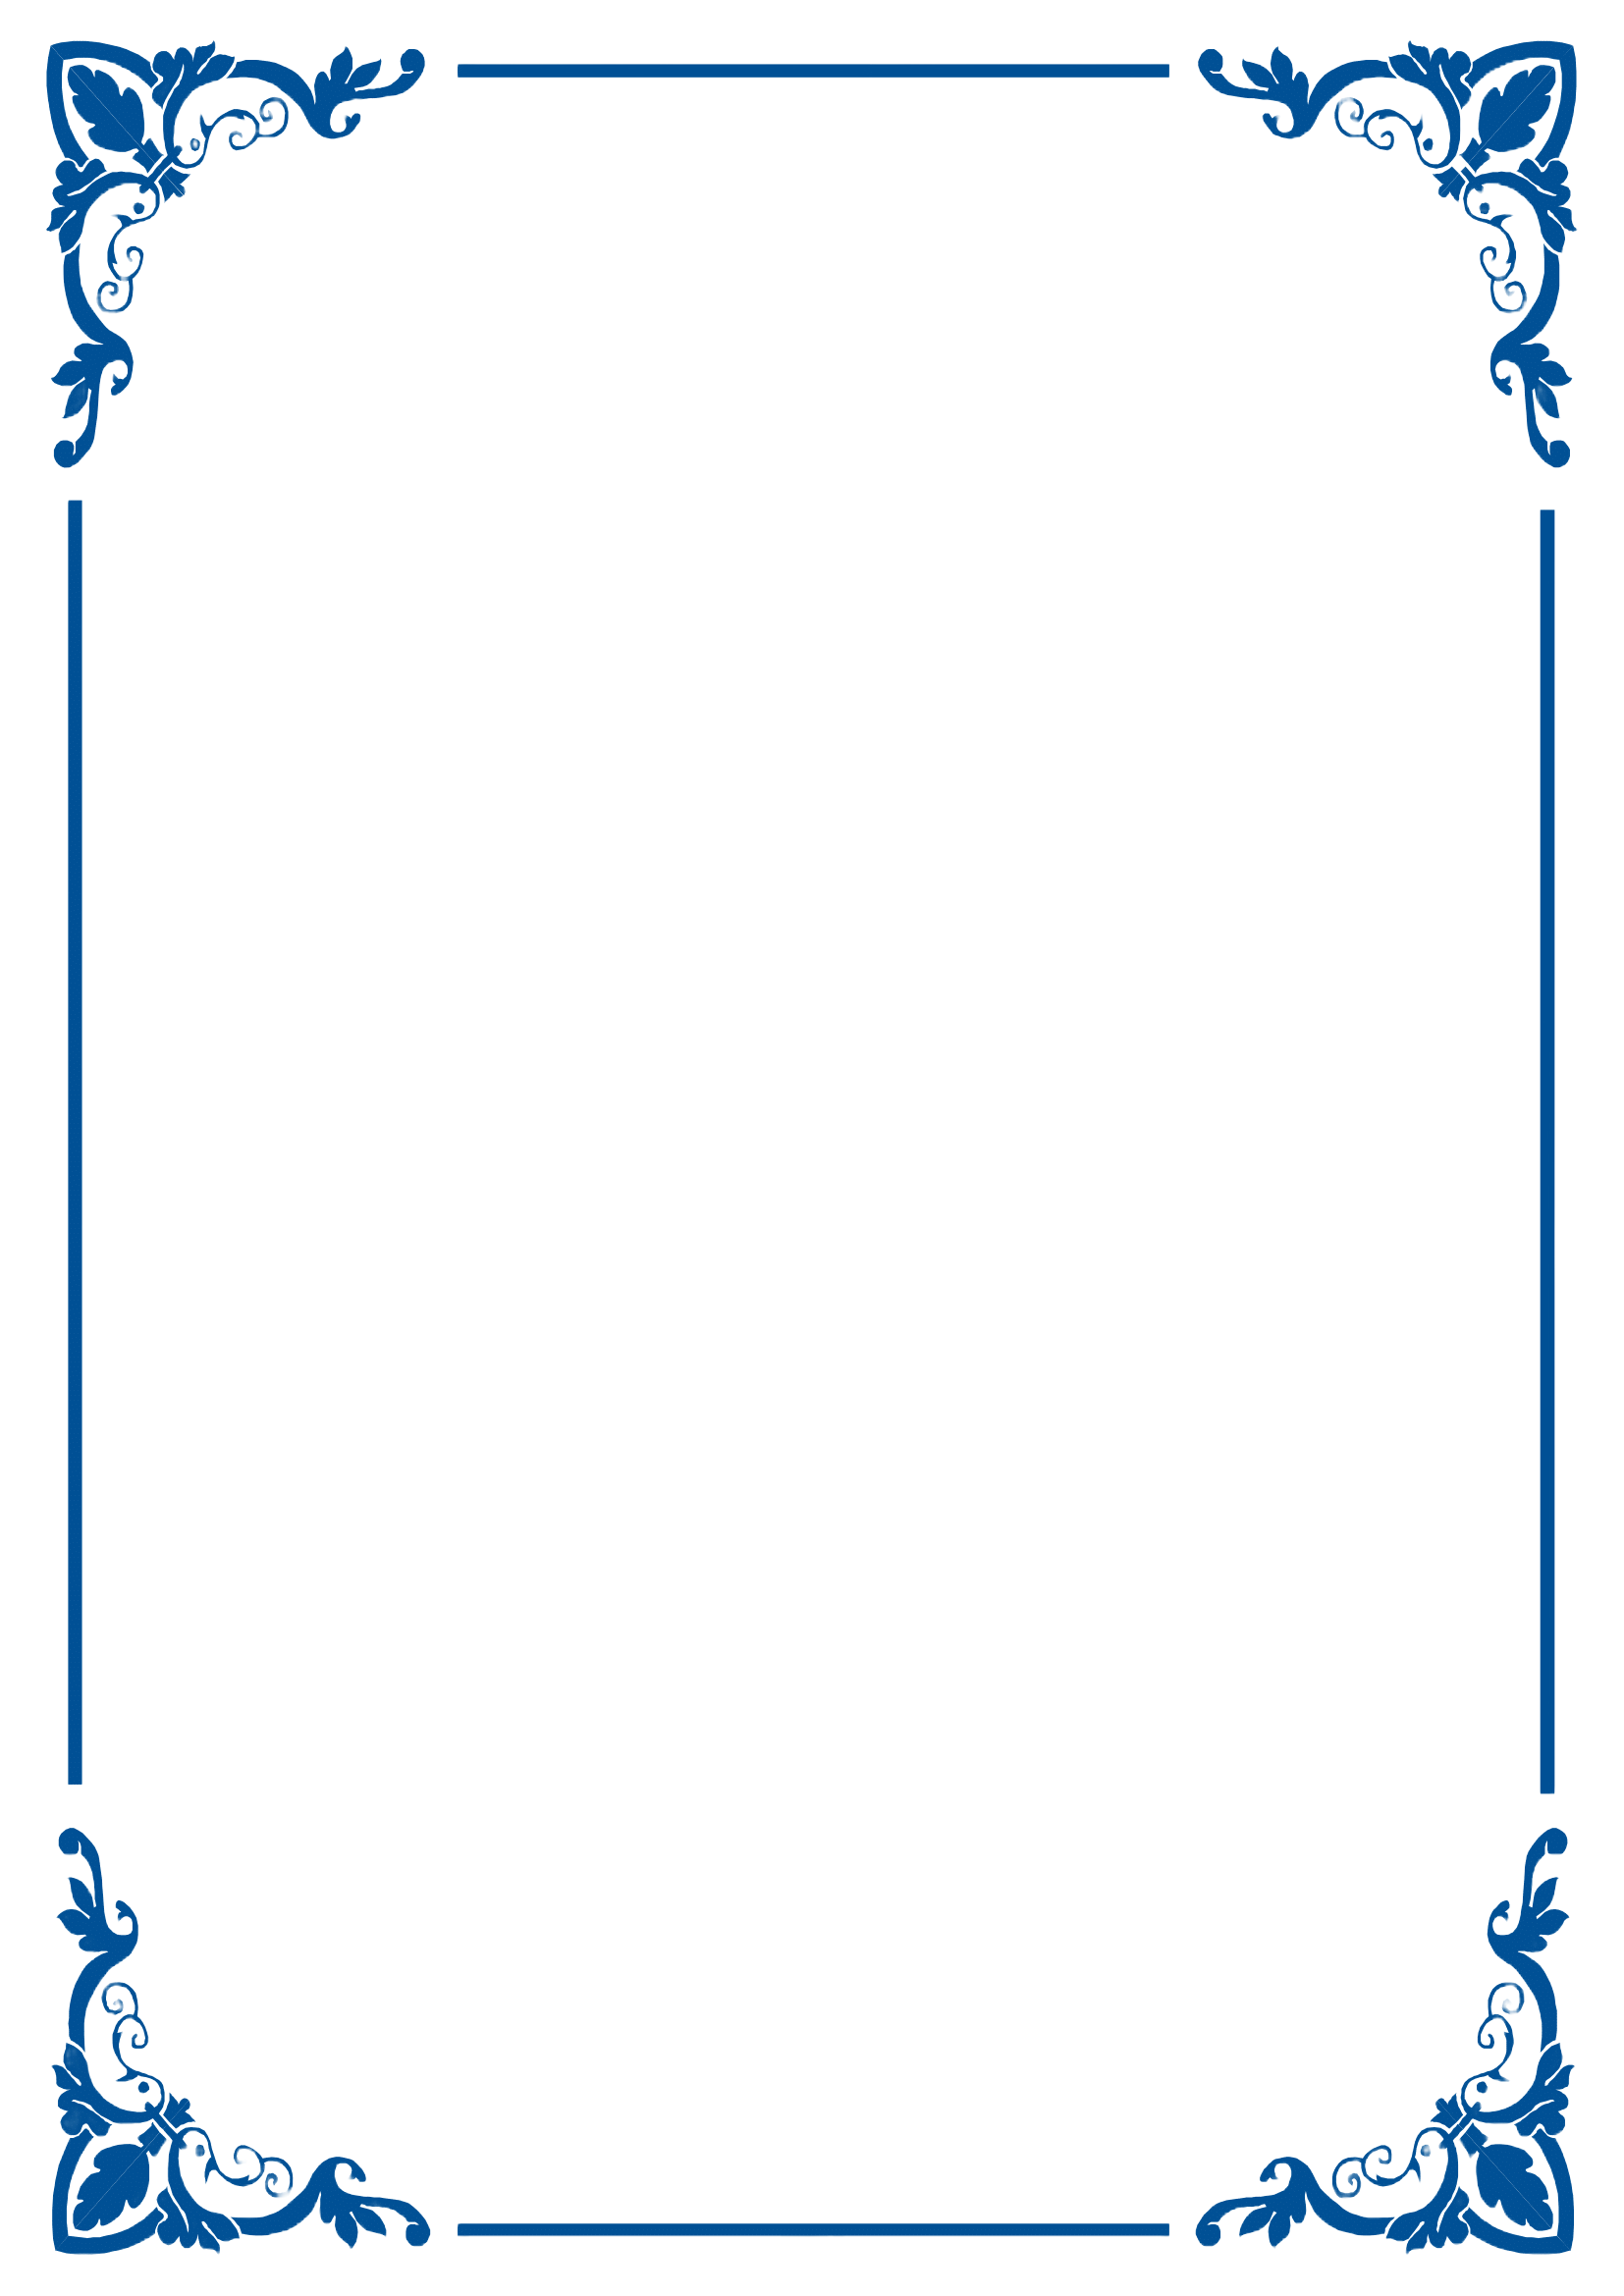
\includegraphics[width=19.4cm]{assets/khung_bia.png}};
	\end{tikzpicture}
}
\thispagestyle{empty}
\begin{adjustbox}{max totalsize={\textwidth}{\textheight},center}
\begin{minipage}{16.4cm}
\centering
\textbf{\large ĐẠI HỌC QUỐC GIA THÀNH PHỐ HỒ CHÍ MINH\\
	TRƯỜNG ĐẠI HỌC BÁCH KHOA\\
	KHOA KHOA HỌC ỨNG DỤNG}\\[2pt]
\rule{0.55\textwidth}{0.6pt}

\vspace{0.4cm}

\includegraphics[height=3.3cm]{assets/01_logobachkhoasang}

\vspace{0.4cm}
\textbf{\Large MÔ HÌNH THỐNG KÊ (AS3179)}

\vspace{0.3cm}
\noindent\rule{\textwidth}{0.8pt}\\[6pt]
{\large\textbf{BÀI TẬP LỚN}}\\[6pt]
{\Large\textbf{KIỂM CHỨNG THỰC NGHIỆM\\CÁC MÔ HÌNH ARMA VÀ ARIMA\\TRÊN DỮ LIỆU CHUỖI THỜI GIAN}}\\[6pt]
\noindent\rule{\textwidth}{0.8pt}

\vspace{0.5cm}
\large
\begin{tabular}{@{}r@{\hspace{0.8em}}l@{}}
	\textbf{Học kỳ:} & 261 \\
	\textbf{Lớp:} & L01 \\
	\textbf{Nhóm:} & 7 \\
	\textbf{Cặp bài giảng:} & Bài 11 và Bài 12 \\
	\textbf{Giảng viên:} & TS. Nguyễn Tiến Dũng \\
\end{tabular}

\vspace{0.5cm}
\textbf{Danh sách sinh viên thực hiện}\\[4pt]
\normalsize
\renewcommand{\arraystretch}{1.25}
\begin{tabular}{|c|l|l|c|p{3.2cm}|}
	\hline
	\textbf{STT} & \textbf{Họ} & \textbf{Tên} & \textbf{MSSV} & \textbf{Ghi chú} \\
	\hline
	1 & Lý Anh & Quân & 2412896 & \\
	\hline
	2 & Vũ Trần Hoàng & Quân & 2412928 & \\
	\hline
	3 & Hồ Lê Ngọc & Quang & 2412819 & \\
	\hline
	4 & Phạm Nhật & Quang & 2412846 & \\
	\hline
	5 & Phạm Anh & Quốc & 2412939 & \\
	\hline
\end{tabular}

\vspace{0.6cm}
\large\textbf{\textit{Thành phố Hồ Chí Minh, tháng 11 năm 2026}}
\end{minipage}
\end{adjustbox}
\newpage

% ================= ĐẦU/CHÂN TRANG VÀ MỤC LỤC =================
\pagestyle{fancy}
\renewcommand{\footrulewidth}{1pt}
\fancyhead{}
\lhead{
\includegraphics[width=5.2cm]{assets/bklogo}}
\rhead{\textbf{\normalsize {\color{blue}Mô hình thống kê - HK261}\\ \footnotesize{Nhóm 7 - Lớp L01}}}
\fancyfoot{}
\rfoot{Trang \thepage}
\setcounter{page}{1}

% ================= LỜI CẢM ƠN, LỜI NÓI ĐẦU =================
% LỜI CẢM ƠN: đặt ngay sau trang bìa, trước Lời nói đầu và Mục lục.
\clearpage
\section*{LỜI CẢM ƠN}
\addcontentsline{toc}{section}{Lời cảm ơn}

Nhóm chúng em xin gửi lời cảm ơn chân thành đến TS. Nguyễn Tiến Dũng, giảng viên môn Mô hình thống kê. Hai bài giảng về chuỗi thời gian của thầy là nền tảng của báo cáo này, và yêu cầu kiểm chứng lý thuyết bằng dữ liệu thực của thầy đã giúp nhóm hiểu bản chất của từng kết quả thay vì chỉ áp dụng công thức.

Nhóm cũng xin cảm ơn Khoa Khoa học Ứng dụng và Trường Đại học Bách Khoa, Đại học Quốc gia Thành phố Hồ Chí Minh, đã tạo điều kiện để nhóm được học tập và thực hiện bài tập lớn này. Báo cáo sử dụng các bộ dữ liệu từ kho Rdatasets và các thư viện mã nguồn mở của Python, nên nhóm xin ghi nhận công sức của những người đã xây dựng và chia sẻ các công cụ ấy.

Cuối cùng, các thành viên trong nhóm xin cảm ơn nhau vì sự phối hợp và tinh thần trách nhiệm trong suốt quá trình thực hiện. Do thời gian và kinh nghiệm còn hạn chế, báo cáo khó tránh khỏi thiếu sót, và nhóm rất mong nhận được góp ý của thầy để hoàn thiện hơn.

\vspace{1cm}
\hfill\begin{minipage}{8cm}
\centering
\textit{Thành phố Hồ Chí Minh, tháng 11 năm 2026}\\[2pt]
\textbf{Nhóm 7}
\end{minipage}

% LỜI NÓI ĐẦU: đặt sau Lời cảm ơn, trước Mục lục; nêu lý do chọn đề tài và cách đọc báo cáo, không lặp lại Chương 1.
\clearpage
\section*{LỜI NÓI ĐẦU}
\addcontentsline{toc}{section}{Lời nói đầu}

Chuỗi thời gian xuất hiện ở hầu hết các lĩnh vực, từ mực nước hồ và lưu lượng sông đến giá chứng khoán và lượng hành khách hàng không. Các mô hình ARMA và ARIMA là công cụ cổ điển để mô tả và dự báo những chuỗi này, nhưng lý thuyết của chúng dựa trên các giả thiết mà dữ liệu thực không phải lúc nào cũng thỏa mãn. Vì vậy nhóm chọn cách học bằng thực nghiệm: lấy từng kết quả lý thuyết, chạy nó trên dữ liệu thực bằng Python, rồi đối chiếu xem lý thuyết nói gì và dữ liệu cho thấy gì.

Báo cáo này là kết quả của quá trình đó. Thay vì nhắc lại toàn bộ lý thuyết, báo cáo chỉ tóm tắt những gì cần cho việc kiểm chứng ở \chg{2}, rồi đi thẳng vào kiểm chứng ở \chg{4}, \chn{5} và \chn{6}. Mỗi kết quả đều có đủ phần phát biểu, cách làm, mã lệnh, số liệu, diễn giải và nhận xét, nên người đọc có thể theo dõi hoặc tự chạy lại. Nơi nào kết quả khớp lý thuyết, nhóm nói rõ; nơi nào lệch, nhóm cố gắng chỉ ra lý do.

Để đọc thuận tiện, các bộ dữ liệu được gọi bằng những ký hiệu ngắn như HU, LY hay DR, và mọi chữ viết tắt đều được giải thích trong Danh mục ký hiệu và chữ viết tắt ngay sau Mục lục. Người đã quen với lý thuyết có thể đọc thẳng các chương kiểm chứng, còn các nhận xét tổng hợp nằm ở \chg{7} và \chg{8}. Mã nguồn đầy đủ và cách chạy lại có trong \phuluc{B}.

Nhóm hy vọng báo cáo này vừa chính xác vừa dễ theo dõi, và mong nhận được những góp ý để hoàn thiện hơn.

\clearpage

{\hypersetup{linkcolor=black}\setstretch{0.84}\tableofcontents\thispagestyle{fancy}}
\newpage

% ================= NỘI DUNG =================
% DANH MỤC KÝ HIỆU VÀ CHỮ VIẾT TẮT: đặt sau Mục lục, trước Chương 1; mọi ký hiệu hoặc chữ viết tắt mới xuất hiện trong báo cáo được thêm vào bảng này.
\clearpage
\phantomsection
\section*{DANH MỤC KÝ HIỆU VÀ CHỮ VIẾT TẮT}
\addcontentsline{toc}{section}{Danh mục ký hiệu và chữ viết tắt}

\begin{center}
\small
\renewcommand{\arraystretch}{1.2}
\begin{tabular}{|p{2.6cm}|p{14.4cm}|}
\toprule
Ký hiệu & Ý nghĩa \\
\midrule
\multicolumn{2}{|l|}{\textit{Bộ dữ liệu}} \\
HU & Hồ Huron: mực nước hồ hằng năm \\
LY & Linh miêu: logarit số linh miêu bị bẫy hằng năm \\
DR & DAX dạng suất sinh lợi: suất sinh lợi log hằng ngày của chỉ số DAX \\
NI & Nile: lưu lượng hằng năm của sông Nile \\
AP & AirPassengers: logarit số hành khách hàng không hằng tháng \\
DP & DAX dạng log giá: logarit giá đóng cửa hằng ngày của chỉ số DAX \\
DAX, SMI & chỉ số chứng khoán của Đức, chỉ số chứng khoán của Thụy Sĩ \\
DL1--DL6 & nguồn dữ liệu đánh số trong mục Tài liệu tham khảo \\
\midrule
\multicolumn{2}{|l|}{\textit{Mô hình}} \\
AR & tự hồi quy (autoregressive) \\
MA & trung bình trượt (moving average) \\
ARMA & tự hồi quy trung bình trượt \\
ARIMA & ARMA cho chuỗi đã lấy sai phân (tích hợp) \\
SARIMA & ARIMA có thành phần mùa vụ \\
GARCH & mô hình phương sai có điều kiện thay đổi theo thời gian \\
$I(d)$ & chuỗi tích hợp bậc $d$, tức chuỗi dừng sau $d$ lần lấy sai phân \\
WN, iid & nhiễu trắng; độc lập và cùng phân phối \\
\midrule
\multicolumn{2}{|l|}{\textit{Phương pháp ước lượng và kiểm định}} \\
ACF, PACF & hàm tự tương quan, hàm tự tương quan riêng phần \\
YW, OLS, ML & ước lượng Yule--Walker, bình phương tối thiểu, cực đại hợp lý \\
LB, $Q_{LB}$ & kiểm định Ljung--Box và thống kê của nó \\
ADF, KPSS & kiểm định nghiệm đơn vị Dickey--Fuller mở rộng; kiểm định tính dừng Kwiatkowski--Phillips--Schmidt--Shin \\
DM & kiểm định Diebold--Mariano \\
AIC, BIC & tiêu chuẩn thông tin Akaike, tiêu chuẩn thông tin Bayes \\
SD, SE & độ lệch chuẩn; sai số chuẩn \\
\midrule
\multicolumn{2}{|l|}{\textit{Thước đo sai số}} \\
MAE, RMSE & sai số tuyệt đối trung bình; căn bậc hai của sai số bình phương trung bình \\
MAPE, MASE & sai số phần trăm tuyệt đối trung bình; sai số tuyệt đối trung bình đã chuẩn hóa \\
MCSE & sai số Monte Carlo của một kết quả mô phỏng \\
\midrule
\multicolumn{2}{|l|}{\textit{Quy ước trong báo cáo}} \\
CH1--CH3 & ba câu hỏi nghiên cứu nêu ở \muc{1.2} \\
P, M, K & xếp loại phù hợp, phù hợp một phần, không phù hợp \\
\bottomrule
\end{tabular}
\end{center}

% CHƯƠNG 1. GIỚI THIỆU
\clearpage
\section[Giới thiệu]{GIỚI THIỆU}

\subsection{Bối cảnh}
Chuỗi thời gian là một dãy quan sát ghi theo thứ tự thời gian. Khác với dữ liệu thông thường, các quan sát liền nhau thường không độc lập: mực nước năm nay phụ thuộc mực nước năm trước, giá hôm nay liên quan đến giá hôm qua. Sự phụ thuộc này vừa là điều cần mô tả, vừa khiến các phương pháp dành cho dữ liệu độc lập không dùng được nguyên vẹn.

ARMA và ARIMA là công cụ nền tảng để mô tả sự phụ thuộc ấy và để dự báo. Lý thuyết của chúng dựa trên những giả thiết gọn, như chuỗi dừng, nhiễu có tính chất cho trước và mô hình đúng bậc, trong khi dữ liệu thực hiếm khi thỏa mãn hoàn hảo vì có thể trôi, đổi mức, có mùa vụ hoặc có biến động thay đổi theo thời gian. Câu hỏi tự nhiên là lý thuyết còn đúng đến đâu trên dữ liệu thực, và khi lệch thì lệch vì lý do gì. Báo cáo này đi tìm lời đáp cho câu hỏi đó.

\subsection{Mục tiêu}
Mục tiêu chung là kiểm chứng bằng Python các kết quả lý thuyết về chuỗi dừng, ARMA, chuỗi không dừng, ARIMA và dự báo trên sáu bộ dữ liệu thực, kết hợp mô phỏng khi cần, rồi đánh giá mức độ phù hợp giữa lý thuyết và thực nghiệm. Cụ thể, báo cáo trả lời ba câu hỏi sau:
\begin{enumerate}[label=\textbf{CH\arabic*.}]
	\item Các kết quả lý thuyết về cấu trúc phụ thuộc và mô hình ARMA có được thỏa mãn trên dữ liệu thực hay không?
	\item Các kết quả lý thuyết về chuỗi không dừng, mô hình ARIMA và dự báo có được thỏa mãn trên dữ liệu thực hay không?
	\item Mức độ phù hợp phụ thuộc thế nào vào đặc điểm của từng bộ dữ liệu, và giả thiết nào bị vi phạm?
\end{enumerate}

\subsection{Phạm vi}
Nhóm chọn cặp Bài giảng 11 và 12 của học phần AS3179 \tlk{14,15}. Bài 11, \textit{Chuỗi thời gian I: Phụ thuộc và mô hình ARMA}, được kiểm chứng ở \chg{4} trên ba bộ dữ liệu HU, LY và DR. Bài 12, \textit{Chuỗi thời gian II: ARIMA và dự báo}, được kiểm chứng ở \chg{5} và \chn{6} trên ba bộ dữ liệu NI, AP và DP. Sáu bộ dữ liệu này đều lấy từ R và được mô tả cùng nguồn gốc ở Bảng~\ref{tab:dulieu}. Chúng được ký hiệu theo Danh mục ký hiệu và chữ viết tắt ở đầu báo cáo, và các phần sau chỉ gọi bằng các ký hiệu ấy. Hai ký hiệu DR và DP cùng chỉ số DAX nhưng ở hai dạng khác nhau, vì suất sinh lợi là dạng dừng còn log giá là dạng không dừng của cùng một chuỗi.
Về phương pháp, báo cáo dùng mô hình ARMA, ARIMA và ARIMA mùa vụ cùng các công cụ đi kèm là tự tương quan, kiểm định Ljung--Box, kiểm định nghiệm đơn vị và kiểm định Diebold--Mariano. Các mô hình như GARCH, Prophet hay học máy nằm ngoài phạm vi, dù có những chuỗi, điển hình là DR, mang đặc điểm mà các mô hình đó xử lý tốt hơn.

Nội dung kiểm chứng gồm 28 kết quả lý thuyết, được liệt kê cùng ký hiệu bộ dữ liệu áp dụng trong Bảng~\ref{tab:danhmuc}. Trong số đó, 18 kết quả được kiểm chứng bằng dữ liệu thực, 10 bằng cả dữ liệu thực lẫn mô phỏng.

{\footnotesize
\begin{longtable}{|p{2.2cm}|p{6.6cm}|p{5.2cm}|p{2.2cm}|}
\caption{Danh mục các nội dung kiểm chứng}\label{tab:danhmuc}\\
\toprule
Địa chỉ & Nội dung & Ký hiệu bộ dữ liệu áp dụng & Hình thức \\
\midrule
\endfirsthead
\toprule
Địa chỉ & Nội dung & Ký hiệu bộ dữ liệu áp dụng & Hình thức \\
\midrule
\endhead
\bottomrule
\endlastfoot
\ndlk{4.1(a)} & Tính dừng và nhiễu trắng & HU, LY, DR & Dữ liệu thực \\
\ndlk{4.1(b)} & Tính chất của tự hiệp phương sai & HU, LY, DR & Dữ liệu thực \\
\ndlk{4.1(c)} & Trung bình mẫu của chuỗi phụ thuộc & HU, LY, DR & Cả hai \\
\ndlk{4.1(d)} & Quá trình tuyến tính & HU, LY, DR & Dữ liệu thực \\
\ndlk{4.2(a)} & Mô hình AR(1) & HU, LY, DR & Cả hai \\
\ndlk{4.2(b)} & Mô hình AR(p) và hệ Yule–Walker & LY, HU, DR & Dữ liệu thực \\
\ndlk{4.2(c)} & Mô hình AR(2) & HU, LY, DR & Dữ liệu thực \\
\ndlk{4.2(d)} & Mô hình MA(q) & HU, LY, DR & Cả hai \\
\ndlk{4.2(e)} & Mô hình ARMA(p, q) & HU, LY, DR & Cả hai \\
\ndlk{4.3(a)} & Tự tương quan và kiểm định Ljung–Box & HU, LY, DR & Cả hai \\
\ndlk{4.3(b)} & Tự tương quan riêng phần & HU, LY, DR & Dữ liệu thực \\
\ndlk{4.3(c)} & Ước lượng tham số & LY, HU, DR & Cả hai \\
\ndlk{4.3(d)} & Lựa chọn bậc & LY, HU, DR & Dữ liệu thực \\
\ndlk{4.3(e)} & Chẩn đoán phần dư & HU, LY, DR & Dữ liệu thực \\
\ndlk{5.1(a)} & Xu thế tất định và ngẫu nhiên & NI, AP, DP & Dữ liệu thực \\
\ndlk{5.1(b)} & Bước ngẫu nhiên & NI, AP, DP & Cả hai \\
\ndlk{5.2(a)} & Mô hình ARIMA và độ trôi & NI, AP, DP & Dữ liệu thực \\
\ndlk{5.2(b)} & Mô hình ARIMA mùa vụ & NI, AP, DP & Dữ liệu thực \\
\ndlk{5.3(a)} & Sai phân và sai phân quá mức & NI, AP, DP & Cả hai \\
\ndlk{5.3(b)} & Kiểm định nghiệm đơn vị & NI, AP, DP & Cả hai \\
\ndlk{6.1(a)} & Ảnh hưởng vĩnh viễn của cú sốc & NI, AP, DP & Dữ liệu thực \\
\ndlk{6.1(b)} & Làm trơn mũ và mô hình mức cục bộ & NI, AP, DP & Dữ liệu thực \\
\ndlk{6.2(a)} & Dự báo tối ưu và khoảng dự báo & NI, AP, DP & Cả hai \\
\ndlk{6.2(b)} & Dự báo trên thang logarit & NI, AP, DP & Dữ liệu thực \\
\ndlk{6.3(a)} & Mốc chuẩn và thước đo sai số & NI, AP, DP & Dữ liệu thực \\
\ndlk{6.3(b)} & Gốc cuốn chiếu & NI, AP, DP & Dữ liệu thực \\
\ndlk{6.3(c)} & Hàm mất mát và kiểm định Diebold–Mariano & NI, AP, DP & Dữ liệu thực \\
\ndlk{6.3(d)} & Quy trình báo cáo dự báo & NI, AP, DP & Dữ liệu thực \\
\end{longtable}}

\subsection{Bố cục}
Báo cáo gồm tám chương. \chg{2} trình bày cơ sở lý thuyết theo ba mục là chuỗi dừng và ARMA, chuỗi không dừng và ARIMA, dự báo và đánh giá dự báo. \chg{3} giới thiệu dữ liệu và phương pháp. Ba mục của \chg{2} lần lượt được kiểm chứng ở các \chg{4}, \chn{5} và \chn{6}, sau đó \chg{7} thảo luận chung và \chg{8} kết luận.

Mỗi kết quả ở \chg{2} mang một địa chỉ dạng \texttt{2.m.n(z)} và được kiểm chứng tại mục có địa chỉ \texttt{(m+3).n(z)}; chẳng hạn kết quả \texttt{2.1.2(c)} được kiểm chứng tại \texttt{4.2(c)}. Mỗi nội dung kiểm chứng gồm sáu phần: kết quả cần kiểm chứng, cách triển khai, mã Python, kết quả tính toán, phân tích và diễn giải, và nhận xét. Phần nhận xét xếp loại kết quả thành \emph{phù hợp}, \emph{phù hợp một phần} hoặc \emph{không phù hợp} theo thang trong Bảng~\ref{tab:thangdo}.

% CHƯƠNG 2. CƠ SỞ LÝ THUYẾT: chỉ phát biểu kết quả (không chứng minh). Mọi lý thuyết của báo cáo nằm ở chương này.
% Ba mục 2.1, 2.2, 2.3 tương ứng ba chương kiểm chứng 4, 5, 6; mục con 2.m.n(z) được kiểm chứng tại (m+3).n(z).
\clearpage
\section[Cơ sở lý thuyết]{CƠ SỞ LÝ THUYẾT}

Chương này tổng hợp kiến thức lý thuyết mà các chương sau dùng đến, theo mạch từ đơn giản đến phức tạp. \Muc{2.1} nói về chuỗi dừng và mô hình ARMA, \muc{2.2} về chuỗi không dừng và mô hình ARIMA, còn \muc{2.3} về dự báo và đánh giá dự báo. Các kết quả được phát biểu gọn cùng điều kiện áp dụng và không chứng minh, vì phần chứng minh có trong \tlk{2,3}. Mỗi kết quả mang một địa chỉ \texttt{2.m.n(z)} và được kiểm chứng ở \chg{4}, \chn{5} hoặc \chn{6} tùy mục chứa nó; địa chỉ trong chương kiểm chứng chỉ cần cộng $3$ vào số mục, chẳng hạn \texttt{2.1.2(b)} được kiểm chứng tại \texttt{4.2(b)}. Các ký hiệu toán học chính được tóm tắt trong Bảng~\ref{tab:kyhieu}.

\begin{table}[H]
\centering\small
\caption{Các ký hiệu chính}\label{tab:kyhieu}
\renewcommand{\arraystretch}{1.25}
\begin{tabular}{|p{3.4cm}|p{12.6cm}|}
\toprule
Ký hiệu & Ý nghĩa \\
\midrule
$\{Y_t\}$, $y_1,\dots,y_n$ & chuỗi thời gian, coi như quá trình ngẫu nhiên, và dữ liệu quan sát \\
$\varepsilon_t\sim WN(0,\sigma^2)$ & nhiễu trắng có trung bình $0$, phương sai $\sigma^2$ \\
$B$, $\nabla=1-B$, $\nabla_s=1-B^s$ & toán tử lùi $BY_t=Y_{t-1}$, toán tử sai phân và sai phân mùa vụ chu kỳ $s$ \\
$\gamma(h)$, $\rho(h)$, $\alpha(h)$ & tự hiệp phương sai, tự tương quan và tự tương quan riêng phần tại độ trễ $h$; dạng mẫu: $\hat\gamma(h)$, $\hat\rho(h)$, $\hat\alpha(h)$ \\
$\phi(z)$, $\theta(z)$ & đa thức AR $1-\phi_1z-\dots-\phi_pz^p$ và đa thức MA $1+\theta_1z+\dots+\theta_qz^q$ \\
$\psi_j$, $\Psi_j$ & hệ số của $\theta(z)/\phi(z)$ và của $\theta(z)/\{\phi(z)(1-z)^d\}$ \\
$Q_{LB}(H)$ & thống kê Ljung--Box với $H$ độ trễ \\
$\hat Y_{n+h|n}$, $e_n(h)$ & dự báo $h$ bước tại thời điểm $n$ và sai số dự báo tương ứng \\
\bottomrule
\end{tabular}
\end{table}

% ======================= Chuỗi dừng và mô hình ARMA =======================
\subsection{Chuỗi dừng và mô hình ARMA}

Mọi mô hình trong báo cáo bắt đầu từ một câu hỏi: cấu trúc phụ thuộc của chuỗi có ổn định theo thời gian hay không? Mục này trình bày khái niệm chuỗi dừng, họ mô hình ARMA, rồi cách nhận dạng, ước lượng và kiểm tra mô hình. Nội dung được kiểm chứng ở \chg{4}.

\subsubsection{Chuỗi dừng}

\noidung{Tính dừng và nhiễu trắng}
Dữ liệu ta có chỉ là một dãy số $y_1,\dots,y_n$ quan sát một lần, coi như một mẫu của dãy biến ngẫu nhiên $\{Y_t,\ t\in\mathbb Z\}$. Để từ một mẫu duy nhất rút ra điều gì đó, ta cần giả thiết đặc trưng của chuỗi không đổi theo thời gian: đó là tính dừng. Khi $\E Y_t^2<\infty$, hai đặc trưng cần quan tâm là hàm trung bình $\mu_t=\E Y_t$ và hàm tự hiệp phương sai $\gamma(s,t)=\Cov(Y_s,Y_t)$.
\begin{kq}
\begin{enumerate}[label=(\roman*),leftmargin=*,itemsep=1pt]
\item \emph{Dừng nghiêm ngặt:} $(Y_{t_1+h},\dots,Y_{t_k+h})$ có cùng phân phối đồng thời với $(Y_{t_1},\dots,Y_{t_k})$ với mọi $k$, mọi $t_1,\dots,t_k$ và mọi độ dịch $h$.
\item \emph{Dừng yếu:} $\E Y_t^2<\infty$, $\mu_t\equiv\mu$ không đổi và $\gamma(t+h,t)=\gamma(h)$ chỉ phụ thuộc độ trễ $h$. Hàm tự tương quan là $\rho(h)=\gamma(h)/\gamma(0)$.
\item \emph{Nhiễu trắng} $\varepsilon_t\sim WN(0,\sigma^2)$: dừng yếu, trung bình $0$, $\gamma(0)=\sigma^2$ và $\gamma(h)=0$ với $h\neq0$. Nếu các $\varepsilon_t$ còn độc lập và cùng phân phối thì gọi là \emph{nhiễu iid}.
\end{enumerate}
\end{kq}
Nói đơn giản, chuỗi dừng yếu có mức trung bình cố định và độ phụ thuộc giữa hai thời điểm chỉ phụ thuộc khoảng cách giữa chúng. Dừng nghiêm ngặt kéo theo dừng yếu khi $\E Y_t^2<\infty$, và với quá trình Gauss hai khái niệm trùng nhau; từ đây ``dừng'' được hiểu là dừng yếu. Cũng cần phân biệt nhiễu trắng với nhiễu iid, vốn là điều kiện mạnh hơn: suất sinh lợi tài chính thường không tự tương quan nhưng bình phương của chúng thì có, vì biến động lớn tụ thành từng cụm, và điều này giúp ta đọc đúng phần dư ở \muc{2.1.3}.

\kiemchung{4.1(a)}

\noidung{Tính chất của tự hiệp phương sai}
Không phải hàm nào cũng có thể là tự hiệp phương sai của một chuỗi dừng; nó phải thỏa mãn một số tính chất.
\begin{kq}
Giả sử $\gamma$ là hàm tự hiệp phương sai của một chuỗi dừng yếu. Khi đó:
\begin{enumerate}[label=(\roman*),leftmargin=*,itemsep=1pt]
\item $\gamma(0)\ge0$ và $|\gamma(h)|\le\gamma(0)$, nên $|\rho(h)|\le1$;
\item $\gamma(-h)=\gamma(h)$, tức $\gamma$ là hàm chẵn;
\item $\gamma$ xác định không âm: $\sum_{i,j=1}^{k}a_ia_j\gamma(t_i-t_j)\ge0$ với mọi $k$, mọi số thực $a_i$ và mọi thời điểm $t_i$. Tương đương, ma trận Toeplitz $\Gamma_n=[\gamma(i-j)]_{i,j=1}^{n}$, chính là ma trận hiệp phương sai của $(Y_1,\dots,Y_n)$, xác định không âm.
\end{enumerate}
\end{kq}
Từ dữ liệu, tự hiệp phương sai mẫu và tự tương quan mẫu tại độ trễ $0\le h<n$ được tính bởi
\[
\hat\gamma(h)=\frac1n\sum_{t=1}^{n-h}(y_{t+h}-\bar y)(y_t-\bar y),\qquad \hat\rho(h)=\frac{\hat\gamma(h)}{\hat\gamma(0)},\qquad \hat\gamma(-h)=\hat\gamma(h).
\]
Ta chia cho $n$ chứ không phải $n-h$ vì cách này bảo đảm $\hat\Gamma_n$ xác định không âm, nhờ đó mô hình AR khớp bằng Yule--Walker luôn nhân quả, như sẽ thấy ở \muc{2.1.3}. Cái giá là $\hat\gamma(h)$ hơi chệch ở độ trễ lớn, nên chỉ đọc $\hat\rho(h)$ khi $h$ nhỏ so với $n$, thường là $h\le n/4$. Khi chuỗi có xu thế hoặc dịch mức, $\hat\rho(h)$ giảm rất chậm, phản ánh tính không dừng chứ không phải ``trí nhớ'' thật sự.
\kiemchung{4.1(b)}

\noidung{Trung bình mẫu của chuỗi phụ thuộc}
Với dữ liệu độc lập, trung bình mẫu $\bar Y=\frac1n\sum_{t=1}^nY_t$ có phương sai $\gamma(0)/n$. Khi các quan sát phụ thuộc nhau thì công thức này không còn đúng nữa.
\begin{kq}
Cho $\{Y_t\}$ dừng yếu với trung bình $\mu$ và tự hiệp phương sai $\gamma$. Khi đó:
\begin{enumerate}[label=(\roman*),leftmargin=*,itemsep=1pt]
\item $\E\bar Y=\mu$ và $\displaystyle\Var\bar Y=\frac1n\sum_{|h|<n}\Bigl(1-\frac{|h|}{n}\Bigr)\gamma(h)$.
\item Nếu $\sum_h|\gamma(h)|<\infty$ thì $n\Var\bar Y\to\sum_{h=-\infty}^{\infty}\gamma(h)=\gamma(0)\,\tau$, với $\tau=1+2\sum_{h\ge1}\rho(h)$. Đại lượng $n_{\mathrm{eff}}=n/\tau$ gọi là \emph{cỡ mẫu hiệu dụng}. Với AR(1), $\tau=(1+\phi)/(1-\phi)$.
\item Nếu thêm $Y_t=\mu+\sum_j\psi_j\varepsilon_{t-j}$ với $\varepsilon_t$ iid và $\sum_j|\psi_j|<\infty$ thì $\sqrt n(\bar Y-\mu)\xrightarrow{d}N\bigl(0,\gamma(0)\tau\bigr)$.
\end{enumerate}
\end{kq}
Khi các quan sát tự tương quan dương, tức $\tau>1$, $n$ quan sát chỉ mang lượng thông tin của khoảng $n/\tau$ quan sát độc lập. Vì vậy sai số chuẩn $s/\sqrt n$ quen thuộc quá lạc quan: khoảng $\bar y\pm1.96\,s/\sqrt n$ phủ ít hơn $95\%$, còn khoảng đúng là $\bar y\pm1.96\,s\sqrt{\tau/n}$, với $\tau$ ước lượng từ mô hình đã khớp hoặc từ ACF mẫu. Nguyên lý này cũng áp dụng cho sai số chuẩn của hệ số hồi quy khi sai số tự tương quan, chẳng hạn hệ số dốc của xu thế.
\kiemchung{4.1(c)}

\noidung{Quá trình tuyến tính}
Ta dùng toán tử lùi $B$, xác định bởi $BY_t=Y_{t-1}$ và do đó $B^jY_t=Y_{t-j}$. Với đa thức AR $\phi(z)=1-\phi_1z-\dots-\phi_pz^p$, viết gọn $\phi(B)Y_t=Y_t-\phi_1Y_{t-1}-\dots-\phi_pY_{t-p}$.
\begin{kq}
\begin{enumerate}[label=(\roman*),leftmargin=*,itemsep=1pt]
\item \emph{Quá trình tuyến tính} là chuỗi $Y_t=\mu+\sum_{j=-\infty}^{\infty}\psi_j\varepsilon_{t-j}$ với $\varepsilon_t\sim WN(0,\sigma^2)$ và $\sum_j|\psi_j|<\infty$. Nó \emph{nhân quả} nếu $\psi_j=0$ với mọi $j<0$, nghĩa là $Y_t$ chỉ phụ thuộc nhiễu ở hiện tại và quá khứ.
\item Quá trình tuyến tính là dừng yếu, có trung bình $\mu$ và $\gamma(h)=\sigma^2\sum_j\psi_j\psi_{j+h}$.
\end{enumerate}
\end{kq}
Mọi mô hình ARMA ở \muc{2.1.2} đều quy về quá trình tuyến tính nhân quả, nên ý (ii) cho cách tính tự hiệp phương sai từ các $\psi_j$.
\kiemchung{4.1(d)}

\subsubsection{Mô hình ARMA}

Giá trị hiện tại của chuỗi phụ thuộc vào chính quá khứ của nó, qua phần tự hồi quy AR, và vào các cú sốc ngẫu nhiên gần đây, qua phần trung bình trượt MA. Mô hình tự hồi quy bậc $p$, AR$(p)$, là $\phi(B)(Y_t-\mu)=\varepsilon_t$, hay $Y_t=c+\phi_1Y_{t-1}+\dots+\phi_pY_{t-p}+\varepsilon_t$ với $c=\mu(1-\phi_1-\dots-\phi_p)$. Phần này xét AR(1), AR$(p)$, AR(2), rồi MA$(q)$ và ARMA$(p,q)$.

\noidung{Mô hình AR(1)}
Đây là mô hình đơn giản nhất nhưng đã có đủ các đặc điểm cốt lõi của họ AR: $Y_t-\mu=\phi(Y_{t-1}-\mu)+\varepsilon_t$ với $\varepsilon_t\sim WN(0,\sigma^2)$.
\begin{kq}
\begin{enumerate}[label=(\roman*),leftmargin=*,itemsep=1pt]
\item Nếu $|\phi|<1$, nghiệm dừng duy nhất là quá trình tuyến tính nhân quả $Y_t=\mu+\sum_{j\ge0}\phi^j\varepsilon_{t-j}$.
\item Khi đó $\gamma(h)=\sigma^2\phi^{|h|}/(1-\phi^2)$ và $\rho(h)=\phi^{|h|}$: suy giảm theo hàm mũ, và đổi dấu xen kẽ nếu $\phi<0$.
\item Nếu $|\phi|=1$ thì không có nghiệm dừng với phương sai hữu hạn; nếu $|\phi|>1$ thì nghiệm dừng duy nhất $Y_t=\mu-\sum_{j\ge1}\phi^{-j}\varepsilon_{t+j}$ phụ thuộc vào tương lai. Vì vậy AR(1) dừng và nhân quả đòi hỏi $|\phi|<1$.
\item Dự báo tuyến tính tốt nhất của $Y_{n+h}$ từ $Y_n,Y_{n-1},\dots$ là $\mu+\phi^h(Y_n-\mu)$, với sai số bình phương trung bình $\sigma^2(1-\phi^{2h})/(1-\phi^2)\to\gamma(0)$ khi $h\to\infty$.
\end{enumerate}
\end{kq}
Có thể hình dung $\phi$ là độ ``dai dẳng'': mỗi kỳ, ảnh hưởng của một cú sốc còn lại $\phi$ lần, nên dự báo quay về $\mu$ nhanh nếu $|\phi|$ nhỏ và chậm nếu $|\phi|$ gần $1$. Trường hợp $|\phi|=1$ ở (iii), nơi cú sốc không bao giờ tắt, là điểm khởi đầu của \muc{2.2}.
\kiemchung{4.2(a)}

\noidung{Mô hình AR(p) và hệ Yule--Walker}
\begin{kq}
Cho $\phi(B)(Y_t-\mu)=\varepsilon_t$ với $\phi(z)=1-\phi_1z-\dots-\phi_pz^p$.
\begin{enumerate}[label=(\roman*),leftmargin=*,itemsep=1pt]
\item \emph{Tính nhân quả:} tồn tại nghiệm dừng nhân quả duy nhất khi và chỉ khi mọi nghiệm của $\phi(z)=0$ nằm ngoài vòng tròn đơn vị, $|z|>1$. Khi đó $Y_t=\mu+\sum_{j\ge0}\psi_j\varepsilon_{t-j}$ với $\sum_j\psi_jz^j=1/\phi(z)$ trên $|z|\le1$.
\item \emph{Phương trình Yule--Walker:} với AR$(p)$ nhân quả,
\[
\gamma(h)=\phi_1\gamma(h-1)+\dots+\phi_p\gamma(h-p)\ (h\ge1),\qquad \sigma^2=\gamma(0)-\phi_1\gamma(1)-\dots-\phi_p\gamma(p),
\]
hay ở dạng ma trận $\Gamma_p\boldsymbol\phi=\boldsymbol\gamma_p$, với $\Gamma_p=[\gamma(i-j)]_{i,j=1}^{p}$ và $\boldsymbol\gamma_p=(\gamma(1),\dots,\gamma(p))^\top$.
\item $\rho(h)$ thỏa cùng phương trình sai phân: nếu các nghiệm $z_1,\dots,z_p$ phân biệt thì $\rho(h)=\sum_ic_iz_i^{-|h|}$, là tổ hợp của các hàm mũ tắt dần ứng với nghiệm thực và các dao động sin tắt dần ứng với cặp nghiệm phức.
\end{enumerate}
\end{kq}
Điều kiện nghiệm ở (i) được kiểm tra mỗi khi khớp một mô hình AR, còn phương trình Yule--Walker ở (ii) cho phép tính $\rho(h)$ từ các hệ số hoặc ngược lại ước lượng hệ số từ $\hat\rho(h)$, như ở \muc{2.1.3}. Nghiệm nằm \emph{trên} vòng tròn đơn vị, $z=1$, là trường hợp đặc biệt dẫn sang \muc{2.2}.
\kiemchung{4.2(b)}

\noidung{Mô hình AR(2)}
Với $Y_t-\mu=\phi_1(Y_{t-1}-\mu)+\phi_2(Y_{t-2}-\mu)+\varepsilon_t$, điều kiện nhân quả và dạng của tự tương quan có thể đọc trực tiếp từ cặp $(\phi_1,\phi_2)$.
\begin{kq}
\begin{enumerate}[label=(\roman*),leftmargin=*,itemsep=1pt]
\item Mô hình nhân quả khi và chỉ khi $\phi_1+\phi_2<1$, $\ \phi_2-\phi_1<1$ và $|\phi_2|<1$, tức điểm $(\phi_1,\phi_2)$ nằm trong một hình tam giác.
\item $\rho(1)=\phi_1/(1-\phi_2)$ và $\rho(h)=\phi_1\rho(h-1)+\phi_2\rho(h-2)$.
\item Các nghiệm là phức khi và chỉ khi $\phi_1^2+4\phi_2<0$; khi đó $\rho(h)=a\,r^h\cos(\omega h+b)$ với $r=\sqrt{-\phi_2}$, $\cos\omega=\phi_1/(2r)$, còn $a,b$ được xác định bởi $\rho(0),\rho(1)$. Đó là một dao động tắt dần có chu kỳ $2\pi/\omega$.
\end{enumerate}
\end{kq}
AR(2) đáng chú ý vì mô tả được chuỗi có chu kỳ: số linh miêu bị bẫy hằng năm tăng giảm theo chu kỳ gần 10 năm, và AR(2) với nghiệm phức bắt được kiểu dao động này.
\kiemchung{4.2(c)}

\noidung{Mô hình MA(q)}
Mô hình trung bình trượt bậc $q$ là $Y_t=\mu+\theta(B)\varepsilon_t=\mu+\varepsilon_t+\theta_1\varepsilon_{t-1}+\dots+\theta_q\varepsilon_{t-q}$ với $\theta(z)=1+\theta_1z+\dots+\theta_qz^q$.
\begin{kq}
\begin{enumerate}[label=(\roman*),leftmargin=*,itemsep=1pt]
\item MA$(q)$ dừng với mọi $\theta_j$. Với $\theta_0=1$: $\gamma(h)=\sigma^2\sum_{j=0}^{q-|h|}\theta_j\theta_{j+|h|}$ khi $|h|\le q$ và $\gamma(h)=0$ khi $|h|>q$; tức ACF bị cắt cụt sau độ trễ $q$.
\item MA(1), $Y_t=\mu+\varepsilon_t+\theta\varepsilon_{t-1}$: $\rho(1)=\theta/(1+\theta^2)$, nên $|\rho(1)|\le\tfrac12$, dấu bằng xảy ra khi và chỉ khi $\theta=\pm1$.
\item Hai mô hình MA(1) với $(\theta,\sigma^2)$ và $(1/\theta,\theta^2\sigma^2)$ có cùng hàm tự hiệp phương sai. Mô hình có $|\theta|<1$ là \emph{khả nghịch}: $\varepsilon_t=\sum_{j\ge0}(-\theta)^j(Y_{t-j}-\mu)$.
\end{enumerate}
\end{kq}
Ý (iii) cho thấy hai mô hình khác nhau có thể có cùng ACF nên không phân biệt được qua ACF. Ta khắc phục bằng cách luôn chọn mô hình khả nghịch, tức mô hình có nhiễu $\varepsilon_t$ khôi phục được từ các quan sát hiện tại và quá khứ, và kiểm tra điều này sau khi ước lượng.
\kiemchung{4.2(d)}

\noidung{Mô hình ARMA(p, q)}
ARMA$(p,q)$ ghép hai phần trên lại: $\phi(B)(Y_t-\mu)=\theta(B)\varepsilon_t$, trong đó $\phi$ và $\theta$ không có nghiệm chung.
\begin{kq}
\begin{enumerate}[label=(\roman*),leftmargin=*,itemsep=1pt]
\item \emph{Nhân quả:} có nghiệm dừng nhân quả duy nhất khi và chỉ khi $\phi(z)\ne0$ với $|z|\le1$. Khi đó $Y_t=\mu+\sum_{j\ge0}\psi_j\varepsilon_{t-j}$ với $\sum_j\psi_jz^j=\theta(z)/\phi(z)$ và $\gamma(h)=\sigma^2\sum_{j\ge0}\psi_j\psi_{j+|h|}$.
\item \emph{Khả nghịch:} khi và chỉ khi $\theta(z)\ne0$ với $|z|\le1$; khi đó $\sum_j\pi_jz^j=\phi(z)/\theta(z)$.
\item \emph{ARMA(1,1)} ($|\phi|<1$, $\phi+\theta\ne0$): $\psi_0=1$, $\psi_j=(\phi+\theta)\phi^{j-1}$ với $j\ge1$;
\[
\gamma(0)=\sigma^2\,\frac{1+2\phi\theta+\theta^2}{1-\phi^2},\qquad \rho(1)=\frac{(1+\phi\theta)(\phi+\theta)}{1+2\phi\theta+\theta^2},\qquad \rho(h)=\phi\,\rho(h-1)\ (h\ge2).
\]
\end{enumerate}
\end{kq}
Tính nhân quả phụ thuộc nghiệm của $\phi$, còn tính khả nghịch phụ thuộc nghiệm của $\theta$. Điều kiện ``không có nghiệm chung'' cũng quan trọng: $(1-0.5B)Y_t=(1-0.5B)\varepsilon_t$ thực chất chỉ là $Y_t=\varepsilon_t$, tức mô hình thừa tham số và không nhận dạng được.
\kiemchung{4.2(e)}

\subsubsection{Xây dựng mô hình ARMA}

Để xây dựng mô hình ARMA cho dữ liệu thực, ta theo chu trình Box--Jenkins \tlk{1}, gồm nhận dạng bậc từ đồ thị, ACF và PACF, ước lượng bằng cực đại hợp lý và kiểm tra phần dư, rồi quay lại nhận dạng nếu mô hình chưa phù hợp. Dạng của ACF và PACF gợi ý bậc như Bảng~\ref{tab:nhandang}; đây chỉ là quy tắc kinh nghiệm, nên ta lập một danh sách ngắn các ứng viên rồi so bằng AIC, BIC và phần dư.

\begin{table}[H]
\centering\small
\caption{Nhận dạng mô hình từ ACF và PACF}\label{tab:nhandang}
\renewcommand{\arraystretch}{1.25}
\begin{tabular}{|l|l|l|}
\toprule
Mô hình & ACF $\rho(h)$ & PACF $\alpha(h)$ \\
\midrule
Nhiễu trắng & bằng $0$ với mọi $h\ge1$ & bằng $0$ với mọi $h\ge1$ \\
AR$(p)$ & suy giảm dần, dạng mũ hoặc dao động tắt dần & bị cắt cụt sau độ trễ $p$ \\
MA$(q)$ & bị cắt cụt sau độ trễ $q$ & suy giảm dần \\
ARMA$(p,q)$, $p,q\ge1$ & suy giảm dần & suy giảm dần \\
Không dừng & suy giảm rất chậm, gần tuyến tính & $\alpha(1)\approx1$ \\
\bottomrule
\end{tabular}
\end{table}

\noidung{Tự tương quan và kiểm định Ljung--Box}
\begin{kq}
\begin{enumerate}[label=(\roman*),leftmargin=*,itemsep=1pt]
\item Nếu $Y_t$ iid và có mômen bậc bốn hữu hạn thì với mỗi $H$ cố định, $\sqrt n\,\bigl(\hat\rho(1),\dots,\hat\rho(H)\bigr)\xrightarrow{d}N_H(0,I_H)$. Do đó với nhiễu iid, mỗi $\hat\rho(h)$ nằm trong dải xấp xỉ 95\% $\pm1.96/\sqrt n$.
\item \emph{Thống kê Ljung--Box} \tlk{5,6}:
\[
Q_{LB}(H)=n(n+2)\sum_{h=1}^{H}\frac{\hat\rho(h)^2}{n-h}\ \xrightarrow{d}\ \chi^2_H.
\]
Giá trị lớn bác bỏ giả thuyết ``không có tự tương quan đến độ trễ $H$''. Với phần dư của mô hình ARMA$(p,q)$, bậc tự do giảm còn $H-p-q$.
\item \emph{Công thức Bartlett} \tlk{7}: nếu $Y_t=\mu+\sum_j\psi_j\varepsilon_{t-j}$ với $\varepsilon_t$ iid, $\E\varepsilon_t^4<\infty$ và $\rho(h)=0$ khi $|h|>q$, tức $Y$ là MA$(q)$, thì với $h>q$ ta có $\sqrt n\,\hat\rho(h)\xrightarrow{d}N\bigl(0,\,1+2\sum_{k=1}^{q}\rho(k)^2\bigr)$.
\end{enumerate}
\end{kq}
Dải $\pm1.96/\sqrt n$ ở (i) là hai đường ngang giới hạn trên biểu đồ ACF. Khi nhìn nhiều độ trễ, khoảng $5\%$ số gai vượt dải chỉ do ngẫu nhiên, nên kiểm định Ljung--Box, gom nhiều độ trễ vào một con số, đáng tin hơn từng gai riêng lẻ; công thức Bartlett cho biết dải rộng hơn khi chuỗi có cấu trúc MA.
\kiemchung{4.3(a)}

\noidung{Tự tương quan riêng phần}
Tự tương quan riêng phần đo mối liên hệ giữa $Y_t$ và $Y_{t-h}$ sau khi đã loại tác động tuyến tính của các giá trị nằm giữa chúng.
\begin{kq}
Với chuỗi đã trừ trung bình, gọi $\phi_{h1}Y_{t-1}+\dots+\phi_{hh}Y_{t-h}$ là dự báo tuyến tính tốt nhất của $Y_t$ từ $Y_{t-1},\dots,Y_{t-h}$, tức $\Gamma_h\boldsymbol\phi_h=\boldsymbol\gamma_h$. \emph{Tự tương quan riêng phần} tại độ trễ $h$ là $\alpha(h)=\phi_{hh}$. Khi đó:
\begin{enumerate}[label=(\roman*),leftmargin=*,itemsep=1pt]
\item $\alpha(1)=\rho(1)$ và $\alpha(2)=\dfrac{\rho(2)-\rho(1)^2}{1-\rho(1)^2}$. Tổng quát, đệ quy Durbin--Levinson bắt đầu từ $\phi_{11}=\rho(1)$:
\[
\phi_{hh}=\frac{\rho(h)-\sum_{j=1}^{h-1}\phi_{h-1,j}\,\rho(h-j)}{1-\sum_{j=1}^{h-1}\phi_{h-1,j}\,\rho(j)},\qquad
\phi_{hj}=\phi_{h-1,j}-\phi_{hh}\,\phi_{h-1,h-j}\ \ (j<h).
\]
\item Với AR$(p)$ nhân quả: $\alpha(p)=\phi_p$ và $\alpha(h)=0$ với mọi $h>p$, tức PACF bị cắt cụt sau độ trễ $p$.
\item Với MA$(q)$ khả nghịch, $q\ge1$: $\alpha(h)\ne0$ với vô hạn $h$, tức PACF suy giảm dần.
\item Với AR$(p)$ nhân quả và nhiễu iid: $\sqrt n\,\hat\alpha(h)\xrightarrow{d}N(0,1)$ với $h>p$, nên dải $\pm1.96/\sqrt n$ cũng dùng được cho PACF mẫu.
\end{enumerate}
\end{kq}
Hai tính chất cắt cụt ở (ii) và (iii) là cơ sở dùng cặp ACF, PACF gợi ý bậc mô hình, như tóm tắt trong Bảng~\ref{tab:nhandang}.
\kiemchung{4.3(b)}

\noidung{Ước lượng tham số}
\begin{kq}
\begin{enumerate}[label=(\roman*),leftmargin=*,itemsep=1pt]
\item \emph{Yule--Walker:} $\hat{\boldsymbol\phi}=\hat\Gamma_p^{-1}\hat{\boldsymbol\gamma}_p$ và $\hat\sigma^2=\hat\gamma(0)-\hat{\boldsymbol\phi}^\top\hat{\boldsymbol\gamma}_p$. Khi $\hat\gamma$ dùng mẫu số $n$ như ở \mucnd{2.1.1(b)} và dữ liệu không hằng, mô hình AR$(p)$ khớp được luôn nhân quả.
\item Với AR$(p)$ nhân quả và nhiễu iid, các ước lượng Yule--Walker, bình phương tối thiểu có điều kiện và cực đại hợp lý Gauss đều thỏa $\sqrt n(\hat{\boldsymbol\phi}-\boldsymbol\phi)\xrightarrow{d}N_p\bigl(\mathbf0,\sigma^2\Gamma_p^{-1}\bigr)$; với AR(1), $\Var\hat\phi\approx(1-\phi^2)/n$.
\item Với ARMA$(p,q)$ nhân quả, khả nghịch và nhiễu iid, ước lượng cực đại hợp lý Gauss, tính từ hàm hợp lý chính xác, là ước lượng nhất quán và xấp xỉ chuẩn khi $n$ lớn; ma trận hiệp phương sai của nó được ước lượng bằng nghịch đảo ma trận thông tin quan sát.
\end{enumerate}
\end{kq}
Nói cách khác, với mẫu lớn các phương pháp cho kết quả gần nhau và sai số chuẩn tính được từ lý thuyết; công thức $\Var\hat\phi\approx(1-\phi^2)/n$ của AR(1) cho thấy $\phi$ càng gần $1$ càng ước lượng chính xác.
\kiemchung{4.3(c)}

\noidung{Lựa chọn bậc}
Gọi $k$ là số tham số được ước lượng, gồm các $\phi$, các $\theta$, hệ số trung bình hoặc hồi quy và thường cả $\sigma^2$, và $\hat\ell$ là log-hợp lý cực đại.
\begin{kq}
\[
\mathrm{AIC}=-2\hat\ell+2k,\qquad \mathrm{BIC}=-2\hat\ell+k\log n.
\]
\end{kq}
Mô hình có AIC hoặc BIC nhỏ hơn được ưu tiên: hạng $-2\hat\ell$ thưởng độ khớp, hạng phạt ngăn thêm tham số tùy tiện. BIC phạt nặng hơn AIC khi $n\ge8$ nên thường chọn mô hình gọn hơn; hai tiêu chuẩn có thể chọn bậc khác nhau và không tiêu chuẩn nào bảo đảm tìm ra bậc ``thật''. Chỉ so sánh được các mô hình khớp trên cùng dữ liệu và cùng cách tính hàm hợp lý.
\kiemchung{4.3(d)}

\noidung{Chẩn đoán phần dư}
Nếu mô hình đã nắm bắt hết cấu trúc phụ thuộc thì phần dư $\hat\varepsilon_t$ phải giống nhiễu trắng. Ta kiểm tra điều này bằng bốn công cụ.
\begin{kq}
\begin{enumerate}[label=(\roman*),leftmargin=*,itemsep=1pt]
\item Đồ thị của $\hat\varepsilon_t$ theo thời gian.
\item ACF của $\hat\varepsilon_t$ so với dải $\pm1.96/\sqrt n$.
\item $Q_{LB}(H)$ của phần dư so với $\chi^2_{H-p-q}$: việc ước lượng $p+q$ tham số ARMA làm mất $p+q$ bậc tự do, theo xấp xỉ mẫu lớn thường dùng; $H$ không nên quá nhỏ.
\item ACF của $\hat\varepsilon_t^2$: nếu bình phương phần dư còn tự tương quan thì chuỗi còn cụm biến động, và mô hình ARMA cho trung bình là chưa đủ.
\end{enumerate}
\end{kq}
Hai công cụ đầu cho cái nhìn trực quan, Ljung--Box cho kết luận định lượng, còn ACF của bình phương phần dư bổ sung điều ba công cụ kia không thấy được. Sai số chuẩn của hệ số ước lượng từ dữ liệu phụ thuộc cũng phải tính đến sự phụ thuộc đó (\mucnd{2.1.1(c)}).
\kiemchung{4.3(e)}

% ======================= Chuỗi không dừng và mô hình ARIMA =======================
\subsection{Chuỗi không dừng và mô hình ARIMA}

Nhiều chuỗi thực tế không dừng: chúng trôi dần, có xu thế hoặc lặp lại theo mùa. Mục này phân biệt các dạng không dừng, giới thiệu mô hình ARIMA, tức ARMA áp dụng lên chuỗi đã sai phân, và cách quyết định có nên lấy sai phân. Nội dung được kiểm chứng ở \chg{5}.

\subsubsection{Chuỗi không dừng}

\noidung{Xu thế tất định và xu thế ngẫu nhiên}
\begin{kq}
Cho $\{Y_t\}$ là một chuỗi thời gian và $\nabla Y_t=Y_t-Y_{t-1}$.
\begin{enumerate}[label=(\roman*),leftmargin=*,itemsep=1pt]
\item \emph{Dừng quanh xu thế}, còn gọi là xu thế tất định: $Y_t=\mu_t+X_t$, với $\mu_t$ là hàm cố định của $t$ và $X$ dừng yếu.
\item \emph{Tích hợp bậc $d$}, ký hiệu $Y\sim I(d)$: $\nabla^dY_t$ dừng yếu với phương sai dài hạn $v=\sum_h\gamma(h)\in(0,\infty)$, và khi $d\ge1$ thì $\nabla^{d-1}Y_t$ không dừng. Xu thế ngẫu nhiên nghĩa là $d\ge1$.
\item Mô hình $\phi(B)Y_t=\theta(B)\varepsilon_t$ có $d$ \emph{nghiệm đơn vị} nếu $\phi(z)=(1-z)^d\tilde\phi(z)$ với $\tilde\phi(z)\ne0$ trên $|z|\le1$; đặc biệt $\phi(1)=0$.
\end{enumerate}
\end{kq}
Điểm khác biệt nằm ở phản ứng với cú sốc: với chuỗi dừng quanh xu thế, cú sốc tắt dần và chuỗi quay về $\mu_t$; với chuỗi $I(1)$, cú sốc làm dịch chuyển vĩnh viễn quỹ đạo tương lai. Điều kiện $v>0$ ở (ii) loại trường hợp sai phân quá mức (\ndlk{2.2.3(a)}); $v=\gamma(0)\tau$ là đại lượng ở \ndlk{2.1.1(c)}.
\kiemchung{5.1(a)}

\noidung{Bước ngẫu nhiên}
Bước ngẫu nhiên có trôi, $Y_t=\delta+Y_{t-1}+\varepsilon_t$, là ví dụ điển hình của chuỗi $I(1)$.
\begin{kq}
Cho $Y_t=Y_0+\delta t+\sum_{j=1}^{t}\varepsilon_j$, với $Y_0$ cố định và $\varepsilon_j$ iid $(0,\sigma^2)$.
\begin{enumerate}[label=(\roman*),leftmargin=*,itemsep=1pt]
\item $\E Y_t=Y_0+\delta t$, $\Var Y_t=t\sigma^2$, $\Cov(Y_s,Y_t)=\min(s,t)\,\sigma^2$ và $\Corr(Y_t,Y_{t+h})=\sqrt{t/(t+h)}\to1$ khi $t\to\infty$. Chuỗi không dừng và không có trung bình để quay về.
\item Với mỗi $h$ cố định, $\hat\rho(h)\xrightarrow{P}1$: biểu đồ tự tương quan giảm rất chậm và, trong mẫu hữu hạn, gần như tuyến tính.
\item Dự báo tốt nhất của $Y_{n+h}$ là $\hat Y_{n+h|n}=Y_n+\delta h$, với sai số $\sum_{j=1}^h\varepsilon_{n+j}$ và $\Var e_n(h)=h\sigma^2$. Khoảng dự báo rộng ra như $\sqrt h$ và không bị chặn: mọi cú sốc đều vĩnh viễn.
\item $\nabla Y_t=\delta+\varepsilon_t$: một lần lấy sai phân đưa chuỗi về nhiễu iid quanh độ trôi.
\end{enumerate}
\end{kq}
ACF giảm chậm gần tuyến tính là dấu hiệu đặc trưng của chuỗi không dừng, và một lần sai phân đưa bước ngẫu nhiên về dạng dừng. Từ đây có cảnh báo về \emph{hồi quy giả mạo}: nếu $X_t$ và $Y_t$ là hai bước ngẫu nhiên độc lập mà ta vẫn hồi quy $Y$ theo $X$ bằng bình phương tối thiểu thông thường, kiểm định $H_0:\beta_1=0$ bác bỏ với tần suất cao hơn rất nhiều mức danh nghĩa. Ngược lại, hai chuỗi $I(1)$ có thể thực sự gắn bó: nếu tồn tại $\beta$ để $Y_t-\beta X_t$ là $I(0)$ thì chúng \emph{đồng tích hợp} \tlk{12}; đây là phần mở rộng ngoài danh mục chính, chỉ xét ngắn.

\kiemchung{5.1(b)}

\subsubsection{Mô hình ARIMA}

Khi chuỗi dừng sau sai phân, ta mô hình hóa chuỗi sai phân bằng ARMA: đó là ARIMA, và với dữ liệu mùa vụ là SARIMA.

\noidung{Mô hình ARIMA và độ trôi}
\begin{kq}
Chuỗi $\{Y_t\}$ theo mô hình ARIMA$(p,d,q)$ nếu $W_t=\nabla^dY_t$ là ARMA$(p,q)$ nhân quả và khả nghịch:
\[
\phi(B)\,\nabla^dY_t=c+\theta(B)\,\varepsilon_t,\qquad \varepsilon_t\sim WN(0,\sigma^2),
\]
với $\phi$, $\theta$ không có nghiệm trong $|z|\le1$ và không có nghiệm chung. Trung bình của chuỗi sai phân là $\mu_W=\E W_t=c/\phi(1)$.
\end{kq}
Ý nghĩa của $c$ phụ thuộc $d$: với $d=0$, $\mu_W$ là mức của chuỗi; với $d=1$, $\mu_W$ là \emph{độ trôi} và dự báo là đường thẳng có hệ số góc $\mu_W$; với $d=2$ thường đặt $c=0$ vì $c\ne0$ ép chuỗi theo xu thế bậc hai. ARIMA$(0,1,0)$ là bước ngẫu nhiên, ARIMA$(p,0,q)$ là ARMA. Nhiều phần mềm mặc định bỏ hằng số khi $d\ge1$, khi đó dự báo dài hạn nằm ngang thay vì theo độ trôi của dữ liệu.
\kiemchung{5.2(a)}

\noidung{Mô hình ARIMA mùa vụ}
Với dữ liệu có chu kỳ lặp lại, ta gọi $s$ là số quan sát trong một chu kỳ, bằng 12 với dữ liệu tháng và 4 với dữ liệu quý.
\begin{kq}
\begin{enumerate}[label=(\roman*),leftmargin=*,itemsep=1pt]
\item \emph{Sai phân mùa vụ} $\nabla_s=1-B^s$, tức $\nabla_sY_t=Y_t-Y_{t-s}$. Ta có $\nabla_s=(1-B)(1+B+\dots+B^{s-1})$, nên $\nabla_s$ loại bỏ cả mẫu mùa vụ cố định ($m_t=m_{t-s}$) lẫn xu thế tuyến tính.
\item \emph{SARIMA$(p,d,q)(P,D,Q)_s$:} $\Phi(B^s)\,\phi(B)\,\nabla^d\nabla_s^DY_t=c+\Theta(B^s)\,\theta(B)\,\varepsilon_t$, với $\Phi(z)=1-\Phi_1z-\dots-\Phi_Pz^P$, $\Theta(z)=1+\Theta_1z+\dots+\Theta_Qz^Q$ và cả bốn đa thức đều có nghiệm nằm ngoài vòng tròn đơn vị.
\item \emph{Mô hình airline} SARIMA$(0,1,1)(0,1,1)_s$: $\nabla\nabla_sY_t=(1+\theta B)(1+\Theta B^s)\varepsilon_t$. Với $s\ge3$, chuỗi $W_t=\nabla\nabla_sY_t=\varepsilon_t+\theta\varepsilon_{t-1}+\Theta\varepsilon_{t-s}+\theta\Theta\varepsilon_{t-s-1}$ là MA$(s+1)$ với $\gamma(0)=\sigma^2(1+\theta^2)(1+\Theta^2)$ và các tự tương quan chỉ khác không tại bốn độ trễ:
\[
\rho(1)=\frac{\theta}{1+\theta^2},\qquad \rho(s)=\frac{\Theta}{1+\Theta^2},\qquad \rho(s-1)=\rho(s+1)=\rho(1)\rho(s),
\]
còn $\rho(h)=0$ với mọi $h\ge1$ khác. Mô hình khả nghịch khi và chỉ khi $|\theta|<1$ và $|\Theta|<1$.
\item Với $h>s+1$, hàm dự báo của mô hình airline thỏa $\nabla\nabla_s\hat Y_{n+h|n}=0$, nên $\hat Y_{n+h|n}=a+bh+m_h$ với $m_{h+s}=m_h$ và $\sum_{j=1}^{s}m_j=0$: một đường thẳng cộng với một mẫu mùa vụ cố định, cả hai đều được ước lượng từ dữ liệu.
\end{enumerate}
\end{kq}
Mô hình airline chỉ có hai tham số nhưng mô tả được cả xu thế lẫn mùa vụ nên thường dùng cho chuỗi tháng. Mẫu bốn độ trễ ở (iii) kiểm tra được trên ACF của chuỗi đã sai phân, vì một MA bậc $s+1$ tự do sẽ có $s+1$ tham số chứ không phải hai. Phép $\nabla\nabla_{12}$ làm mất $13$ quan sát đầu; thực tế thường dùng $D\le1$ và $d+D\le2$.
\kiemchung{5.2(b)}

\subsubsection{Xây dựng mô hình ARIMA}

So với ARMA, xây dựng ARIMA có thêm việc chọn số lần sai phân $d$, sau đó làm như ở \muc{2.1.3}. Quyết định này cần dựa trên bằng chứng, nên phần này nói về cái giá của sai phân thừa hoặc thiếu và về các kiểm định nghiệm đơn vị.

\noidung{Sai phân và sai phân quá mức}
\begin{kq}
Cho $\{X_t\}$ dừng với tự hiệp phương sai khả tổng tuyệt đối $\gamma_X$ và $\sigma^2=\Var\varepsilon_t$.
\begin{enumerate}[label=(\roman*),leftmargin=*,itemsep=1pt]
\item Nếu $Y_t=a+bt+X_t$ là chuỗi dừng quanh xu thế thì $\nabla Y_t=b+\nabla X_t$ dừng, với $\gamma_{\nabla X}(h)=2\gamma_X(h)-\gamma_X(h-1)-\gamma_X(h+1)$ và phương sai dài hạn $\sum_h\gamma_{\nabla X}(h)=0$. Nghĩa là sai phân một chuỗi dừng tạo ra \emph{sai phân quá mức}.
\item Nếu $X_t\sim WN(0,\sigma^2)$ thì $\nabla X_t$ là MA(1) với $\theta=-1$: $\gamma(0)=2\sigma^2$, $\gamma(\pm1)=-\sigma^2$, $\rho(1)=-\tfrac12$, đúng bằng giá trị biên cho phép của MA(1). Đa thức MA $1-z$ có nghiệm trên vòng tròn đơn vị nên mô hình không khả nghịch, và $\hat\theta$ sẽ dồn về $-1$.
\item \emph{Chi phí của sai phân thừa:} nếu $Y_t=\mu+\varepsilon_t$ là nhiễu trắng nhưng ta dự báo bằng bước ngẫu nhiên $\hat Y_{n+1}=Y_n$, phương sai sai số là $2\sigma^2$, gấp đôi mức tối ưu $\sigma^2$.
\item \emph{Chi phí của sai phân thiếu:} nếu $Y$ là bước ngẫu nhiên không trôi nhưng ta dự báo $Y_{n+h}$ bằng trung bình mẫu $\bar Y_n$ thì $\Var(Y_{n+h}-\bar Y_n)=\sigma^2\Bigl\{\dfrac{(n-1)(2n-1)}{6n}+h\Bigr\}$, bằng $33.8\,\sigma^2$ khi $n=100$ và $h=1$, thay vì $\sigma^2$.
\end{enumerate}
\end{kq}
Sai phân thừa làm dự báo kém đi gấp đôi, sai phân thiếu có thể làm tệ hơn hàng chục lần. Dấu hiệu sai phân quá mức là $\hat\rho(1)$ gần $-0.5$ với các độ trễ còn lại nằm trong dải, hoặc $\hat\theta$ gần $-1$. Nguyên tắc là biến đổi chuỗi, chẳng hạn lấy logarit, \emph{trước} khi sai phân, và sai phân càng ít càng tốt.
\kiemchung{5.3(a)}

\noidung{Kiểm định nghiệm đơn vị}
Ngoài đồ thị và ACF, quyết định lấy sai phân nên dựa trên kiểm định. Xét $Y_t=\phi Y_{t-1}+\varepsilon_t$ với $\varepsilon_t$ iid $(0,\sigma^2)$, $Y_0=0$, kiểm định $H_0:\phi=1$ với đối thuyết $|\phi|<1$.
\begin{kq}
\begin{enumerate}[label=(\roman*),leftmargin=*,itemsep=1pt]
\item \emph{Dickey--Fuller} \tlk{8}: dưới $H_0$, thống kê $t$ là $\tau=(\hat\phi-1)/\mathrm{SE}(\hat\phi)$ hội tụ về $\bigl\{W(1)^2-1\bigr\}\big/\bigl\{2\bigl(\int_0^1W^2\bigr)^{1/2}\bigr\}$, với $W$ là chuyển động Brown chuẩn. Phân phối giới hạn này không phải phân phối chuẩn: nó lệch trái và nằm lệch về phía âm. Khi mô hình có hệ số chặn, hoặc hệ số chặn kèm xu thế, $W$ được thay bằng bản đã trừ trung bình hoặc đã khử xu thế. Giá trị tới hạn 5\% là $-1.95$ khi không có hệ số chặn, $-2.86$ khi có hệ số chặn và $-3.41$ khi có cả chặn lẫn xu thế.
\item \emph{Dickey--Fuller mở rộng, viết tắt ADF:} với AR$(p)$, viết $\nabla Y_t=\alpha+\beta Y_{t-1}+\sum_{i=1}^{p-1}a_i\nabla Y_{t-i}+\varepsilon_t$ với $\beta=-\phi(1)$. Giả thuyết không là $\beta=0$; thống kê $t$ của $\hat\beta$ có cùng giới hạn và giá trị tới hạn như ở (i).
\item \emph{KPSS} \tlk{9}: giả thuyết không được đảo lại, $H_0$ là chuỗi dừng quanh một mức hoặc quanh một xu thế. Bác bỏ $H_0$ khi $\eta=n^{-2}\sum_tS_t^2/\hat v$ lớn, trong đó $S_t$ là các tổng riêng của phần dư và $\hat v$ là phương sai dài hạn của chúng.
\end{enumerate}
\end{kq}
Điểm cần chú ý là phân phối giới hạn không chuẩn: dùng giá trị tới hạn $-1.645$ của phân phối chuẩn sẽ bác bỏ nghiệm đơn vị sai với tần suất cao hơn nhiều mức danh nghĩa. Vì giả thuyết không của ADF và KPSS ngược nhau nên đọc chúng cùng nhau: ADF bác bỏ và KPSS không bác bỏ thì ủng hộ $I(0)$, ngược lại ủng hộ $I(1)$, còn cùng bác bỏ hoặc cùng không bác bỏ thì dữ liệu không khớp khuôn mẫu nào, thường do điểm gãy như dịch mức. ADF không bác bỏ cũng chưa chứng minh có nghiệm đơn vị, vì kiểm định yếu khi $\phi$ gần $1$ hoặc $n$ nhỏ.

\kiemchung{5.3(b)}

% ======================= Dự báo và đánh giá dự báo =======================
\subsection{Dự báo và đánh giá dự báo}

Ưu điểm lớn của ARIMA là cho phép dự báo kèm mức bất định. Mục này trình bày hàm dự báo, khoảng dự báo kể cả khi chuỗi đã lấy logarit, rồi cách đánh giá dự báo trung thực. Nội dung được kiểm chứng ở \chg{6} và có thể tham khảo thêm ở \tlk{4}.

\subsubsection{Hàm dự báo}

\noidung{Ảnh hưởng vĩnh viễn của cú sốc}
Cho $Y$ theo ARIMA$(p,d,q)$ và đặt $\psi(z)=\theta(z)/\phi(z)=\sum_{j\ge0}\psi_jz^j$ là các trọng số của chuỗi sai phân.
\begin{kq}
\begin{enumerate}[label=(\roman*),leftmargin=*,itemsep=1pt]
\item $W_t=\nabla^dY_t=\mu_W+\sum_{j\ge0}\psi_j\varepsilon_{t-j}$ với $\sum_j|\psi_j|<\infty$; chuỗi $Y$ là $I(d)$ và không dừng khi $d\ge1$.
\item Với $d=1$, ảnh hưởng của $\varepsilon_t$ lên $Y_{t+k}$ là $\Psi_k=\sum_{j=0}^{k}\psi_j$, các hệ số của $\Psi(z)=\theta(z)/\{\phi(z)(1-z)^d\}$ của chính $Y$, và $\Psi_k\to\psi(1)=\theta(1)/\phi(1)$ khi $k\to\infty$.
\item Như vậy một cú sốc đơn vị làm dịch mức vĩnh viễn một lượng $\theta(1)/\phi(1)$: bằng $1$ với bước ngẫu nhiên và bằng $1+\theta$ với ARIMA$(0,1,1)$. Với mô hình dừng ($d=0$), ảnh hưởng tắt dần: $\Psi_k=\psi_k\to0$.
\end{enumerate}
\end{kq}
Đại lượng $\theta(1)/\phi(1)$ là \emph{hệ số nhân dài hạn}: khi kết quả kỳ này cao hơn dự báo một đơn vị, nhận định về tương lai nên được điều chỉnh bấy nhiêu. Bước ngẫu nhiên điều chỉnh trọn một đơn vị, mô hình dừng không điều chỉnh gì về dài hạn, ARIMA$(0,1,1)$ ở giữa.
\kiemchung{6.1(a)}

\noidung{Làm trơn mũ và mô hình mức cục bộ}
\begin{kq}
\begin{enumerate}[label=(\roman*),leftmargin=*,itemsep=1pt]
\item \emph{ARIMA(0,1,1) và làm trơn mũ đơn.} Nếu $\nabla Y_t=\varepsilon_t+\theta\varepsilon_{t-1}$ với $|\theta|<1$ và $\alpha=1+\theta$ thì với mọi $h\ge1$,
\[
\hat Y_{n+h|n}=\hat Y_{n+1|n}=\alpha Y_n+(1-\alpha)\hat Y_{n|n-1}=\alpha\sum_{j\ge0}(1-\alpha)^jY_{n-j}.
\]
\item \emph{Mô hình mức cục bộ:} $Y_t=\mu_t+\varepsilon_t$, $\mu_t=\mu_{t-1}+\eta_t$, với $\varepsilon_t$, $\eta_t$ là các nhiễu trắng độc lập có phương sai $\sigma_\varepsilon^2$, $\sigma_\eta^2$; đặt $q=\sigma_\eta^2/\sigma_\varepsilon^2$ là tỷ số tín hiệu trên nhiễu. Khi đó $\nabla Y$ là MA(1) với $\rho(1)=-1/(q+2)$, và mô hình trùng với ARIMA$(0,1,1)$ với $\sigma_\varepsilon^2=-\theta\sigma^2$, $\sigma_\eta^2=(1+\theta)^2\sigma^2$, trong đó $\sigma^2$ là phương sai nhiễu của ARIMA.
\item \emph{Dạng hàm dự báo dài hạn.} Với $h>q$, $\hat Y_{n+h|n}$ nghiệm đúng phương trình sai phân $\phi(B)(1-B)^d\hat Y_{n+h|n}=c$ theo $h$, nên
\[
\hat Y_{n+h|n}=\mu_W\,\frac{h^d}{d!}+p_{d-1}(h)+\sum_ic_iz_i^{-h},
\]
trong đó $z_i$ là các nghiệm của $\phi$, các hạng tắt dần biến mất khi $h\to\infty$, còn $p_{d-1}$ là đa thức bậc không quá $d-1$ do dữ liệu quyết định.
\end{enumerate}
\end{kq}
Ý (i) cho thấy làm trơn mũ chính là dự báo tối ưu của ARIMA$(0,1,1)$, với hằng số làm trơn $\alpha=1+\theta$. Từ (iii) suy ra hình dạng dự báo dài hạn theo $d$: với $d=0$ quay về trung bình; $d=1$ nằm ngang nếu không trôi, có trôi thì là đường thẳng hệ số góc $\mu_W$; $d=2$ là đường ngoại suy với độ bất định lớn hơn nhiều.
\kiemchung{6.1(b)}

\subsubsection{Khoảng dự báo}

Một dự báo luôn đi kèm sai số. Phần này cho phương sai sai số dự báo, cách lập khoảng dự báo và cách đưa kết quả về thang gốc khi chuỗi đã lấy logarit.

\noidung{Dự báo tối ưu và khoảng dự báo}
Gọi $\mathcal F_n=\{Y_n,Y_{n-1},\dots\}$ là thông tin có đến thời điểm $n$. Dự báo $h$ bước $\hat Y_{n+h|n}$ là một hàm của $\mathcal F_n$ và sai số dự báo là $e_n(h)=Y_{n+h}-\hat Y_{n+h|n}$. Một \emph{khoảng dự báo $(1-a)$} là tập $I_n(h)$ thỏa $P\{Y_{n+h}\in I_n(h)\}=1-a$.
\begin{kq}
Cho $Y$ theo ARIMA$(p,d,q)$ với $\varepsilon_t$ iid $(0,\sigma^2)$ và $\Psi(z)=\theta(z)/\{\phi(z)(1-z)^d\}=\sum_j\Psi_jz^j$.
\begin{enumerate}[label=(\roman*),leftmargin=*,itemsep=1pt]
\item Dự báo có sai số bình phương trung bình nhỏ nhất là $\hat Y_{n+h|n}=\E(Y_{n+h}\mid\mathcal F_n)$; sai số là $e_n(h)=\sum_{j=0}^{h-1}\Psi_j\varepsilon_{n+h-j}$ (một MA$(h-1)$ theo $n$) và
\[
\Var e_n(h)=\sigma^2\sum_{j=0}^{h-1}\Psi_j^2.
\]
\item Các trường hợp riêng: $h\sigma^2$ cho ARIMA$(0,1,0)$; $\sigma^2\{1+(h-1)\alpha^2\}$ cho ARIMA$(0,1,1)$ với $\alpha=1+\theta$; $\sigma^2(1-\phi^{2h})/(1-\phi^2)\to\gamma(0)$ cho AR(1) nhân quả.
\item Nếu $\varepsilon_t$ iid $N(0,\sigma^2)$ và các tham số đã biết thì $\hat Y_{n+h|n}\pm z_{1-a/2}\,\sigma\bigl(\sum_{j<h}\Psi_j^2\bigr)^{1/2}$ là khoảng $(1-a)$ chính xác; khi $\sigma$, $\Psi_j$, phép biến đổi và bậc mô hình đều phải ước lượng thì đây chỉ là xấp xỉ.
\item Với $d=0$, độ rộng khoảng hội tụ về $2z\sqrt{\gamma(0)}$; với $d=1$ nó tăng như $\sigma|\psi(1)|\sqrt h$; với $d=2$ nó tăng như $h^{3/2}$.
\end{enumerate}
\end{kq}
Ý (iv) cho thấy sai phân giúp dự báo xu thế nhưng đánh đổi bằng độ chắc chắn, vì khoảng ngày càng rộng. Công thức ở (iii) chưa tính đến việc tham số và bậc mô hình được chọn từ dữ liệu, và sai số thực tế thường nặng đuôi hơn phân phối chuẩn, nên khoảng thường hơi hẹp; cần kiểm tra độ phủ bằng mô phỏng hoặc gốc cuốn chiếu, như ở \muc{2.3.3}.
\kiemchung{6.2(a)}

\noidung{Dự báo trên thang logarit}
Phép biến đổi logarit biến tăng trưởng nhân và mùa vụ nhân thành dạng cộng và ổn định phương sai tăng theo mức; vấn đề còn lại là đưa dự báo về thang gốc cho đúng.
\begin{kq}
Giả sử phân phối dự báo của $\log Y_{n+h}$ khi biết $\mathcal F_n$ là $N(m,s^2)$. Khi đó:
\begin{enumerate}[label=(\roman*),leftmargin=*,itemsep=1pt]
\item Nếu $(L,U)$ là khoảng $(1-a)$ cho $\log Y_{n+h}$ thì $(e^L,e^U)$ là khoảng $(1-a)$ cho $Y_{n+h}$, vì phép biến đổi tăng giữ nguyên thứ tự nên chuyển phân vị thành phân vị.
\item $e^m$ là \emph{trung vị} của $Y_{n+h}$, trong khi \emph{trung bình} là $\E(Y_{n+h}\mid\mathcal F_n)=e^{m+s^2/2}>e^m$.
\item Nên báo cáo trung vị nếu độ chính xác được đánh giá bằng sai số tuyệt đối, và báo cáo trung bình nếu đánh giá bằng sai số bình phương hoặc khi cần cộng gộp qua các chuỗi hay các kỳ (\mucnd{2.3.3(c)}).
\end{enumerate}
\end{kq}
Hai giá trị $e^m$ và $e^{m+s^2/2}$ khác nhau không đáng kể ở chân trời ngắn, chẳng hạn chỉ lệch $0.08\%$ khi $s=0.04$, nhưng đáng kể ở chân trời dài, chẳng hạn lệch $4.6\%$ khi $s=0.3$. Cần nêu rõ báo cáo đại lượng nào, và không nên lấy mũ dự báo trên thang logarit rồi gọi đó là giá trị kỳ vọng.
\kiemchung{6.2(b)}

\subsubsection{Đánh giá dự báo}

Cuối cùng là đánh giá dự báo tốt đến đâu: thước đo sai số, cách đánh giá trung thực trên dữ liệu chưa nhìn thấy, cách so sánh hai phương pháp và quy trình báo cáo.

\noidung{Mốc chuẩn và thước đo sai số}
Cho $y_1,\dots,y_n$ là dữ liệu huấn luyện, $y_{n+1},\dots,y_{n+m}$ là các giá trị kiểm định và $e_i=y_{n+i}-\hat y_{n+i}$ là $m$ sai số kiểm định.
\begin{kq}
\begin{enumerate}[label=(\roman*),leftmargin=*,itemsep=1pt]
\item \emph{Các mốc chuẩn} cho dự báo $h$ bước: trung bình $\bar y$; naive $y_n$; naive mùa vụ $y_{n+h-s(k+1)}$ với $k=\lfloor(h-1)/s\rfloor$; trôi $y_n+h\,(y_n-y_1)/(n-1)$.
\item \emph{Các thước đo:}
\[
\mathrm{MAE}=\frac1m\sum_{i=1}^{m}|e_i|,\quad
\mathrm{RMSE}=\Bigl(\frac1m\sum_{i=1}^{m}e_i^2\Bigr)^{1/2},\quad
\mathrm{MAPE}=\frac{100}{m}\sum_{i=1}^{m}\Bigl|\frac{e_i}{y_{n+i}}\Bigr|,\quad
\mathrm{MASE}=\frac{\mathrm{MAE}}{Q},
\]
với $Q=\frac1{n-s}\sum_{t=s+1}^{n}|y_t-y_{t-s}|$ là MAE một bước của phương pháp naive mùa vụ trên mẫu huấn luyện ($s=1$ nếu không có mùa vụ).
\end{enumerate}
\end{kq}
Một mô hình phức tạp chỉ có ý nghĩa khi vượt được các mốc chuẩn đơn giản. Về các thước đo \tlk{11}: MASE không phụ thuộc đơn vị, vẫn tính được khi có $y_i=0$, và $\mathrm{MASE}<1$ nghĩa là tốt hơn naive mùa vụ một bước trong mẫu huấn luyện. MAPE bất đối xứng vì dự báo thấp có $|e_i|/y_{n+i}\le1$ còn dự báo cao không bị chặn, nên cực tiểu hóa MAPE kéo dự báo xuống thấp, và MAPE không xác định khi $y_{n+i}=0$. Một con số như ``RMSE $=42$'' chỉ có nghĩa khi nêu rõ chân trời, giai đoạn, mốc chuẩn và thang đo.
\kiemchung{6.3(a)}

\noidung{Gốc cuốn chiếu}
\begin{kq}
\emph{Đánh giá theo gốc cuốn chiếu}, tiếng Anh là rolling origin: với các gốc $t=t_0,\dots,n-h$, tính $e_t(h)=y_{t+h}-\hat y_{t+h|t}$, trong đó mô hình được \emph{khớp lại} tại mỗi gốc, rồi lấy trung bình mất mát theo $t$, riêng cho từng chân trời $h$.
\end{kq}
Có hai quy tắc đi kèm. Thứ nhất, không chia ngẫu nhiên dữ liệu có thứ tự thời gian: kiểm định chéo ngẫu nhiên đo khả năng \emph{nội suy} chứ không phải dự báo. Chẳng hạn với AR(1) có $\phi=0.9$, phương sai nội suy từ hai láng giềng là $\sigma^2/(1+\phi^2)\approx0.55\sigma^2$, thấp hơn khoảng $45\%$ so với phương sai dự báo một bước $\sigma^2$. Thứ hai, không chọn mô hình trên chính dữ liệu dùng để báo cáo độ chính xác: giữ nguyên một khối cuối chưa chạm tới, hoặc đưa cả bước chọn mô hình vào từng gốc cuốn chiếu.
\kiemchung{6.3(b)}

\noidung{Hàm mất mát và kiểm định Diebold--Mariano}
\begin{kq}
\begin{enumerate}[label=(\roman*),leftmargin=*,itemsep=1pt]
\item \emph{Thước đo nhắm đến đại lượng nào.} Nếu $\E Y^2<\infty$ thì $\arg\min_c\E(Y-c)^2=\E Y$; nếu $\E|Y|<\infty$ thì $\arg\min_c\E|Y-c|$ là một trung vị của $Y$. Do đó RMSE hướng đến trung bình của phân phối dự báo, còn MAE hướng đến trung vị; trên dữ liệu lệch, hai thước đo này khác nhau và có thể xếp hạng các phương pháp khác nhau.
\item \emph{Kiểm định Diebold--Mariano} \tlk{10}: với hàm mất mát $L$, đặt $d_t=L(e_{1t})-L(e_{2t})$. Nếu $d_t$ dừng với trung bình $0$ dưới giả thuyết hai phương pháp chính xác như nhau thì $DM=\bar d\big/\sqrt{\hat v/m}\xrightarrow{d}N(0,1)$, trong đó $\hat v$ ước lượng $\sum_k\gamma_d(k)$, tức phương sai dài hạn như ở \ndlk{2.1.1(c)}.
\end{enumerate}
\end{kq}
Việc chọn thước đo không chỉ là hình thức, vì nó quyết định đại lượng được tối ưu. Kiểm định Diebold--Mariano cần phương sai dài hạn vì các $d_t$ liên tiếp thường tự tương quan: sai số dự báo $h$ bước là MA$(h-1)$ nên $\gamma_d(k)=0$ khi $k\ge h$. Với dự báo một bước thường dùng phân phối $t$ với $m-1$ bậc tự do; kiểm định có thể không đáng tin khi hai mô hình lồng nhau và khớp trên cùng dữ liệu.
\kiemchung{6.3(c)}

\noidung{Quy trình báo cáo dự báo}
Từ các kết quả ở \muc{2.1}, \muc{2.2} và \muc{2.3}, quy trình xây dựng và báo cáo một mô hình dự báo ARIMA có thể rút gọn thành năm bước; khi mô hình chưa phù hợp, ta quay lại các bước trước.
\begin{enumerate}[label=\textbf{Bước \arabic*.},leftmargin=2.2cm,itemsep=1pt]
\item \emph{Quan sát và chia dữ liệu:} vẽ đồ thị để xem xu thế, mùa vụ, đổi mức, biến động; tách một khối kiểm định ở cuối chuỗi.
\item \emph{Biến đổi:} lấy logarit hoặc Box--Cox khi biên độ dao động tăng theo mức; biến đổi trước khi sai phân.
\item \emph{Chọn $d$ và $D$:} dựa vào đồ thị, ACF và kiểm định nghiệm đơn vị; kiểm tra dấu hiệu sai phân quá mức.
\item \emph{Xác định và khớp:} chọn $(p,q)$ và $(P,Q)$ từ ACF, PACF, so sánh bằng AIC hoặc BIC, chỉ giữa các mô hình cùng $d$, $D$ và cùng phép biến đổi, khớp bằng cực đại hợp lý; xác nhận mô hình nhân quả, khả nghịch và không có triệt tiêu nghiệm gần đúng.
\item \emph{Kiểm tra và dự báo:} xem phần dư có giống nhiễu trắng không (ACF của phần dư, $Q_{LB}(H)$ với $H-p-q-P-Q$ bậc tự do, ACF của bình phương phần dư); sau đó dự báo kèm khoảng và so với mốc chuẩn.
\end{enumerate}
Báo cáo đầy đủ nêu: phép biến đổi và các bậc $d$, $D$ kèm bằng chứng; mô hình đã khớp với sai số chuẩn và $\hat\sigma^2$; chẩn đoán phần dư; dự báo kèm khoảng, nói rõ là trung bình hay trung vị nếu đã chuyển ngược phép biến đổi; và độ chính xác so với mốc chuẩn, tại chân trời có ý nghĩa, trên gốc cuốn chiếu, kèm lý do chọn thước đo.
\kiemchung{6.3(d)}

% CHƯƠNG 3. DỮ LIỆU VÀ PHƯƠNG PHÁP
\clearpage
\section[Dữ liệu và phương pháp]{DỮ LIỆU VÀ PHƯƠNG PHÁP}

\subsection{Mô tả dữ liệu}

Cả sáu bộ dữ liệu lấy từ kho Rdatasets, bản sao các bộ dữ liệu của gói \texttt{datasets} trong R \dlk{1}. Chúng chia làm hai nhóm: HU, LY và DR phục vụ các mô hình dừng ở \chg{4}, còn NI, AP và DP phục vụ chuỗi không dừng và dự báo ở \chg{5} và \chn{6}, như tóm tắt trong Bảng~\ref{tab:dulieu}.

DR và DP cùng là chỉ số DAX nhưng ở hai dạng. Log giá đóng cửa trôi theo thời gian và không dừng, còn suất sinh lợi log, tức sai phân của log giá nhân với 100, là dạng dừng của chính chuỗi đó. Dùng chung một chuỗi gốc giúp thấy rõ sai phân biến chuỗi không dừng thành dừng. Dữ liệu DAX trong gói R được lấy theo thời gian kinh doanh, bỏ qua cuối tuần và ngày lễ, và không có ngày lịch, nên trục thời gian của DR và DP là số thứ tự ngày giao dịch.

\begin{table}[H]
\centering\footnotesize
\caption{Sáu bộ dữ liệu được sử dụng}\label{tab:dulieu}
\begin{adjustbox}{max width=\linewidth}
\begin{tabular}{|p{1.4cm}|p{3.4cm}|p{2.0cm}|p{4.4cm}|r|p{2.6cm}|p{3.4cm}|}
\toprule
Ký hiệu & Nguồn & Quan sát & Biến được mô hình hóa & $n$ & Thời gian & Phép biến đổi \\
\midrule
HU & \dlk{2} & hằng năm & mực nước hồ, tính bằng ft & 98 & 1875--1972 & không; thêm biến xu thế $x=\text{năm}-1920$ \\
LY & \dlk{3} & hằng năm & số linh miêu bị bẫy ở Canada & 114 & 1821--1934 & $\log_{10}$ \\
DR & \dlk{4} & ngày giao dịch & suất sinh lợi log, tính bằng \% & 1859 & $t=2,\dots,1860$ & $100\,\Delta\log P_t$ \\
NI & \dlk{5} & hằng năm & lưu lượng sông Nile tại Aswan, đơn vị $10^8\,\mathrm{m}^3$ & 100 & 1871--1970 & không; huấn luyện 80, kiểm định 20 \\
AP & \dlk{6} & hằng tháng & hành khách hàng không quốc tế, đơn vị nghìn người & 144 & 01/1949--12/1960 & $\log$; huấn luyện 120, kiểm định 24 \\
DP & \dlk{4} & ngày giao dịch & log giá đóng cửa & 1860 & $t=1,\dots,1860$ & $\log P_t$; huấn luyện 1500, kiểm định 360 \\
\bottomrule
\end{tabular}
\end{adjustbox}
\end{table}

\subsection{Xử lý dữ liệu}

\noidung{Tiền xử lý}
Dữ liệu thô được kiểm tra tự động trước khi biến đổi. Mỗi bộ phải có đúng số quan sát như Bảng~\ref{tab:dulieu}, không thiếu giá trị, không trùng dòng, thời gian tăng dần, và các giá trị phải dương ở những bộ cần lấy logarit. Sau đó các phép biến đổi ở cột cuối của bảng được áp dụng. Với HU, biến xu thế $x=\text{năm}-1920$ đặt gốc ở giữa giai đoạn quan sát, nên hệ số chặn của mô hình hồi quy chính là mực nước ở khoảng giữa kỳ. Với NI, ta thêm biến chỉ báo cho các năm từ 1899 trở đi để phục vụ việc thảo luận về đổi mức.

Ba bộ dùng để dự báo được chia theo thứ tự thời gian chứ không chia ngẫu nhiên, như đã nêu ở \muc{2.3.3}. NI lấy 80 năm đầu, từ 1871 đến 1950, để huấn luyện và 20 năm cuối, từ 1951 đến 1970, để kiểm định. AP lấy 120 tháng đầu, từ 01/1949 đến 12/1958, để huấn luyện và 24 tháng cuối, từ 01/1959 đến 12/1960, để kiểm định. DP lấy 1500 ngày giao dịch đầu để huấn luyện và 360 ngày cuối để kiểm định.

\noidung{Khám phá dữ liệu}
Ta nhìn nhanh từng chuỗi qua bảng thống kê mô tả ở Bảng~\ref{tab:tab_eda_descriptive} và các đồ thị tổng quan từ Hình~\ref{fig:fig_eda_HU_overview} đến Hình~\ref{fig:fig_eda_DP_overview}, với những nhận xét sau, vốn chỉ nhằm định hướng cho các chương sau:
\begin{itemize}[leftmargin=*,itemsep=1pt]
\item \emph{HU:} mực nước quanh $579$ ft, độ lệch chuẩn $1.32$ ft, có xu thế giảm; ACF giảm dần.
\item \emph{LY:} dao động theo chu kỳ rõ; ACF đổi dấu xen kẽ theo chu kỳ đó.
\item \emph{DR:} trung bình gần $0$, chỉ $0.065\%$, độ lệch chuẩn $1.03\%$, đuôi nặng với kurtosis dư $6.28$ và hơi lệch âm với độ lệch $-0.55$; biến động tụ thành cụm, còn ACF hầu như nằm trong dải $95\%$.
\item \emph{NI:} lưu lượng trung bình giảm từ $1098$ trước năm 1899 xuống $850$ từ năm 1899, tức một lần đổi mức.
\item \emph{AP:} xu thế tăng và mùa vụ rõ; ACF giảm rất chậm.
\item \emph{DP:} tăng dài hạn; ACF gần $1$ ở mọi độ trễ được vẽ và PACF chỉ đáng kể ở độ trễ $1$.
\end{itemize}
Đây mới là quan sát bằng mắt, còn việc chuỗi nào dừng, chuỗi nào không, được kiểm chứng ở \chg{4} và \chn{5}.

\input{\tabdir/tab_eda_descriptive.tex}
\figx{fig_eda_HU_overview}{HU: mực nước hồ Huron với xu thế tuyến tính OLS, ACF và PACF mẫu}
\figx{fig_eda_LY_overview}{LY: $\log_{10}$ số linh miêu bị bẫy, ACF và PACF mẫu}
\figx{fig_eda_DR_overview}{DR: suất sinh lợi log ngày của DAX, ACF và PACF mẫu}
\figx{fig_eda_NI_overview}{NI: lưu lượng sông Nile, trung bình trước và sau 1899, ACF và PACF mẫu}
\figx{fig_eda_AP_overview}{AP: log số hành khách, phần huấn luyện và kiểm định, ACF và PACF mẫu}
\figx{fig_eda_DP_overview}{DP: log giá DAX, phần huấn luyện và kiểm định, ACF và PACF mẫu}

\subsection{Phương pháp kiểm chứng}

Mỗi nội dung ở \chg{2} được kiểm chứng bằng dữ liệu thực, bằng mô phỏng hoặc bằng cả hai, như ghi ở cột cuối của Bảng~\ref{tab:danhmuc}. Bốn nguyên tắc sau dùng chung cho mọi nội dung, nên các \chg{4}, \chn{5}, \chn{6} chỉ nhắc lại những điểm riêng của từng nội dung.

\noidung{Đối chiếu với phần mềm}
Các đại lượng có công thức rõ ràng, gồm tự tương quan mẫu, PACF bằng đệ quy Durbin--Levinson, thống kê Ljung--Box, ước lượng Yule--Walker, trọng số $\psi_j$ và ACF lý thuyết của ARMA, được nhóm tự cài đặt theo công thức ở \chg{2} rồi so với thư viện \texttt{statsmodels} \tlk{13}. Cách làm này giúp hiểu rõ công thức và kiểm tra được cả phần mềm lẫn phần cài đặt; các phép so sánh được viết thành kiểm thử tự động, phần lớn với sai khác cho phép từ $10^{-10}$ đến $10^{-8}$. Riêng phương sai sai số dự báo của mô hình mùa vụ được so với dung sai tương đối $2\times10^{-3}$, vì \texttt{statsmodels} tính nó bằng bộ lọc Kalman trên mẫu hữu hạn, nơi trạng thái ở cuối mẫu vẫn còn chút bất định, nên lệch khỏi công thức đóng khoảng $10^{-5}$. Cùng một đại lượng có thể cho số khác nhau tùy cách tính, chẳng hạn sai số chuẩn của hệ số ARIMA có thể tính từ tích ngoài của gradient hoặc từ nghịch đảo ma trận thông tin quan sát, nên khi báo cáo nhóm luôn nêu cách đã dùng.

\noidung{Mô phỏng}
Có những tính chất không thấy được từ một chuỗi duy nhất, như phân phối lấy mẫu của ước lượng, độ phủ của khoảng tin cậy hay phân phối của thống kê kiểm định. Khi đó ta dùng \emph{mô phỏng Monte Carlo}: lấy một mô hình, đặt trước hoặc khớp trên dữ liệu thực, làm ``sự thật'', sinh $B$ chuỗi cùng độ dài, tính đại lượng quan tâm trên từng chuỗi rồi tổng hợp kết quả. Kết quả mô phỏng cũng có sai số: với một tần suất $\hat p$ ước lượng từ $B$ lần lặp độc lập, \emph{sai số Monte Carlo} MCSE là
\[
\mathrm{MCSE}(\hat p)\approx\sqrt{\frac{\hat p(1-\hat p)}{B}},
\]
chẳng hạn khoảng $0.005$ khi $B=2000$ và $\hat p\approx0.95$, còn với một trung bình mô phỏng thì MCSE là độ lệch chuẩn mẫu chia cho $\sqrt B$. Khi so giá trị mô phỏng với lý thuyết, ta tính chênh lệch theo đơn vị MCSE, và lệch trong vài MCSE vẫn là phù hợp. Số lần lặp thường là $B=2000$; một vài mô phỏng nặng hơn dùng $B=1000$, còn mô phỏng rẻ về tính toán ở \ndlk{5.3(a)} dùng $B=5000$. Mọi chuỗi ARMA mô phỏng bỏ $200$ giá trị đầu, gọi là đoạn khởi động, để gần với phân phối dừng. Bảng~\ref{tab:mophong} cho biết mô hình ``sự thật'' của từng mô phỏng.

\begin{table}[H]
\centering\footnotesize
\caption{Các mô phỏng và mô hình ``sự thật'' tương ứng}\label{tab:mophong}
\renewcommand{\arraystretch}{1.2}
\begin{tabular}{|l|p{12.5cm}|}
\toprule
Nội dung & Mô hình dùng làm ``sự thật'' \\
\midrule
\ndlk{4.1(c)} & AR(1) với $\phi=0.6$, $n=100$ \\
\ndlk{4.2(a)} & AR(1) với $\hat\phi$ và $\hat\sigma$ của HU, $n=98$ \\
\ndlk{4.2(d)} & MA(2) với $\hat\theta$ của HU, $n=98$ \\
\ndlk{4.2(e)} & nhiễu trắng, $n=200$, để minh họa việc khớp thừa tham số ARMA(1,1) \\
\ndlk{4.3(a)} & nhiễu iid $N(0,1)$, $n=200$ \\
\ndlk{4.3(c)} & AR(2) với $\hat\phi$ của LY, $n=114$ \\
\ndlk{5.1(b)} & bước ngẫu nhiên có trôi với $\hat\delta$ và $\hat\sigma$ của DP, và các bước ngẫu nhiên độc lập \\
\ndlk{5.3(a)} & nhiễu trắng $n=400$ ($1000$ chuỗi) cho $\hat\rho(1)$ của chuỗi đã sai phân; nhiễu trắng và bước ngẫu nhiên $n=100$, $B=5000$ cho hai chi phí \\
\ndlk{5.3(b)} & bước ngẫu nhiên ($n=200$), AR(1) với $\phi=0.95,0.9,0.8$ ($n=100,200$) và nhiễu iid $N(0,1)$ có mức tăng $2$ từ quan sát thứ $51$ ($n=100$) \\
\ndlk{6.2(a)} & ARIMA$(0,1,1)$ với $\theta=-0.5$, và với tham số của NI \\
\bottomrule
\end{tabular}
\end{table}

\noidung{Đánh giá dự báo}
Với ba bộ dùng để dự báo, mô hình chỉ được khớp trên phần huấn luyện rồi dự báo và so với phần kiểm định. Để kết quả không phụ thuộc vào đúng một điểm chia, nhóm còn đánh giá cuốn chiếu: khớp lại mô hình tại mỗi gốc, dự báo nhiều chân trời và tính sai số riêng cho từng chân trời, theo \muc{2.3.3}. Với NI, gốc đầu tiên khớp trên 80 năm và chân trời tối đa là 5 năm; với AP, gốc đầu tiên khớp trên 108 tháng và chân trời tối đa là 12 tháng. Dự báo một bước trên phần kiểm định, bắt đầu từ tháng 121 với AP và từ năm 81 với NI, cũng khớp lại tại từng gốc. Các mốc chuẩn là trung bình, naive, naive mùa vụ và trôi; độ chính xác đo bằng MAE, RMSE, MAPE và MASE; nhóm dùng kiểm định Diebold--Mariano cho sai số một bước cuốn chiếu của AP và NI. Với DP, nhóm kiểm định trên 360 dự báo một bước dùng độ trôi ước lượng cố định từ mẫu huấn luyện.

\noidung{Tái lập}
Các mô phỏng dùng bộ sinh số giả ngẫu nhiên của \texttt{numpy} với hạt giống cố định \texttt{3179}, và mỗi mô phỏng nhận một dòng số riêng sinh ra từ hạt giống đó, nên thêm hay bớt một mô phỏng không làm đổi kết quả của các mô phỏng khác. Phần mềm gồm Python 3.12.15 cùng \texttt{statsmodels} 0.15.0, \texttt{numpy} 2.5.5, \texttt{pandas} 3.1.1, \texttt{scipy} 1.18.1 và \texttt{matplotlib} 3.11.2, cài trong một môi trường ảo riêng. Toàn bộ quy trình, từ tải dữ liệu đến sinh bảng và hình, chạy được bằng một lệnh, như mô tả ở \phuluc{B}.

\subsection{Tiêu chí đánh giá}

Mỗi nội dung kiểm chứng kết thúc bằng một nhận xét xếp loại theo ba mức, dùng thống nhất ở mọi chương và đặt ra trước khi xem kết quả, như trong Bảng~\ref{tab:thangdo}.

\begin{table}[H]
\centering\footnotesize
\caption{Thang xếp loại mức độ phù hợp}\label{tab:thangdo}
\renewcommand{\arraystretch}{1.25}
\begin{tabularx}{\linewidth}{|l|X|X|}
\toprule
Mức & Đại lượng tính toán hoặc mô phỏng & Kết quả trên dữ liệu thực \\
\midrule
Phù hợp & Sai khác với công thức hoặc thư viện trong dung sai ở \muc{3.3} (thường $10^{-8}$, riêng phương sai dự báo mùa vụ dùng dung sai tương đối $2\times10^{-3}$). Sai số mô phỏng trong $3$ MCSE. & Kết luận khớp lý thuyết ở mức ý nghĩa 5\%, hoặc nằm trong dải $\pm1.96/\sqrt n$. \\
Phù hợp một phần & Đúng về dạng hoặc chiều hướng nhưng sai khác lớn hơn dung sai trên. & Đúng với một số bộ dữ liệu, độ trễ hoặc chân trời nhưng không với tất cả. \\
Không phù hợp & Trái với dạng hoặc chiều hướng mà lý thuyết nêu. & Trái với kết luận của lý thuyết ở hầu hết các bộ áp dụng. \\
\bottomrule
\end{tabularx}
\end{table}

Sai khác nhỏ do cách tính hoặc sai số số học, chẳng hạn hai thư viện làm tròn hay tối ưu hơi khác nhau, được nêu trong nhận xét và không bị tính là không phù hợp. Với ước lượng bằng tối ưu hóa số như cực đại hợp lý, ta so ở mức làm tròn của giá trị báo cáo thay vì $10^{-8}$. Khi kết quả phù hợp một phần hoặc không phù hợp, nhóm giải thích nguyên nhân dựa trên đặc điểm của dữ liệu hoặc điều kiện áp dụng của lý thuyết.

% CHƯƠNG 4: sáu thành phần cố định cho mỗi nội dung; hình/bảng chèn tự động.
\clearpage
\section[Kiểm chứng chuỗi dừng và mô hình ARMA]{KIỂM CHỨNG CHUỖI DỪNG VÀ MÔ HÌNH ARMA}

Chương này kiểm chứng \muc{2.1} trên ba bộ dữ liệu HU, LY và DR. Ba chuỗi có tính chất khác nhau: HU có xu thế giảm và phụ thuộc mạnh, LY dao động theo chu kỳ, còn DR gần như không tự tương quan, nên chúng cho thấy lý thuyết hoạt động ra sao trong từng tình huống. Mỗi nội dung gồm sáu phần cố định và kết thúc bằng một nhận xét xếp loại theo thang đã nêu trong Bảng~\ref{tab:thangdo}. Các mô hình khớp ở đây là nền cho \chg{5}.

\subsection{Chuỗi dừng}

\noidung{Tính dừng và nhiễu trắng}
\tp{Nội dung lý thuyết cần kiểm chứng} Kết quả \ndlk{2.1.1(a)} nói rằng chuỗi dừng có trung bình không đổi và độ phụ thuộc chỉ theo độ trễ, còn nhiễu trắng không tự tương quan nhưng chưa chắc là nhiễu iid.
\tp{Cách triển khai} Nội dung này dùng dữ liệu thực của HU, LY và DR. Với mỗi chuỗi, ta xem trung bình và phương sai trượt qua cửa sổ 20 năm cho HU và LY, 250 ngày cho DR, rồi kiểm định Ljung--Box với $H=10$ cho chuỗi và cho bình phương độ lệch, để phân biệt nhiễu trắng với nhiễu iid.
\tp{Mã lệnh Python}
\begin{codeblock}
for ten in ("HU", "LY", "DR"):
    y = pd.Series(Y[ten]); w = CUA_SO[ten]                 # 20, 20, 250
    tb, pv = y.rolling(w).mean(), y.rolling(w).var()
    do_lech = (Y[ten] if ten == "DR" else Y[ten] - Y[ten].mean()) ** 2
    rho1 = A.sample_acf(Y[ten], 1)[1]
    p_y = A.ljung_box_manual(Y[ten], 10)[1]                # p-value cua y
    p_y2 = A.ljung_box_manual(do_lech, 10)[1]              # p-value cua y^2
\end{codeblock}
\tp{Kết quả tính toán} Bảng~\ref{tab:tab_b11_01_stationarity} tổng hợp các chỉ số trượt, hệ số $\hat\rho(1)$ và giá trị $p$ của kiểm định Ljung--Box cho từng chuỗi.
\input{\tabdir/tab_b11_01_stationarity.tex}
\tp{Phân tích và diễn giải}
\bodl{HU.} Trung bình trượt dao động mạnh, bằng 52\% độ lệch chuẩn của chuỗi, và phương sai trượt thay đổi nhiều với tỷ lệ lớn nhất trên nhỏ nhất là $7.6$. Thêm vào đó $\hat\rho(1)=0.83$ và Ljung--Box bác bỏ nhiễu trắng với $p<0.0001$. Các chỉ số này phù hợp với một chuỗi không dừng quanh mức hằng số, nhưng một chuỗi AR(1) dừng với $\phi$ khoảng $0.8$ cũng có thể cho chúng. Bằng chứng chắc hơn nằm ở \ndlk{4.1(c)}: hệ số dốc xu thế vẫn khác $0$ ở mức $5\%$ ngay cả khi sai số được mô hình hóa bằng AR(2), với $t=-2.65$. Vì vậy HU được coi là dừng quanh một xu thế giảm chứ không quanh một mức hằng số, và các nội dung sau dùng HU đã khử xu thế.

\bodl{LY.} Trung bình trượt ổn định hơn nhiều, chỉ bằng 23\% độ lệch chuẩn, nên chuỗi gần dừng về mức; nhưng $\hat\rho(1)=0.79$ và $p<0.0001$ cho thấy chuỗi dừng mà không phải nhiễu trắng.

\bodl{DR.} $\hat\rho(1)\approx0$ và Ljung--Box không bác bỏ nhiễu trắng với $p=0.78$. Tuy nhiên bình phương suất sinh lợi vẫn tự tương quan rất rõ với $p<0.0001$, và phương sai trượt thay đổi gấp $5.9$ lần: chuỗi phù hợp với nhiễu trắng ở $10$ độ trễ đầu nhưng rõ ràng không iid, vì biến động tụ thành cụm.

\tp{Nhận xét} Kết quả \textbf{phù hợp} với lý thuyết: ba chuỗi minh họa đúng ba tình huống, gồm không dừng quanh mức hằng số ở HU, dừng nhưng không phải nhiễu trắng ở LY, và phù hợp với nhiễu trắng nhưng không iid ở DR. Các chỉ số trượt chỉ mang tính tham khảo chứ chưa phải kiểm định chính thức về tính dừng.

\noidung{Tính chất của tự hiệp phương sai}
\tp{Nội dung lý thuyết cần kiểm chứng} Kết quả \ndlk{2.1.1(b)} nói rằng tự hiệp phương sai thỏa $|\rho(h)|\le1$ và xác định không âm, và với ước lượng mẫu điều này chỉ được bảo đảm khi dùng mẫu số $n$ thay vì $n-h$.
\tp{Cách triển khai} Nội dung này dùng dữ liệu thực của HU, LY và DR. Ta tính $\hat\gamma(h)$ với hai mẫu số cho mọi $h$, rồi xét giá trị lớn nhất của $|\hat\rho(h)|$ và trị riêng nhỏ nhất của ma trận Toeplitz $\hat\Gamma$ cỡ $n\times n$; ma trận xác định không âm khi trị riêng nhỏ nhất không âm.
\tp{Mã lệnh Python}
\begin{codeblock}
for ten in ("HU", "LY", "DR"):
    y = Y[ten]; n = len(y)
    g_n = A.sample_autocov(y, n - 1, "n")          # mau so n
    g_nh = A.sample_autocov(y, n - 1, "n-h")       # mau so n-h
    max_rho = np.abs(g_nh / g_nh[0]).max()         # so voi 1
    tri_rieng_n = np.linalg.eigvalsh(toeplitz(g_n)).min()
    tri_rieng_nh = np.linalg.eigvalsh(toeplitz(g_nh)).min()
\end{codeblock}
\tp{Kết quả tính toán} Bảng~\ref{tab:tab_b11_02_gamma_properties} cho hai đại lượng đó với từng mẫu số.
\input{\tabdir/tab_b11_02_gamma_properties.tex}
\tp{Phân tích và diễn giải} Cả ba chuỗi cho cùng kết luận. Với mẫu số $n$, $|\hat\rho(h)|\le1$ và trị riêng nhỏ nhất dương, bằng $0.0127$ ở HU, $9.4\times10^{-4}$ ở LY và $0.0588$ ở DR. Với mẫu số $n-h$, trị riêng nhỏ nhất âm, lần lượt là $-7.32$, $-0.48$ và $-4.39$, và ở HU và DR còn có $|\hat\rho(h)|>1$, lên tới $1.148$ và $2.001$: ước lượng này không còn là một hàm tự hiệp phương sai hợp lệ.

\tp{Nhận xét} Kết quả \textbf{phù hợp} với lý thuyết: chỉ mẫu số $n$ cho ma trận xác định không âm, và đó là lý do Yule--Walker ở \muc{4.2} dùng mẫu số $n$.

\noidung{Trung bình mẫu của chuỗi phụ thuộc}
\tp{Nội dung lý thuyết cần kiểm chứng} Kết quả \ndlk{2.1.1(c)} nói rằng khi các quan sát tự tương quan thì $\Var\bar Y\approx\gamma(0)\tau/n$ với $\tau=1+2\sum_{h\ge1}\rho(h)$, nên sai số chuẩn giả định độc lập quá thấp khi $\tau>1$.
\tp{Cách triển khai} Nội dung này dùng cả dữ liệu thực lẫn mô phỏng, và áp dụng cho HU, LY và DR. Trên dữ liệu thực, $\tau$ được ước lượng bằng tổng Bartlett cắt cụt ở $K$ độ trễ; ước lượng này luôn không âm nên dùng được cho cả ba chuỗi. DR là đối chứng: chuỗi gần như không tự tương quan nên lý thuyết dự đoán $\tau\approx1$ và hiệu chỉnh gần như không đổi gì. Mô phỏng dùng AR(1) với $\phi=0.6$, $n=100$ và $B=2000$ để so độ phủ của khoảng tin cậy $95\%$ theo cách ngây thơ $\bar y\pm1.96\,s/\sqrt n$ với cách hiệu chỉnh $\bar y\pm1.96\,s\sqrt{\tau/n}$, trong đó $\tau=4$. Trên dữ liệu HU, ta ước lượng $\tau$ từ ACF mẫu rồi so sai số chuẩn của trung bình, cũng như của hệ số dốc xu thế, giữa bình phương tối thiểu và cực đại hợp lý với sai số AR(2).
\tp{Mã lệnh Python}
\begin{codeblock}
tau = (1 + phi) / (1 - phi)                                    # = 4 voi phi = 0.6
nua_rong = lambda y, k: 1.96 * y.std(ddof=1) * k / np.sqrt(n)
ci_ngay_tho = lambda y: y.mean() + np.array([-1, 1]) * nua_rong(y, 1)
ci_hieu_chinh = lambda y: y.mean() + np.array([-1, 1]) * nua_rong(y, np.sqrt(tau))
for ci in (ci_ngay_tho, ci_hieu_chinh):
    S.coverage_study(lambda r: S.simulate_ar1(phi, n, r), ci, 0.0, B, S.child_rng(11, 3))
K = int(np.floor(4 * (n / 100) ** (2 / 9)))                    # du lieu that: tau tu ACF mau
tau_hat = 1 + 2 * np.sum((1 - np.arange(1, K + 1) / (K + 1)) * rho[1:K + 1])
ols = sm.OLS(Y["HU"], sm.add_constant(X_HU)).fit()
ml = ARIMA(Y["HU"], exog=X_HU, order=(2, 0, 0)).fit(cov_type="oim")
\end{codeblock}
\tp{Kết quả tính toán} Bảng~\ref{tab:tab_b11_03_coverage} cho độ phủ mô phỏng, Bảng~\ref{tab:tab_b11_03_mean_se} cho sai số chuẩn của trung bình và Bảng~\ref{tab:tab_b11_03_slope_se} cho hệ số dốc xu thế của HU.
\input{\tabdir/tab_b11_03_coverage.tex}
\input{\tabdir/tab_b11_03_mean_se.tex}
\input{\tabdir/tab_b11_03_slope_se.tex}
\tp{Phân tích và diễn giải} Mô phỏng cho thấy hiệu ứng lý thuyết rõ ràng: khoảng ngây thơ chỉ phủ trung bình thật $64.7\%$ số lần thay vì $95\%$, còn khoảng hiệu chỉnh phủ $94.4\%$, lệch khỏi $95\%$ chưa tới $1.2$ lần sai số Monte Carlo là $0.005$. Trên HU, sai số chuẩn của trung bình tăng từ $0.133$ lên $0.233$ khi hiệu chỉnh bằng $\hat\tau=3.09$, tương ứng cỡ mẫu hiệu dụng chỉ khoảng $32$ thay vì $98$. Độ lớn của $\hat\tau$ phụ thuộc cách ước lượng, chẳng hạn công thức AR(1) cho $10.9$, nhưng mọi cách đều cho $\tau>1$; ngoài ra HU có xu thế nên con số $32$ chỉ là mức tham khảo. Với LY, $\hat\tau=2.36$ nâng sai số chuẩn từ $0.052$ lên $0.080$, tương ứng cỡ mẫu hiệu dụng khoảng $48$ thay vì $114$. Riêng cột ``SE theo công thức đầy đủ'' của LY bị trống: cách cộng $\hat\gamma(h)$ với trọng số $(1-h/n)$ rồi cắt ở $h\le n/4$ không bảo đảm xác định dương, nên với ACF dao động mạnh tổng này âm, còn ước lượng Bartlett thì không gặp vấn đề đó. Với DR, $\hat\tau=0.92$, sai số chuẩn gần như không đổi ($0.0239$ so với $0.0229$), đúng như lý thuyết dự đoán cho chuỗi không tự tương quan. Với hệ số dốc xu thế, hai ước lượng gần nhau, là $-0.0242$ và $-0.0216$ ft/năm, nhưng sai số chuẩn tăng gấp đôi từ $0.0040$ lên $0.0081$, nên $t$ giảm từ $-6.0$ xuống $-2.65$: hệ số dốc vẫn có ý nghĩa ở mức $5\%$, song bằng chứng yếu hơn nhiều.

\tp{Nhận xét} Kết quả \textbf{phù hợp} với lý thuyết: mô phỏng khớp trong dung sai, dữ liệu thực xác nhận sai số chuẩn giả định iid quá lạc quan ở HU và LY, và DR cho đúng $\tau\approx1$ như dự đoán. Độ lớn của hiệu chỉnh phụ thuộc cách ước lượng $\tau$, nên kết luận định tính chắc hơn kết luận định lượng.

\noidung{Quá trình tuyến tính}
\tp{Nội dung lý thuyết cần kiểm chứng} Kết quả \ndlk{2.1.1(d)} nói rằng mô hình ARMA nhân quả là quá trình tuyến tính $Y_t=\mu+\sum_{j\ge0}\psi_j\varepsilon_{t-j}$ với $\gamma(h)=\sigma^2\sum_j\psi_j\psi_{j+h}$.
\tp{Cách triển khai} Nội dung này dùng dữ liệu thực của HU, đã khử xu thế, của LY và của DR. Với DR, mô hình được chọn ở \mucnd{4.3(d)} chỉ có trung bình, nên lý thuyết cho $\psi=(1,0,0,\dots)$ và $\gamma(h)=0$ với mọi $h\ge1$; ta đối chiếu điều này với ACF mẫu. Với HU và LY, ta khớp AR(2) bằng cực đại hợp lý, tính $\psi_j$ và ACF lý thuyết bằng công thức tự cài đặt rồi so với \texttt{statsmodels} và với ACF mẫu.
\tp{Mã lệnh Python}
\begin{codeblock}
res = fit_arma(ten, (2, 0, 0)); phi = res.arparams           # AR(2) bang ML
psi = R.psi_weights(phi, [], 15)                              # tu cai dat
psi_tv = arma2ma(np.r_[1, -phi], [1], 15)                     # statsmodels
rho = R.theoretical_acf(phi, [], 20)
chenh = max(np.abs(psi - psi_tv).max(), np.abs(rho - arma_acf(np.r_[1, -phi], [1], 21)).max())
overlay_theory(ax, range(1, 21), rho[1:], "ACF ly thuyet AR(2)")     # chong len ACF mau
\end{codeblock}
\tp{Kết quả tính toán} Bảng~\ref{tab:tab_b11_05_psi_acf} cho hệ số, trọng số $\psi_j$ và sai khác với thư viện, còn Hình~\ref{fig:fig_b11_05_acf_theory} đặt ACF lý thuyết của AR(2) lên ACF mẫu của HU và LY.
\input{\tabdir/tab_b11_05_psi_acf.tex}
\figx{fig_b11_05_acf_theory}{ACF mẫu, vẽ bằng que, và ACF lý thuyết của AR(2) khớp bằng cực đại hợp lý, vẽ bằng đường}
\tp{Phân tích và diễn giải} Các giá trị tự cài đặt trùng \texttt{statsmodels}, với chênh lệch $0$ ở $\psi$ và $10^{-16}$ ở ACF. HU có $\hat\phi=(1.005,-0.291)$ nên $\psi=(1,1.005,0.718,0.429,\dots)$ giảm dần, và ACF lý thuyết bám sát ACF mẫu trong 10 độ trễ đầu. LY có $\hat\phi=(1.378,-0.740)$ nên $\psi=(1,1.378,1.158,0.576,\dots)$; ACF lý thuyết tái hiện dạng sóng của ACF mẫu nhưng biên độ nhỏ hơn rõ rệt, vì ở độ trễ 9 và 10 ACF mẫu đạt khoảng $0.55$ đến $0.6$ còn ACF lý thuyết chỉ khoảng $0.2$. Nói cách khác, AR(2) bắt được chu kỳ nhưng chưa bắt hết độ bền của nó, điều sẽ được xét lại ở \muc{4.3}. Với DR, ACF mẫu đúng như $\gamma(h)=0$ mà $\psi=(1,0,0,\dots)$ dự đoán: chỉ $2$ trong $20$ độ trễ vượt dải $\pm0.0455$, gần mức $1$ độ trễ do ngẫu nhiên (Bảng~\ref{tab:tab_b11_04_acf_ljungbox}).

\tp{Nhận xét} Kết quả \textbf{phù hợp} với lý thuyết: công thức quá trình tuyến tính được tính đúng và cho ACF có dạng đúng với dữ liệu ở cả ba chuỗi. Việc AR(2) chưa khớp hết biên độ của LY là hạn chế của mô hình chứ không phải của lý thuyết.

\subsection{Mô hình ARMA}

\noidung{Mô hình AR(1)}
\tp{Nội dung lý thuyết cần kiểm chứng} Kết quả \ndlk{2.1.2(a)} nói rằng AR(1) nhân quả khi $|\phi|<1$, có $\gamma(0)=\sigma^2/(1-\phi^2)$ và $\rho(h)=\phi^{|h|}$, và sai số bình phương trung bình dự báo $h$ bước bằng $\sigma^2(1-\phi^{2h})/(1-\phi^2)$.
\tp{Cách triển khai} Nội dung này dùng cả dữ liệu thực lẫn mô phỏng, và áp dụng cho HU, LY và DR. Ta khớp AR(1) có xu thế cho HU và AR(1) cho LY, so ACF mẫu (của phần dư khử xu thế với HU) với $\hat\phi^h$; với DR, AR(1) theo Yule--Walker có $\hat\phi=\hat\rho(1)$. Với HU, ta còn so công thức sai số dự báo với \texttt{statsmodels}, rồi mô phỏng với $n=98$ và $B=2000$ để kiểm tra $\gamma(0)$ và $\rho(1)$.
\tp{Mã lệnh Python}
\begin{codeblock}
res = fit_arma("HU", (1, 0, 0)); phi, s2 = res.arparams[0], sig2(res)
g0_lt = s2 / (1 - phi ** 2)                                   # gamma(0) ly thuyet
mse_tay = [s2 * (1 - phi ** (2 * h)) / (1 - phi ** 2) for h in (1, 2, 5, 10)]
mse_tv = res.get_forecast(10, exog=x_moi).var_pred_mean       # statsmodels
rng = S.child_rng(11, 6); g0, r1 = [], []
for _ in range(2000):
    y = S.simulate_ar1(phi, 98, rng, sigma=np.sqrt(s2))
    g0.append(A.sample_autocov(y, 0)[0]); r1.append(A.sample_acf(y, 1)[1])
\end{codeblock}
\tp{Kết quả tính toán} Bảng~\ref{tab:tab_b11_06_ar1_acf} và Bảng~\ref{tab:tab_b11_06_ly_ar1} so ACF mẫu với $\hat\phi^h$ của HU và LY, Bảng~\ref{tab:tab_b11_06_ar1_forecast_mse} so công thức sai số dự báo với thư viện, còn Bảng~\ref{tab:tab_b11_06_ar1_simulation} cho kết quả mô phỏng.
\input{\tabdir/tab_b11_06_ar1_acf.tex}
\input{\tabdir/tab_b11_06_ly_ar1.tex}
\input{\tabdir/tab_b11_06_ar1_forecast_mse.tex}
\input{\tabdir/tab_b11_06_ar1_simulation.tex}
\tp{Phân tích và diễn giải} Công thức sai số dự báo trùng \texttt{statsmodels} ở mọi chân trời, bắt đầu từ $0.4965$ ở $h=1$ và tăng dần về giới hạn $\gamma(0)=1.286$. Tuy nhiên ACF mẫu của phần dư giảm nhanh hơn $\hat\phi^h$: ở độ trễ 2 là $0.46$ so với $0.61$, ở độ trễ 4 là $0.14$ so với $0.38$, nên AR(1) không mô tả tốt HU, như AIC tốt hơn của AR(2) ở \muc{4.3} cũng cho thấy. Với LY, AR(1) cho $\hat\phi=0.792$ và khớp ACF mẫu ở độ trễ 1 ($0.785$), nhưng ACF mẫu đổi dấu từ độ trễ 3 và xuống $-0.62$ ở độ trễ 5, trong khi $\hat\phi^h$ luôn dương và giảm đều. Đúng như lý thuyết, AR(1) với $\phi>0$ không thể tạo ra dao động, nên LY không phải AR(1). Với DR, $\hat\phi=\hat\rho(1)=-0.0004$ nên $\hat\phi^h\approx0$ ở mọi $h\ge1$, khớp ACF mẫu gần như nằm trọn trong dải ở \ndlk{4.3(a)}. Mô phỏng cho thấy các thống kê mẫu chệch xuống so với giá trị tiệm cận, với $\hat\gamma(0)$ trung bình $1.176$ so với $1.286$ và $\hat\rho(1)$ trung bình $0.738$ so với $0.784$. Độ chệch này tính được: với $n=98$, $\E\hat\gamma(0)=\gamma(0)-\Var\bar Y=1.182$ đúng chính xác, và $\E\hat\rho(1)\approx\phi-(1+4\phi)/n=0.741$. Mô phỏng chỉ lệch $0.8$ và $2.3$ MCSE khỏi hai giá trị này, trong dung sai $3$ MCSE.

\tp{Nhận xét} Kết quả \textbf{phù hợp một phần} với lý thuyết. Các công thức về $\gamma(0)$, $\rho(h)$ và sai số dự báo đúng và khớp thư viện, và mô phỏng khớp kỳ vọng mẫu hữu hạn. Phần chưa khớp nằm ở dữ liệu: ACF mẫu của HU giảm nhanh hơn $\hat\phi^h$ và ACF của LY dao động, tức AR(1) không đủ cho hai chuỗi này; DR khớp đúng trường hợp $\phi\approx0$.

\noidung{Mô hình AR(p) và hệ Yule--Walker}
\tp{Nội dung lý thuyết cần kiểm chứng} Kết quả \ndlk{2.1.2(b)} nói rằng AR$(p)$ nhân quả khi mọi nghiệm của $\phi(z)$ nằm ngoài vòng tròn đơn vị và các hệ số thỏa hệ Yule--Walker $\Gamma_p\boldsymbol\phi=\boldsymbol\gamma_p$; khi dùng mẫu số $n$, mô hình khớp bằng Yule--Walker luôn nhân quả.
\tp{Cách triển khai} Nội dung này dùng dữ liệu thực của LY, HU và DR. Ta tự giải hệ Yule--Walker cho LY với $p=2$ và $p=11$, cho HU và DR với $p=2$, rồi so với \texttt{statsmodels}, kiểm tra phần dư của hệ phương trình và môđun nhỏ nhất của các nghiệm.
\tp{Mã lệnh Python}
\begin{codeblock}
for ten, p in (("LY", 2), ("LY", 11), ("HU", 2), ("DR", 2)):
    y = Z[ten]
    phi, s2 = R.yule_walker_manual(y, p)                    # giai Gamma phi = gamma
    phi_tv, _ = yule_walker(y, order=p, method="mle")       # statsmodels
    kt = R.causal_invertible_check(phi, [])                 # nghiem cua phi(z)
    du = np.linalg.norm(A.gamma_matrix(y, p) @ phi - A.sample_autocov(y, p)[1:])
\end{codeblock}
\tp{Kết quả tính toán} Bảng~\ref{tab:tab_b11_07_yule_walker} cho nghiệm tự giải, độ chênh với thư viện và môđun nghiệm.
\input{\tabdir/tab_b11_07_yule_walker.tex}
\tp{Phân tích và diễn giải} Nghiệm tự giải trùng thư viện, với chênh lệch cỡ $10^{-14}$ hoặc nhỏ hơn, và thỏa hệ phương trình đến sai số máy. Cả bốn mô hình đều nhân quả: môđun nghiệm nhỏ nhất là $1.178$ ở AR(2) của LY, $1.016$ ở AR(11) của LY, rất sát vòng tròn đơn vị nhưng vẫn nằm ngoài, $1.905$ ở AR(2) của HU và $6.12$ ở AR(2) của DR. Với DR, $\hat\phi=(-0.0004,-0.027)$, gần như bằng $0$, nên nghiệm nằm rất xa vòng tròn đơn vị: chuỗi hầu như không có cấu trúc AR.

\tp{Nhận xét} Kết quả \textbf{phù hợp} với lý thuyết: hệ Yule--Walker được giải đúng và cả bốn mô hình đều nhân quả như lý thuyết bảo đảm. Môđun $1.016$ của AR(11) cho thấy mô hình bậc cao có thể suýt chạm biên.

\noidung{Mô hình AR(2)}
\tp{Nội dung lý thuyết cần kiểm chứng} Kết quả \ndlk{2.1.2(c)} nói rằng AR(2) nhân quả khi $(\phi_1,\phi_2)$ nằm trong một tam giác, và khi $\phi_1^2+4\phi_2<0$ thì nghiệm phức nên ACF dao động tắt dần với chu kỳ $2\pi/\omega$.
\tp{Cách triển khai} Với DR, ta khớp thêm AR(2) và xét cả môđun nghiệm lẫn mức ý nghĩa của các hệ số. Với $\hat\phi$ của LY từ Yule--Walker và của HU từ cực đại hợp lý có xu thế, ta kiểm tra ba bất đẳng thức của tam giác, loại nghiệm, môđun nghiệm và chu kỳ tính theo hai công thức là $2\pi/\omega$ và $2\pi/|\arg z|$.
\tp{Mã lệnh Python}
\begin{codeblock}
p1, p2 = R.yule_walker_manual(Y["LY"], 2)[0]
trong_tam_giac = R.ar2_in_triangle(p1, p2)         # 3 bat dang thuc
nghiem_phuc = p1 ** 2 + 4 * p2 < 0
z = R.ar_roots(np.array([p1, p2]))
chu_ky = R.ar2_period(p1, p2)                      # 2*pi/omega
chu_ky_2 = 2 * np.pi / abs(np.angle(z[0]))         # tu argument cua nghiem
\end{codeblock}
\tp{Kết quả tính toán} Bảng~\ref{tab:tab_b11_08_ar2_triangle} cho vị trí trong tam giác nhân quả, loại nghiệm và chu kỳ.
\input{\tabdir/tab_b11_08_ar2_triangle.tex}
\tp{Phân tích và diễn giải} Điểm $(1.35,-0.72)$ của LY nằm trong tam giác nhân quả và trong vùng nghiệm phức vì $\phi_1^2+4\phi_2=-1.06<0$, với môđun nghiệm $1.178$. Hai công thức cho cùng chu kỳ $9.66$ năm, khớp với ACF mẫu, vốn đạt cực đại thứ hai gần độ trễ 10 với giá trị khoảng $0.6$ và cực tiểu quanh độ trễ 5. HU cũng có nghiệm phức, vì $\hat\phi_1^2+4\hat\phi_2=-0.16<0$, với chu kỳ $16.8$ năm, nhưng $r=\sqrt{-\hat\phi_2}=0.54$ nên biên độ dao động chỉ còn khoảng $0.54^{16.8}\approx3\times10^{-5}$ sau một chu kỳ. Đây đúng là trường hợp lý thuyết ở \ndlk{2.1.2(c)} cho phép: có nghiệm phức nhưng dao động tắt quá nhanh để thấy trên ACF, và giải thích vì sao ACF của HU giảm nhanh về $0$ mà không đổi dấu rõ.

Hai nghiệm AR của DR có môđun 6.11, tương ứng biên độ chỉ còn 0.164 sau mỗi bước. Chu kỳ hình thức là 4.00 phiên, nhưng các hệ số có $p=0.981$ và $0.088$. Dữ liệu chỉ ủng hộ điều kiện nhân quả, chưa cho thấy chu kỳ bốn phiên.

\tp{Nhận xét} Kết quả \textbf{phù hợp} với lý thuyết: chỉ từ hai tham số $\hat\phi_1$ và $\hat\phi_2$ ta suy ra đúng chu kỳ $9.66$ năm quan sát trên ACF, khẳng định cặp nghiệm phức của AR(2) tạo ra dao động chu kỳ. HU cho thấy mặt còn lại của cùng kết quả: khi $r$ nhỏ, nghiệm phức vẫn có nhưng dao động tắt gần như ngay lập tức.

\noidung{Mô hình MA(q)}
\tp{Nội dung lý thuyết cần kiểm chứng} Kết quả \ndlk{2.1.2(d)} nói rằng ACF của MA$(q)$ bị cắt cụt sau độ trễ $q$, MA(1) có $|\rho(1)|\le\tfrac12$, và hai mô hình $(\theta,\sigma^2)$ và $(1/\theta,\theta^2\sigma^2)$ có cùng tự hiệp phương sai, trong đó chỉ mô hình với $|\theta|<1$ khả nghịch.
\tp{Cách triển khai} Ta khớp MA(1) cho cả ba chuỗi và so ACF ở các độ trễ sau bậc mô hình với dải Bartlett. Trên dữ liệu thực, ta khớp MA(1), tính $\rho(1)$, kiểm tra khả nghịch và so hai tham số hóa. Mô phỏng lấy $\hat\theta$ của MA(2) khớp trên HU làm mô hình thật, với $n=98$ và $B=2000$, để kiểm tra tính cắt cụt và dải Bartlett.
\tp{Mã lệnh Python}
\begin{codeblock}
res = fit_arma("HU", (0, 0, 1)); th, s2 = res.maparams[0], sig2(res)
rho1 = R.ma1_ratio(th)                                   # theta / (1 + theta^2)
g = R.theoretical_acvf([], [th], 1, s2)                   # (theta, sigma^2)
g_dao = R.theoretical_acvf([], [1 / th], 1, th ** 2 * s2) # (1/theta, theta^2 sigma^2)
th2 = fit_arma("HU", (0, 0, 2)).maparams                  # mo phong MA(2)
R_hat = np.array([A.sample_acf(S.simulate_arma([], th2, 98, rng, sigma=s), 8) for _ in range(2000)])
vuot = (np.abs(R_hat[:, 1:]) > A.bartlett_band(98, R.theoretical_acf([], th2, 8), q=2)).mean(0)
\end{codeblock}
\tp{Kết quả tính toán} Bảng~\ref{tab:tab_b11_09_ma1} cho kết quả MA(1) trên dữ liệu thực và Bảng~\ref{tab:tab_b11_09_ma2_simulation} cho mô phỏng MA(2).
\input{\tabdir/tab_b11_09_ma1.tex}
\input{\tabdir/tab_b11_09_ma2_simulation.tex}
\tp{Phân tích và diễn giải} Với DR, $\hat\theta\approx-0.0005$ với sai số chuẩn $0.018$, tức không khác $0$, và $\rho(1)$ trùng $\hat\rho(1)$ mẫu, nên chuỗi không có cấu trúc MA, hợp với việc nó gần nhiễu trắng. Với HU, $\hat\theta=0.782$ khả nghịch và $\rho(1)=0.485$ sát biên $0.5$; hai tham số hóa cho cùng tự hiệp phương sai, với $\gamma(0)=0.9688$ và $\gamma(1)=0.4702$. Tuy nhiên $\hat\rho(1)$ mẫu của HU là $0.76>0.5$, nên MA(1) không phù hợp với HU, và AIC $237.2$ kém hẳn AR(2). Mô phỏng MA(2) xác nhận tính cắt cụt: trung bình $\hat\rho(1)=0.635$ và $\hat\rho(2)=0.183$ gần $0.655$ và $0.212$, còn ở $h>2$ chỉ khoảng $-0.03$. Dải iid bị vượt $14$ đến $15\%$ số lần ở $h>2$, nhưng dải Bartlett chỉ bị vượt $3$ đến $5\%$, đúng như công thức Bartlett dự đoán.

Với LY, MA(1) cho $\hat\theta=0.908$ và $\rho(1)=0.498$, trong khi ACF mẫu tại các độ trễ 1, 2 và 10 là 0.785, 0.340 và 0.606. Hai độ trễ sau vượt dải Bartlett $\pm0.224$. MA(1) không mô tả được dao động của LY.

\tp{Nhận xét} Kết quả \textbf{phù hợp} với lý thuyết: tính cắt cụt, giới hạn $|\rho(1)|\le\tfrac12$, tính tương đương của hai tham số hóa và vai trò của dải Bartlett đều được xác nhận. MA(1) không khớp được HU vì $\hat\rho(1)>0.5$, đó là hạn chế của mô hình chứ không mâu thuẫn với lý thuyết.

\noidung{Mô hình ARMA(p, q)}
\tp{Nội dung lý thuyết cần kiểm chứng} Kết quả \ndlk{2.1.2(e)} nói rằng ARMA nhân quả khi $\phi(z)\ne0$ và khả nghịch khi $\theta(z)\ne0$ với $|z|\le1$, ARMA(1,1) có $\gamma(0)$ và $\rho(1)$ cho bởi công thức đóng, và khi $\phi$ và $\theta$ có nghiệm chung thì mô hình thừa tham số và không nhận dạng được.
\tp{Cách triển khai} Nội dung này dùng cả dữ liệu thực lẫn mô phỏng, và áp dụng cho HU, LY và DR. Với HU và LY, ARMA(1,1) là một mô hình hợp lý; với DR, vốn gần nhiễu trắng, khớp ARMA(1,1) là cố ý dùng mô hình thừa tham số để kiểm tra điều kiện ``không có nghiệm chung'', và một chuỗi nhiễu trắng mô phỏng với $n=200$ dùng làm đối chứng. Ta khớp ARMA(1,1), kiểm tra nhân quả, khả nghịch và khoảng cách giữa nghiệm AR và nghiệm MA, rồi so các công thức đóng với tính toán tổng quát.
\tp{Mã lệnh Python}
\begin{codeblock}
res = fit_arma(ten, (1, 0, 1)); ph, th, s2 = res.arparams[0], res.maparams[0], sig2(res)
kt = R.causal_invertible_check([ph], [th])   # nhan qua, kha nghich, khoang cach nghiem
psi_dong = np.r_[1.0, (ph + th) * ph ** np.arange(0, 5)]       # cong thuc dong
g0_dong = s2 * (1 + 2 * ph * th + th ** 2) / (1 - ph ** 2)
r1_dong = (1 + ph * th) * (ph + th) / (1 + 2 * ph * th + th ** 2)
wn = S.simulate_arma([], [], 200, rng)                          # nhieu trang: thua tham so
res_wn = ARIMA(wn, order=(1, 0, 1)).fit()                       # phi + theta ~ 0, SE rat lon
\end{codeblock}
\tp{Kết quả tính toán} Bảng~\ref{tab:tab_b11_10_arma11} cho kết quả khớp trên ba chuỗi và Bảng~\ref{tab:tab_b11_10_overparameterized} cho nhiễu trắng mô phỏng.
\input{\tabdir/tab_b11_10_arma11.tex}
\input{\tabdir/tab_b11_10_overparameterized.tex}
\tp{Phân tích và diễn giải} HU cho $\hat\phi=0.653$ và $\hat\theta=0.357$, LY cho $\hat\phi=0.670$ và $\hat\theta=0.715$. Cả hai mô hình nhân quả và khả nghịch, với hai nghiệm cách nhau $4.34$ ở HU và $2.89$ ở LY. Các công thức đóng cho $\psi_j$, $\gamma(0)$ và $\rho(1)$ trùng khít với tính toán tổng quát, sai khác $10^{-17}$, và AIC của HU là $212.4$, ngang AR(2). Dấu hiệu triệt tiêu nghiệm thể hiện rõ ở DR, với $\hat\phi=0.737$, $\hat\theta=-0.753$, tổng gần $0$ và hai nghiệm cách nhau chỉ $0.029$, và ở nhiễu trắng mô phỏng, nơi $\hat\phi+\hat\theta=0.047$ nhưng sai số chuẩn của từng hệ số lên tới $1.36$ và $1.38$: hai tham số hầu như không xác định được dù tổng của chúng được ước lượng tốt.

\tp{Nhận xét} Kết quả \textbf{phù hợp} với lý thuyết: điều kiện nhân quả, khả nghịch và các công thức đóng đều đúng, và hiện tượng thừa tham số xuất hiện đúng như lý thuyết mô tả. Khi mô hình quá phức tạp so với dữ liệu, sai số chuẩn rất lớn và nghiệm AR gần nghiệm MA là tín hiệu để giảm bậc.

\subsection{Xây dựng mô hình ARMA}

\noidung{Tự tương quan và kiểm định Ljung--Box}
\tp{Nội dung lý thuyết cần kiểm chứng} Kết quả \ndlk{2.1.3(a)} nói rằng với nhiễu iid, mỗi $\hat\rho(h)$ nằm trong dải $\pm1.96/\sqrt n$ với xác suất khoảng $95\%$, và $Q_{LB}(H)$ xấp xỉ $\chi^2_H$.
\tp{Cách triển khai} Nội dung này dùng cả dữ liệu thực lẫn mô phỏng, và áp dụng cho HU, LY và DR. Trên dữ liệu thực, ta đếm số độ trễ trong $20$ độ trễ đầu vượt dải iid và tính $Q_{LB}(10)$ bằng công thức tự cài đặt rồi so với thư viện; với DR ta làm thêm cho bình phương suất sinh lợi. Mô phỏng sinh $B=2000$ chuỗi nhiễu iid $N(0,1)$ với $n=200$ để kiểm tra tần suất vượt dải và phân phối của $Q_{LB}(10)$.
\tp{Mã lệnh Python}
\begin{codeblock}
for ten, y in chuoi.items():                 # HU, LY, r, r^2
    n = len(y); r = A.sample_acf(y, 20); dai = A.bartlett_band(n)
    vuot = int((np.abs(r[1:]) > dai).sum())              # so do tre vuot dai iid
    q, p = A.ljung_box_manual(y, 10); q_tv, p_tv = lb(y, 10)   # tu cai dat va thu vien
Q = np.array([A.ljung_box_manual(rng.normal(size=200), 10)[0] for _ in range(2000)])   # mo phong
bac_bo = np.mean(Q > stats.chi2.ppf(0.95, 10))           # ky vong 0.05
ks = stats.kstest(Q, "chi2", args=(10,))                 # so voi chi binh phuong 10
\end{codeblock}
\tp{Kết quả tính toán} Bảng~\ref{tab:tab_b11_04_acf_ljungbox} cho kết quả trên dữ liệu thực và Bảng~\ref{tab:tab_b11_04_simulation} cho mô phỏng.
\input{\tabdir/tab_b11_04_acf_ljungbox.tex}
\input{\tabdir/tab_b11_04_simulation.tex}
\tp{Phân tích và diễn giải} HU có $9$ trong $20$ độ trễ vượt dải $\pm0.198$ và $Q_{LB}(10)=189.9$, LY có $16$ độ trễ vượt dải $\pm0.184$ và $Q_{LB}(10)=286.0$; cả hai có $p<0.0001$ nên bác bỏ mạnh giả thuyết không tự tương quan. DR chỉ có $2$ độ trễ vượt dải $\pm0.0455$, gần mức $1$ độ trễ do ngẫu nhiên, và $Q_{LB}(10)=6.37$ với $p=0.78$, tức không bác bỏ nhiễu trắng; nhưng với bình phương suất sinh lợi thì $9$ độ trễ vượt dải và $Q_{LB}(10)=110.7$ với $p<0.0001$. Giá trị tự cài đặt trùng thư viện ở mọi chuỗi. Mô phỏng nhiễu iid cho tỷ lệ vượt dải $4.35\%$, thấp hơn mức tiệm cận $5\%$ khoảng $6$ MCSE nhưng trùng mức mẫu hữu hạn $4.36\%$, tính từ $\E\hat\rho(h)\approx-1/n$ và $\Var\hat\rho(h)\approx(n-h)/\{n(n+2)\}$ với $n=200$: ở mẫu hữu hạn, dải $\pm1.96/\sqrt n$ hơi rộng nên ít bị vượt hơn $5\%$. Trung bình $Q_{LB}$ là $10.08$ so với $10$, lệch $0.7$ MCSE, phương sai $22.4$ so với $20$, và kiểm định Kolmogorov--Smirnov so với $\chi^2_{10}$ cho $p=0.47$. Tỷ lệ bác bỏ ở mức $5\%$ là $6.15\%$, cao hơn khoảng $2.3$ lần sai số Monte Carlo $0.005$, tức hơi tự do nhưng vẫn trong dung sai $3$ MCSE.

\tp{Nhận xét} Kết quả \textbf{phù hợp} với lý thuyết: mô phỏng khớp phân phối lý thuyết trong dung sai, và trên dữ liệu thực các công cụ phân biệt đúng chuỗi có cấu trúc là HU và LY với chuỗi gần nhiễu trắng là DR. Dải iid chỉ đúng với nhiễu iid, vì DR không tự tương quan nhưng bình phương của nó thì có.

\noidung{Tự tương quan riêng phần}
\tp{Nội dung lý thuyết cần kiểm chứng} Kết quả \ndlk{2.1.3(b)} nói rằng PACF tính được bằng đệ quy Durbin--Levinson với $\alpha(1)=\rho(1)$ và $\alpha(2)=(\rho(2)-\rho(1)^2)/(1-\rho(1)^2)$, và với AR$(p)$ nhân quả thì PACF bị cắt cụt sau độ trễ $p$.
\tp{Cách triển khai} Nội dung này dùng dữ liệu thực của HU đã khử xu thế, LY và DR. Ta tự cài đặt đệ quy, kiểm tra hai công thức đầu, so với \texttt{statsmodels} rồi đếm các độ trễ vượt dải đến độ trễ 20.
\tp{Mã lệnh Python}
\begin{codeblock}
rho = A.sample_acf(y, 20)
a = A.pacf_durbin_levinson(rho, 20)            # tu cai dat de quy Durbin-Levinson
dai = A.bartlett_band(len(y))                  # +-1.96/sqrt(n)
vuot = [h for h in range(1, 21) if abs(a[h]) > dai]
chenh = np.abs(a - pacf(y, nlags=20, method="ldb")).max()    # so voi statsmodels
kt2 = a[2] - (rho[2] - rho[1] ** 2) / (1 - rho[1] ** 2)       # cong thuc alpha(2)
\end{codeblock}
\tp{Kết quả tính toán} Bảng~\ref{tab:tab_b11_11_pacf} cho sai khác với thư viện, các độ trễ vượt dải và bậc AR gợi ý.
\input{\tabdir/tab_b11_11_pacf.tex}
\tp{Phân tích và diễn giải} Đệ quy tự cài đặt trùng \texttt{statsmodels} đến $10^{-15}$ và hai công thức đầu đúng chính xác. HU và LY có PACF mạnh ở độ trễ 1 và 2, với $\hat\alpha(2)\approx-0.7$ ở LY, tức dạng AR(2); HU chỉ còn độ trễ 10 vượt dải nhẹ, còn LY có thêm các độ trễ 4, 7, 10 và 11 với biên độ nhỏ hơn, trong đó độ trễ 11 khoảng $-0.3$, cho thấy cấu trúc phức tạp hơn AR(2). DR chỉ có hai độ trễ là 11 và 17 vượt dải một chút, không có dạng cắt cụt nào, hợp với nhiễu trắng.

\tp{Nhận xét} Kết quả \textbf{phù hợp} với lý thuyết: đệ quy đúng ở độ chính xác máy và hình dạng PACF khớp tính chất cắt cụt, với HU và LY gợi ý AR(2) còn DR không có cấu trúc. Các độ trễ vượt dải rải rác ở xa đúng với mức ngẫu nhiên $5\%$ nên không nên coi là bằng chứng của bậc cao.

\noidung{Ước lượng tham số}
\tp{Nội dung lý thuyết cần kiểm chứng} Kết quả \ndlk{2.1.3(c)} nói rằng với AR$(p)$ nhân quả và nhiễu iid, ước lượng Yule--Walker, bình phương tối thiểu và cực đại hợp lý có cùng phân phối tiệm cận $N(\boldsymbol\phi,\sigma^2\Gamma_p^{-1}/n)$.
\tp{Cách triển khai} Nội dung này dùng cả dữ liệu thực lẫn mô phỏng, và áp dụng cho LY, HU và DR; với DR các hệ số AR gần $0$, nên đây là phép kiểm tra trên trường hợp $\phi\approx0$, khi lý thuyết cho sai số chuẩn tiệm cận $\approx1/\sqrt n$. Ta khớp AR(2) bằng ba phương pháp rồi so ước lượng cùng sai số chuẩn. Mô phỏng AR(2) với $\hat\phi$ của LY, $n=114$ và $B=2000$, để so độ lệch chuẩn mẫu của Yule--Walker và bình phương tối thiểu với giá trị tiệm cận.
\tp{Mã lệnh Python}
\begin{codeblock}
phi_yw, s2_yw = R.yule_walker_manual(y, 2)                  # Yule-Walker
se_yw = np.sqrt(np.diag(s2_yw * np.linalg.inv(A.gamma_matrix(y, 2)) / n))
ols = AutoReg(y, lags=2, trend="c").fit()                   # binh phuong toi thieu
ml = fit_arma(ten, (2, 0, 0), cov_type="oim")               # cuc dai hop ly
for _ in range(B):                                          # mo phong AR(2), n = 114
    y = S.simulate_arma(phi_that, [], 114, rng, sigma=np.sqrt(s2_that))
    est_yw.append(R.yule_walker_manual(y, 2)[0])
    X = np.column_stack([np.ones(112), y[1:-1], y[:-2]])
    est_ols.append(np.linalg.lstsq(X, y[2:], rcond=None)[0][1:])
\end{codeblock}
\tp{Kết quả tính toán} Bảng~\ref{tab:tab_b11_12_estimators} so ba phương pháp trên dữ liệu thực và Bảng~\ref{tab:tab_b11_12_simulation} cho kết quả mô phỏng.
\input{\tabdir/tab_b11_12_estimators.tex}
\input{\tabdir/tab_b11_12_simulation.tex}
\tp{Phân tích và diễn giải} LY cho ba ước lượng gần nhau, với $\hat\phi_1$ từ $1.350$ đến $1.384$, chênh khoảng nửa sai số chuẩn $\approx0.06$, và $\hat\phi_2$ từ $-0.720$ đến $-0.748$; HU cũng vậy, với $\hat\phi_1$ từ $0.971$ đến $1.005$ và sai số chuẩn $\approx0.097$; ở HU, Yule--Walker và OLS chạy trên phần dư đã khử xu thế, tức ước lượng hai bước, còn cực đại hợp lý ước lượng xu thế và AR(2) đồng thời, nên ba phương pháp không ước lượng đúng cùng một mô hình và một phần chênh lệch đến từ đó. Với DR, ba phương pháp cho $\hat\phi_1$ từ $-0.0007$ đến $-0.0004$, chênh nhau chưa tới $0.02$ sai số chuẩn, và sai số chuẩn $0.0232$ trùng giá trị tiệm cận $1/\sqrt{1859}=0.0232$. Mô phỏng cho độ lệch chuẩn mẫu từ $0.064$ đến $0.073$, gần giá trị tiệm cận $0.065$ và lệch nhiều nhất khoảng $13\%$ ở Yule--Walker với $\hat\phi_1$. Yule--Walker còn chệch rõ hơn OLS: trung bình $\hat\phi_1$ là $1.299$ so với giá trị thật $1.35$, tức chệch $-0.05$, còn OLS cho $1.334$, chệch $-0.016$.

\tp{Nhận xét} Kết quả \textbf{phù hợp} với lý thuyết ở HU và DR, và \textbf{phù hợp một phần} ở LY; theo quy tắc gộp ở \muc{7.1}, nội dung này được xếp phù hợp. Ba phương pháp cho ước lượng và sai số chuẩn gần nhau đúng như lý thuyết tiệm cận, nhưng ở LY với $n=114$ Yule--Walker có độ chệch đáng kể mà lý thuyết tiệm cận không phản ánh, nên khi mẫu nhỏ, OLS hoặc cực đại hợp lý đáng tin hơn.

\noidung{Lựa chọn bậc}
\tp{Nội dung lý thuyết cần kiểm chứng} Kết quả \ndlk{2.1.3(d)} nói rằng AIC $=-2\hat\ell+2k$ và BIC $=-2\hat\ell+k\log n$ so sánh các mô hình khớp trên cùng dữ liệu, trong đó BIC phạt nặng hơn nên chọn mô hình gọn hơn và hai tiêu chuẩn có thể chọn bậc khác nhau.
\tp{Cách triển khai} Nội dung này dùng dữ liệu thực của LY, HU và DR. Với LY, ta khớp AR$(p)$ cho $p=1,\dots,14$, chọn theo AIC và BIC như Ví dụ 5.2 của Bài 11, rồi đánh giá dự báo một bước cuốn chiếu giai đoạn 1915--1934 với $20$ gốc, khớp lại mỗi năm, cho AR(2), AR(11), AR$(p)$ chọn lại theo AIC tại mỗi gốc và trung bình quá khứ. Vì bậc 11 được chọn trên toàn bộ chuỗi, gồm cả giai đoạn đánh giá, ta chọn bậc thêm một lần chỉ trên 1821--1914 để kiểm tra rò rỉ. Với HU, ta so sáu mô hình sai số ARMA trong hồi quy xu thế. Với DR, ta khớp lưới ARMA$(p,q)$ với $p,q\le2$.
\tp{Mã lệnh Python}
\begin{codeblock}
fits = {p: ARIMA(Y["LY"], order=(p, 0, 0)).fit() for p in range(1, 15)}
aic = {p: f.aic for p, f in fits.items()}; bic = {p: f.bic for p, f in fits.items()}
p_aic, p_bic = min(aic, key=aic.get), min(bic, key=bic.get)
t0 = int(np.where(DATA["LY"].year.to_numpy() == 1915)[0][0])      # cuon chieu 1915-1934
for ten, ff in cac_mo_hinh.items():           # AR(2), AR(11), trung binh qua khu
    a, f = E.rolling_origin_forecast(Y["LY"], ff, t0, 1)
    ket_qua.append({"mo_hinh": ten, "RMSE": E.rmse(a, f), "MAE": E.mae(a, f)})
\end{codeblock}
\tp{Kết quả tính toán} Hình~\ref{fig:fig_b11_13_ic_ly} vẽ AIC và BIC của LY theo bậc, Bảng~\ref{tab:tab_b11_13_ly_rolling} cho sai số dự báo cuốn chiếu của LY, Bảng~\ref{tab:tab_b11_13_hu_models} so các mô hình của HU và Bảng~\ref{tab:tab_b11_13_dr_grid} cho lưới của DR.
\figx{fig_b11_13_ic_ly}{LY: AIC và BIC, trừ giá trị nhỏ nhất, theo bậc AR; dấu sao đánh dấu bậc được chọn}
\input{\tabdir/tab_b11_13_ly_rolling.tex}
\input{\tabdir/tab_b11_13_hu_models.tex}
\input{\tabdir/tab_b11_13_dr_grid.tex}
\tp{Phân tích và diễn giải} Với LY, AIC chọn $p=11$ với AIC $-24.0$, còn BIC chọn $p=2$ với BIC $5.9$, đúng xu hướng BIC chọn mô hình gọn hơn; cả hai đều khác xa $p=1$ với AIC $84.1$. Về dự báo một bước, AR(11) cho sai số nhỏ nhất, RMSE $0.203$ và MAE $0.152$, tốt hơn AR(2) với $0.234$ và $0.189$, và hơn hẳn trung bình quá khứ với RMSE $0.544$. Tuy nhiên bậc 11 được chọn trên toàn bộ 1821--1934, gồm cả giai đoạn đánh giá, điều \ndlk{2.3.3(b)} dặn tránh, nên so sánh này hơi lạc quan cho AR(11). Khi chỉ dùng 1821--1914, AIC chọn $p=12$ và BIC vẫn chọn $p=2$; khi chọn lại bậc theo AIC tại mỗi gốc, RMSE là $0.209$ và MAE $0.165$, kém AR(11) cố định một chút nhưng vẫn tốt hơn rõ AR(2). Như vậy lợi thế của bậc cao vẫn đứng vững khi bỏ rò rỉ, dù chỉ dựa trên $20$ gốc nên không nên khái quát. Với HU, AR(2) và ARMA(1,1) cùng đạt AIC $212.4$ và BIC $225.3$, tốt nhất trong sáu mô hình; AR(3), AR(1) và MA(2) kém hơn với AIC $214.0$, $218.5$ và $219.8$, còn MA(1) kém nhất với $237.2$. Phần dư của AR(2) và ARMA(1,1) giống nhiễu trắng, với $p=0.86$ và $0.88$ ở $Q_{LB}(10)$, còn MA(1) bị bác bỏ với $p=0.0002$. Với DR, AIC và BIC cùng chọn ARMA$(0,0)$, tức chỉ có trung bình, với AIC $5388.8$ và BIC $5399.9$ thấp hơn mọi lựa chọn $p,q\le2$ khác, đúng với một chuỗi gần nhiễu trắng; khoảng cách tới mô hình tốt thứ hai là $2.0$ theo AIC nhưng $7.5$ theo BIC, vì BIC phạt mỗi tham số nặng hơn.

\tp{Nhận xét} Kết quả \textbf{phù hợp} với lý thuyết: hai tiêu chuẩn cho kết quả đúng như lý thuyết mô tả, vì BIC gọn hơn AIC khi hai tiêu chuẩn khác nhau, như $p=2$ so với $11$ ở LY, và bậc được chọn không phải bậc ``thật''. Ở HU, hai mô hình tương đương cho thấy AIC và BIC chỉ phân biệt được khi có khác biệt đáng kể, còn ở DR cả hai tiêu chuẩn cùng chọn đúng mô hình không có cấu trúc.

\noidung{Chẩn đoán phần dư}
\tp{Nội dung lý thuyết cần kiểm chứng} Kết quả \ndlk{2.1.3(e)} nói rằng nếu mô hình ARMA phù hợp thì phần dư giống nhiễu trắng: ACF nằm trong dải, $Q_{LB}(H)$ so với $\chi^2_{H-p-q}$ không bác bỏ, và ACF của bình phương phần dư không có cấu trúc.
\tp{Cách triển khai} Nội dung này dùng dữ liệu thực của HU, LY và DR. Với bốn mô hình đã chọn ở \mucnd{4.3(d)}, gồm AR(2) có xu thế cho HU, AR(2) và AR(11) cho LY, và chỉ có trung bình cho DR, ta tính $Q_{LB}(H)$ của phần dư với $H=10$ cho HU và DR, $H=20$ cho LY, bậc tự do $H-p-q$, rồi của bình phương phần dư với $H$ bậc tự do, và so với thư viện.
\tp{Mã lệnh Python}
\begin{codeblock}
res = fit_arma(ten, bac); e = np.asarray(res.resid); df = bac[0] + bac[2]
q, p = A.ljung_box_manual(e, H, df)              # H - p - q bac tu do
q_tv, p_tv = lb(e, H, df)                         # so voi thu vien
q2, p2 = A.ljung_box_manual(e ** 2, H, 0)         # phan du binh phuong: H bac tu do
kt = R.causal_invertible_check(res.arparams, res.maparams)
\end{codeblock}
\tp{Kết quả tính toán} Bảng~\ref{tab:tab_b11_14_residual_diagnostics} tổng hợp các kiểm định phần dư của bốn mô hình, còn Hình~\ref{fig:fig_b11_14_residual_acf} vẽ ACF của phần dư và của phần dư bình phương.
\input{\tabdir/tab_b11_14_residual_diagnostics.tex}
\figx{fig_b11_14_residual_acf}{ACF của phần dư (cột trái) và của phần dư bình phương (cột phải): (a) HU, AR(2) có xu thế; (b) LY, AR(2); (c) LY, AR(11); (d) DR, chỉ có trung bình}
\tp{Phân tích và diễn giải} Với HU, AR(2) có xu thế cho $Q_{LB}(10)=3.95$ với $p=0.86$ và phần dư bình phương có $p=0.17$: phần dư phù hợp với nhiễu trắng, và ngoài một gai ở độ trễ 9 của phần dư bình phương thì chưa thấy dấu hiệu phương sai thay đổi. Với LY, AR(2) bị bác bỏ vì $Q_{LB}(20)=35.2$ với $p=0.009$, còn AR(11) đạt với $Q_{LB}(20)=7.18$ và $p=0.62$, khớp nhận xét ở \mucnd{4.1(d)} rằng AR(2) bắt được chu kỳ nhưng chưa đủ. Với DR, mô hình chỉ có trung bình cho phần dư là nhiễu trắng với $p=0.78$, nhưng phần dư bình phương còn tự tương quan mạnh với $Q_{LB}(10)=108.7$ và $p<0.0001$. Con số này khác $110.7$ ở \ndlk{4.3(a)} vì ở đó là bình phương suất sinh lợi chưa trừ trung bình, còn ở đây là bình phương phần dư sau khi trừ trung bình. Như vậy chưa phát hiện tự tương quan còn lại trong trung bình ở $10$ độ trễ đầu, nhưng phương sai thì chưa được mô hình hóa, và cần các mô hình ngoài phạm vi báo cáo như GARCH. Hình~\ref{fig:fig_b11_14_residual_acf} cho thấy cùng các kết luận đó qua ACF của phần dư và của phần dư bình phương.

\tp{Nhận xét} Kết quả \textbf{phù hợp} với lý thuyết: bộ công cụ chẩn đoán làm đúng việc lý thuyết mô tả, vì xác nhận HU, phát hiện AR(2) chưa đủ cho LY và phát hiện cụm biến động còn lại ở DR dù phần dư không tự tương quan. Các giá trị tự cài đặt trùng thư viện, với chênh lệch tối đa $10^{-15}$.

% CHƯƠNG 5: sáu thành phần cố định cho mỗi nội dung; hình/bảng chèn tự động.
\clearpage
\section[Kiểm chứng chuỗi không dừng và mô hình ARIMA]{KIỂM CHỨNG CHUỖI KHÔNG DỪNG VÀ MÔ HÌNH ARIMA}

Chương này kiểm chứng \muc{2.2} trên ba bộ dữ liệu không dừng là NI, AP và DP, trong đó AP được lấy log và chỉ dùng phần huấn luyện. DP trôi như một bước ngẫu nhiên, NI đổi mức quanh năm 1899, còn AP vừa có xu thế vừa có mùa vụ. Cách đọc giống \chg{4}, và các mô hình ARIMA khớp ở đây được dùng để dự báo ở \chg{6}.

\subsection{Chuỗi không dừng}

\noidung{Xu thế tất định và ngẫu nhiên}
\tp{Nội dung lý thuyết cần kiểm chứng} Kết quả \ndlk{2.2.1(a)} nói rằng trừ xu thế bằng hồi quy không làm hết tính dai dẳng của chuỗi $I(1)$, còn lấy sai phân thì đưa chuỗi $I(1)$ về dạng dừng.
\tp{Cách triển khai} Nội dung này dùng dữ liệu thực của NI, AP và DP. Với mỗi chuỗi, ta so chuỗi gốc, chuỗi đã trừ xu thế tuyến tính (bình phương tối thiểu) và sai phân bậc một, qua độ lệch chuẩn và $\hat\rho$ ở độ trễ 1 và 10.
\tp{Mã lệnh Python}
\begin{codeblock}
for ten, y in SERIES.items():                      # NI, AP (log, huan luyen), DP (log)
    n = len(y); t = np.arange(n); d1 = np.diff(y)
    khu = y - np.polyval(np.polyfit(t, y, 1), t)             # tru xu the tuyen tinh (OLS)
    sd_y, sd_d1 = y.std(ddof=1), d1.std(ddof=1)
    rho_y, rho_khu, rho_d1 = (A.sample_acf(v, 10) for v in (y, khu, d1))   # lay do tre 1 va 10
\end{codeblock}
\tp{Kết quả tính toán} Bảng~\ref{tab:tab_b12_01_levels_vs_differences} so độ lệch chuẩn và tự tương quan của chuỗi gốc, chuỗi trừ xu thế và sai phân, còn Hình~\ref{fig:fig_b12_01_levels_vs_differences} vẽ chuỗi cùng ACF của chuỗi gốc và của sai phân.
\input{\tabdir/tab_b12_01_levels_vs_differences.tex}
\figx{fig_b12_01_levels_vs_differences}{Chuỗi, ACF của chuỗi gốc và ACF của sai phân bậc một cho NI, AP và DP; AP và DP lấy log, AP chỉ gồm phần huấn luyện}
\tp{Phân tích và diễn giải}
\bodl{NI.} Chuỗi không có xu thế dài mà chỉ đổi mức quanh năm 1899. Sai phân gần như không giảm độ lệch chuẩn, chỉ từ $169.2$ xuống $168.1$, và đưa $\hat\rho(1)$ về $-0.40$, một giá trị âm đáng kể, dấu hiệu của sai phân thừa sẽ được xét ở \muc{5.3}. NI không thuộc hẳn loại nào trong hai loại xu thế.

\bodl{AP.} $\hat\rho(1)=0.95$ và $\hat\rho(10)=0.71$. Trừ xu thế kéo $\hat\rho(10)$ xuống $0.18$, nghĩa là phần lớn tính dai dẳng đến từ xu thế, và sai phân giảm độ lệch chuẩn từ $0.39$ xuống $0.11$. Nhưng ACF của sai phân vẫn có đỉnh lớn ở độ trễ 12 và 24, tức mùa vụ chưa được xử lý, như sẽ xét ở \muc{5.2}. Chỉ riêng ACF khó phân biệt hai loại xu thế ở đây.

\bodl{DP.} Đây là ví dụ rõ nhất của xu thế ngẫu nhiên: $\hat\rho(1)=0.998$ và $\hat\rho(10)=0.979$, và trừ xu thế gần như không thay đổi gì, chỉ còn $0.996$ và $0.960$. Sai phân đưa chuỗi về gần nhiễu trắng với $\hat\rho(1)=-0.0004$, và độ lệch chuẩn giảm từ $0.363$ xuống $0.0103$.

\tp{Nhận xét} Kết quả \textbf{phù hợp một phần} với lý thuyết. DP khớp hoàn toàn lý thuyết. Với AP, trừ xu thế làm giảm mạnh tự tương quan nhưng sai phân còn mùa vụ, nên ACF chưa đủ để kết luận. NI chỉ đổi mức, không thuộc cả hai loại.

\noidung{Bước ngẫu nhiên}
\tp{Nội dung lý thuyết cần kiểm chứng} Kết quả \ndlk{2.2.1(b)} nói rằng với bước ngẫu nhiên $Y_t=\delta+Y_{t-1}+\varepsilon_t$: $\Var Y_t=t\sigma^2$, $\Corr(Y_t,Y_{t+h})=\sqrt{t/(t+h)}$, ACF mẫu giảm chậm gần tuyến tính, và hồi quy giữa hai bước ngẫu nhiên độc lập cho kết quả giả mạo.
\tp{Cách triển khai} Ta kiểm tra gia số của cả ba chuỗi bằng Ljung--Box (10 độ trễ ở NI và DP, 12 ở AP). AP và DP dùng mẫu huấn luyện. Ta mô phỏng bước ngẫu nhiên có trôi với $(\hat\delta,\hat\sigma)$ của DP, với $B=2000$ đường dài $250$ ngày, để so phương sai, trung bình và tương quan với công thức; mô phỏng bước ngẫu nhiên không trôi $n=200$ cho ACF mẫu; hồi quy một bước ngẫu nhiên độc lập theo một bước khác với $n=100$ để đếm tần suất bác bỏ $H_0:\beta_1=0$ ở mức $5\%$. Cuối cùng là phần mở rộng đồng tích hợp: hồi quy log DAX theo log SMI và kiểm định Engle--Granger.
\tp{Mã lệnh Python}
\begin{codeblock}
d = np.diff(log_dax); delta, sigma = d.mean(), d.std(ddof=1)      # tham so tu DP
rng = S.child_rng(12, 2); B, T = 2000, 250
duong = np.array([S.simulate_random_walk(T, rng, delta, sigma) for _ in range(B)])
phuong_sai = duong[:, [0, 9, 49, 99, 249]].var(axis=0, ddof=1)    # so voi t * sigma^2
for _ in range(B):                                    # hoi quy gia mao, n = 100
    x, y = S.simulate_random_walk(n, rng), S.simulate_random_walk(n, rng)
    xc = x - x.mean(); b1 = (xc @ (y - y.mean())) / (xc @ xc)
    resid = (y - y.mean()) - b1 * xc
    se = np.sqrt(resid @ resid / (n - 2) / (xc @ xc))
    bac_bo += abs(b1 / se) > stats.t.ppf(0.975, n - 2)
\end{codeblock}
\tp{Kết quả tính toán} Bảng~\ref{tab:tab_b12_02_rw_variance} so phương sai mô phỏng với công thức, Bảng~\ref{tab:tab_b12_02_rw_correlation} và Bảng~\ref{tab:tab_b12_02_rw_sample_acf} cho tương quan và ACF mẫu của bước ngẫu nhiên, Bảng~\ref{tab:tab_b12_02_spurious_regression} cho tần suất bác bỏ của hồi quy giả mạo, và Bảng~\ref{tab:tab_b12_ext_cointegration} cho phần mở rộng đồng tích hợp.
\input{\tabdir/tab_b12_02_rw_variance.tex}
\input{\tabdir/tab_b12_02_rw_correlation.tex}
\input{\tabdir/tab_b12_02_rw_sample_acf.tex}
\input{\tabdir/tab_b12_02_spurious_regression.tex}
\input{\tabdir/tab_b12_ext_cointegration.tex}
\tp{Phân tích và diễn giải} Phương sai mô phỏng bám sát $t\hat\sigma^2$ ở mọi mốc (tỷ số $1.00$ đến $1.06$) và trung bình mô phỏng gần $\hat\delta t$. Tương quan mô phỏng $0.911$, $0.824$, $0.639$ gần $\sqrt{t/(t+h)}=0.913$, $0.816$, $0.632$ ở ba cặp $(t,h)$ được thử. ACF mẫu của bước ngẫu nhiên $n=200$ giảm chậm gần tuyến tính, với giá trị $0.963$, $0.927$, $0.825$, $0.675$ và $0.432$ ở các độ trễ 1, 2, 5, 10 và 20, nhỏ hơn $1$ vì $n$ hữu hạn. Hậu quả rõ nhất là hồi quy giả mạo: hai bước ngẫu nhiên độc lập mà kiểm định vẫn bác bỏ $\beta_1=0$ tới $76.9\%$ số lần, với sai số Monte Carlo $0.009$, gấp hơn $15$ lần mức $5\%$. Với phần mở rộng, hồi quy log DAX theo log SMI cho $\hat\beta=0.82$ và $R^2=0.965$, nhưng Engle--Granger cho $-2.50$ với $p=0.28$ không bác bỏ không đồng tích hợp: $R^2$ cao giữa hai chuỗi $I(1)$ không phải bằng chứng đồng tích hợp.

Nếu là bước ngẫu nhiên với gia số không tương quan, gia số phải vượt qua kiểm định Ljung--Box. NI cho $p=0.00078$ và AP cho $p<10^{-20}$, bác bỏ giả thiết này. DP cho $p=0.404$ trên mẫu huấn luyện, phù hợp về tự tương quan tuyến tính; phương sai thay đổi vẫn là hạn chế.

\tp{Nhận xét} Mô phỏng trên tham số DP \textbf{phù hợp} với lý thuyết: phương sai, tương quan, dạng ACF và hồi quy giả mạo đều khớp lý thuyết trong dung sai với tỷ số phương sai lệch tối đa $6.4\%$, khoảng $2$ lần sai số mô phỏng, và phần mở rộng cũng đúng với cảnh báo của lý thuyết.

\subsection{Mô hình ARIMA}

\noidung{Mô hình ARIMA và độ trôi}
\tp{Nội dung lý thuyết cần kiểm chứng} Kết quả \ndlk{2.2.2(a)} nói rằng ARIMA$(p,d,q)$ có $\nabla^dY_t$ là ARMA; hằng số khi $d=1$ là độ trôi $\mu_W=c/\phi(1)$, và bỏ độ trôi làm dự báo dài hạn nằm ngang thay vì đi theo xu thế.
\tp{Cách triển khai} Với AP, ta khớp ARIMA$(0,1,1)$ có trôi trên 120 tháng log hành khách và kiểm tra phần dư ở độ trễ 12. Ta khớp ARIMA$(0,1,1)$ không trôi cho NI, rồi ARIMA$(0,1,0)$ và ARIMA$(1,1,0)$ có trôi cho DP; so độ trôi và phương sai với giá trị tính tay từ chuỗi sai phân, so AIC, rồi dự báo 100 ngày của DP có và không có độ trôi.
\tp{Mã lệnh Python}
\begin{codeblock}
ni = ARIMA(NI, order=(0, 1, 1), trend="n").fit()               # Nile: khong troi
dp_rw = ARIMA(LD, order=(0, 1, 0), trend="t").fit()            # DAX: buoc ngau nhien + troi
dp_rw0 = ARIMA(LD, order=(0, 1, 0), trend="n").fit()           # khong co troi
dp_ar = ARIMA(LD, order=(1, 1, 0), trend="t").fit()
d1 = np.diff(LD); troi_tay, s2_tay = d1.mean(), d1.var(ddof=1) # so voi tinh tay
du_bao = [f.get_forecast(100).predicted_mean for f in (dp_rw, dp_rw0)]   # co / khong troi
\end{codeblock}
\tp{Kết quả tính toán} Bảng~\ref{tab:tab_b12_05_arima_params} cho tham số các mô hình đã khớp, Bảng~\ref{tab:tab_b12_05_rw_manual_vs_arima} so độ trôi và phương sai với giá trị tính tay, còn Hình~\ref{fig:fig_b12_05_drift_forecast} so dự báo có và không có độ trôi.
\input{\tabdir/tab_b12_05_arima_params.tex}
\input{\tabdir/tab_b12_05_rw_manual_vs_arima.tex}
\figx{fig_b12_05_drift_forecast}{DP: dự báo 100 ngày giao dịch của log giá DAX có và không có độ trôi}
\tp{Phân tích và diễn giải} Với NI, ARIMA$(0,1,1)$ cho $\hat\theta=-0.733$ với sai số chuẩn $0.074$ và $z=-9.9$, tức hằng số làm trơn mũ $\alpha=1+\hat\theta=0.267$ và AIC $1269.1$; mô hình không có trôi vì trung bình của chuỗi sai phân gần $0$, vì NI đổi mức chứ không có xu thế. Với DP, bước ngẫu nhiên có trôi cho độ trôi $6.47\times10^{-4}$ mỗi ngày với $z=2.66$ và $\hat\sigma^2=1.06\times10^{-4}$, rất gần giá trị tính tay là $6.52\times10^{-4}$ và $1.061\times10^{-4}$. Về lý thuyết, ước lượng hợp lý cực đại của độ trôi trong bước ngẫu nhiên bằng đúng trung bình của chuỗi sai phân; khoảng lệch $0.8\%$ ở đây đến từ tối ưu số trên một tham số rất nhỏ, chỉ bằng khoảng $0.02$ sai số chuẩn $2.4\times10^{-4}$, và ARIMA$(1,1,0)$ cho đúng $6.52\times10^{-4}$. Lưu ý quy ước của \texttt{statsmodels}: với \texttt{trend="t"} và $d=1$, hệ số \texttt{x1} là $\mu_W=\E\nabla Y_t$ chứ không phải hằng số $c=\phi(1)\mu_W$ trong \ndlk{2.2.2(a)}; hai đại lượng chỉ trùng nhau khi không có phần AR. Thêm hệ số AR không giúp gì: $\hat\phi=-0.0004$ với sai số chuẩn $0.018$, và AIC của bước ngẫu nhiên là $-11733$, thấp hơn $-11731$ của ARIMA$(1,1,0)$. Trên đồ thị, mô hình có trôi cho đường thẳng đi lên, cao hơn khoảng $0.065$ log-đơn vị sau $100$ ngày, còn mô hình bỏ trôi cho đường nằm ngang tại giá trị cuối, đúng như lý thuyết.

Ở AP, độ trôi ước lượng 0.00952 gần trung bình gia số 0.00926. Phần dư còn tự tương quan rất rõ ($p<10^{-18}$), nên mô hình diễn tả được độ trôi nhưng bỏ sót mùa vụ.

\tp{Nhận xét} Kết quả \textbf{phù hợp} với lý thuyết: độ trôi ước lượng rất gần tính tay, và việc có hay không có độ trôi làm dự báo dài hạn khác nhau đúng như lý thuyết. Độ trôi khác $0$ ở mức $5\%$ với $z=2.66$ nhưng chỉ đáng kể khi dự báo xa.

\noidung{Mô hình ARIMA mùa vụ}
\tp{Nội dung lý thuyết cần kiểm chứng} Kết quả \ndlk{2.2.2(b)} nói rằng nếu chuỗi $Y_t$ theo mô hình airline SARIMA$(0,1,1)(0,1,1)_{12}$ thì $\nabla\nabla_{12}Y_t$ là MA(13) có tự tương quan chỉ khác không ở các độ trễ $1$, $11$, $12$, $13$: $\rho(1)=\theta/(1+\theta^2)$, $\rho(12)=\Theta/(1+\Theta^2)$, $\rho(11)=\rho(13)=\rho(1)\rho(12)$.
\tp{Cách triển khai} Với NI ta thử chu kỳ 12 năm; với DP ta thử chu kỳ 5 phiên trên mẫu huấn luyện. Ta so ACF ở một và hai chu kỳ và tỷ số phương sai sau khi sai phân mùa vụ thêm một lần. Ta khớp airline cho log AP trên 120 tháng huấn luyện, so ACF mẫu của $\nabla\nabla_{12}$ log AP với ACF lý thuyết từ công thức đóng và từ khai triển MA(13); đồng thời so airline với 11 biến giả và hạng Fourier $K=2,3,4$ bằng AIC và RMSE trên phần kiểm định 1959--1960. Mỗi mô hình biến giả và Fourier được khớp hai lần: không có độ trôi, đúng như Ví dụ 4.2 của Bài 12, và có độ trôi, để tách tác động của xu thế khỏi cách mô hình hóa mùa vụ.
\tp{Mã lệnh Python}
\begin{codeblock}
d12 = TR[12:] - TR[:-12]; dd = np.diff(d12)                    # TR = log(AP) huan luyen
fit = airline(TR); par = dict(zip(fit.param_names, fit.params))
th, Th = par["ma.L1"], par["ma.S.L12"]
r_mau = A.sample_acf(dd, 25)                           # ACF mau cua chuoi da sai phan
ma = np.polymul([1, th], np.r_[1.0, np.zeros(11), Th])[1:]     # (1 + th z)(1 + Th z^12)
r_lt = R.theoretical_acf([], ma, 25, terms=60)          # ACF ly thuyet tu MA(13)
r1, r12 = th / (1 + th ** 2), Th / (1 + Th ** 2)
dong = {1: r1, 11: r1 * r12, 12: r12, 13: r1 * r12}     # cong thuc dong
\end{codeblock}
\tp{Kết quả tính toán} Bảng~\ref{tab:tab_b12_10_seasonal_lags} cho ACF ở độ trễ mùa vụ của ba chuỗi sai phân, Bảng~\ref{tab:tab_b12_10_airline_acf} và Hình~\ref{fig:fig_b12_10_airline_acf} so ACF mẫu với ACF lý thuyết của mô hình airline, còn Bảng~\ref{tab:tab_b12_10_seasonality_models} so airline với các cách mô hình hóa mùa vụ khác.
\input{\tabdir/tab_b12_10_seasonal_lags.tex}
\input{\tabdir/tab_b12_10_airline_acf.tex}
\figx{fig_b12_10_airline_acf}{ACF của $\nabla\nabla_{12}$ log AP (que) và ACF lý thuyết của mô hình airline (chấm)}
\input{\tabdir/tab_b12_10_seasonality_models.tex}
\tp{Phân tích và diễn giải} Độ lệch chuẩn của phần huấn luyện giảm đều qua từng phép sai phân, từ $0.392$ ở log AP xuống $0.106$ sau $\nabla$, $0.066$ sau $\nabla_{12}$ và $0.046$ sau $\nabla\nabla_{12}$, không có dấu hiệu sai phân thừa. ACF mẫu khớp ACF lý thuyết ở các độ trễ đặc trưng: $-0.328$ so với $-0.307$ ở độ trễ 1, $-0.406$ so với $-0.418$ ở độ trễ 12; ở độ trễ 11 và 13 là $0.076$ và $0.182$ so với $0.128$, trong phạm vi sai số mẫu khoảng $0.1$. Công thức đóng và khai triển MA(13) cho cùng giá trị. Ở các độ trễ còn lại lý thuyết cho $0$ và phần lớn ACF mẫu nằm trong dải $\pm0.189$; chỉ độ trễ 3 với $-0.22$ và độ trễ 23 với $0.23$ vượt dải, hợp lý khi xét $25$ độ trễ. Về dự báo, khi khớp đúng như Ví dụ 4.2, tức không có độ trôi, airline cho RMSE $43.2$ trên phần kiểm định, tốt hơn rõ so với $85.5$ của 11 biến giả và $74.8$ đến $82.0$ của Fourier. Nhưng các mô hình này chỉ lấy một lần sai phân và không có độ trôi, nên dự báo dài hạn nằm ngang, trong khi airline với $\nabla\nabla_{12}$ tự mang xu thế tuyến tính. Khi thêm độ trôi, được ước lượng khoảng $0.0093$ đến $0.0099$ mỗi tháng, sát trung bình $0.0093$ của $\nabla\log$ AP, RMSE giảm còn $33.1$ với 11 biến giả và từ $21.9$ đến $27.6$ với Fourier, tức tốt hơn airline. Như vậy khoảng cách ở Ví dụ 4.2 chủ yếu đến từ việc có hay không có xu thế chứ không phải từ cách mô hình hóa mùa vụ; trên 24 tháng kiểm định, mô hình mùa vụ cố định có độ trôi còn dự báo tốt hơn airline. AIC không so sánh trực tiếp được giữa các mô hình có cách sai phân khác nhau, nên AIC thấp hơn của mô hình biến giả, $-424.3$ hay $-434.0$ so với $-389.0$, không cho biết mô hình nào tốt hơn.

Ở NI, ACF tại 12 và 24 năm là $-0.044,-0.040$ (dải $\pm0.197$). Ở DP, ACF tại 5 và 10 phiên là $-0.011,-0.014$ (dải $\pm0.051$). Phép sai phân theo chu kỳ thử làm phương sai tăng 2.03 và 2.02 lần. Hai chuỗi chỉ xác nhận bước chẩn đoán; dữ liệu chưa ủng hộ việc dùng sai phân mùa vụ ở các chu kỳ này.

\tp{Nhận xét} Riêng AP \textbf{phù hợp} với mô hình mùa vụ: cấu trúc bốn độ trễ của ACF được xác nhận cả về giá trị lẫn vị trí, với một mô hình chỉ có hai tham số; hai độ trễ 3 và 23 vượt dải là ngoại lệ nhỏ. Về dự báo, airline vượt các mô hình mùa vụ không có độ trôi như trong Ví dụ 4.2, nhưng không vượt được khi các mô hình đó có độ trôi. Trên 24 tháng kiểm định, thứ hạng dự báo vì vậy phụ thuộc vào cách mô hình hóa xu thế.

\subsection{Xây dựng mô hình ARIMA}

\noidung{Sai phân và sai phân quá mức}
\tp{Nội dung lý thuyết cần kiểm chứng} Kết quả \ndlk{2.2.3(a)} nói rằng sai phân một chuỗi dừng tạo ra sai phân quá mức: MA(1) với $\theta=-1$, $\rho(1)=-\tfrac12$, không khả nghịch, phương sai dài hạn bằng $0$; sai phân thừa làm dự báo kém đi gấp đôi, sai phân thiếu có thể tệ hơn nhiều.
\tp{Cách triển khai} Với AP ta so chuỗi log sau sai phân thường và mùa vụ với chính chuỗi đó sau khi sai phân thường thêm một lần. Trên dữ liệu thực, ta so sai phân một và hai lần qua $\hat\rho(1)$, phương sai dài hạn ước lượng theo Bartlett và $\hat\theta$ của MA(1) khớp cho chuỗi đã sai phân. Bằng mô phỏng, ta kiểm tra $\hat\rho(1)$ của nhiễu trắng đã sai phân với $1000$ chuỗi độ dài $n=400$, và hai chi phí với $B=5000$ lần lặp và $n=100$: dự báo nhiễu trắng bằng bước ngẫu nhiên, dự báo bước ngẫu nhiên bằng trung bình mẫu.
\tp{Mã lệnh Python}
\begin{codeblock}
for ten, y in (("NI", NI), ("DP", LD)):
    for nhan, w, xu_the in (("d1", np.diff(y), "c"), ("d2 (qua muc)", np.diff(y, 2), "n")):
        m = ARIMA(w, order=(0, 0, 1), trend=xu_the).fit()
        rho1, theta, pv_dai_han = A.sample_acf(w, 1)[1], m.maparams[0], long_run_var(w)
    for K in (3, 7, 15, 31, 63):                                # Bartlett theo K, so voi gia tri dong
        g = A.sample_autocov(np.diff(y), K + 1)
        bartlett_K, gia_tri_dong = long_run_var(np.diff(y, 2), K), 2 * (g[0] - g[K + 1]) / (K + 1)
e = rng.normal(size=n + 1); e_rw.append(e[n] - e[n - 1])      # nhieu trang, du bao bang Y_n
w = np.cumsum(rng.normal(size=n + 1))                         # buoc ngau nhien
e_tb.append(w[n] - w[:n].mean())                              # du bao bang trung binh mau
\end{codeblock}
\tp{Kết quả tính toán} Bảng~\ref{tab:tab_b12_03_overdifferencing} cho kết quả sai phân một và hai lần trên dữ liệu thực, Bảng~\ref{tab:tab_b12_03_bartlett_by_k} cho ước lượng Bartlett của phương sai dài hạn theo số độ trễ $K$, còn Bảng~\ref{tab:tab_b12_03_cost_simulation} cho chi phí của sai phân thừa và thiếu qua mô phỏng.
\input{\tabdir/tab_b12_03_overdifferencing.tex}
\input{\tabdir/tab_b12_03_bartlett_by_k.tex}
\input{\tabdir/tab_b12_03_cost_simulation.tex}
\tp{Phân tích và diễn giải} Với NI, sai phân một lần cho $\hat\rho(1)=-0.40$ và $\hat\theta=-0.765$, phù hợp với ARIMA$(0,1,1)$ ở \muc{5.2}; giá trị này khác $-0.733$ ở \ndlk{5.2(a)} vì ở đây MA(1) được khớp cho $\nabla$NI có hằng số, tức có độ trôi, còn ở \ndlk{5.2(a)} mô hình không có độ trôi; sai phân lần hai đưa $\hat\rho(1)$ xuống $-0.63$, $\hat\theta=-0.999$ sát biên với sai số chuẩn $2.1$, và độ lệch chuẩn tăng từ $168$ lên $283$: đây là sai phân thừa rõ ràng. Với DP, sai phân một lần cho gần nhiễu trắng ($\hat\rho(1)=-0.0004$); sai phân lần hai tạo đúng sai phân thừa của lý thuyết: $\hat\rho(1)=-0.486$ sát $-\tfrac12$, $\hat\theta=-0.9986$, độ lệch chuẩn tăng từ $0.0103$ lên $0.0146$, xấp xỉ $\sqrt2$ lần. Phương sai dài hạn ước lượng theo Bartlett giảm ở DP, từ $9.7\times10^{-5}$ xuống $2.7\times10^{-5}$, nhưng chưa về $0$, còn ở NI thì tăng từ $10252$ lên $15391$. Điều này đến từ chính ước lượng Bartlett chứ không mâu thuẫn với lý thuyết. Với $W=\nabla X$, tổng Bartlett $K$ độ trễ $\sum_{|h|\le K}\bigl(1-\tfrac{|h|}{K+1}\bigr)\gamma_W(h)$ bằng đúng $2\bigl(\gamma_X(0)-\gamma_X(K+1)\bigr)/(K+1)$, vì $\gamma_W(h)=2\gamma_X(h)-\gamma_X(h-1)-\gamma_X(h+1)$ và sai phân bậc hai của trọng số tam giác chỉ khác $0$ tại $h=0$ và $h=\pm(K+1)$. Đại lượng này giảm như $1/(K+1)$ chứ không bằng $0$ ở $K$ hữu hạn. Khi $X$ là nhiễu trắng, như $\nabla\log$ DAX, nó bằng $2\sigma^2/(K+1)=\sigma^2/4$ với $K=7$, khớp với mức $2.7\times10^{-5}\approx\hat\sigma^2/4$. Thay $\gamma_X$ bằng ước lượng mẫu, công thức cho $15221$ ở NI và $2.67\times10^{-5}$ ở DP, sát hai giá trị trong bảng. Bảng~\ref{tab:tab_b12_03_bartlett_by_k} cho thấy khi tăng $K$, ước lượng của chuỗi sai phân thừa giảm đúng theo $1/(K+1)$ về $0$. Riêng NI, $\hat\rho(1)=-0.63$ của $\nabla^2$NI nằm ngoài $[-\tfrac12,\tfrac12]$, miền cho phép của MA(1) theo \ndlk{2.1.2(d)}. Lý do là $\nabla$NI vốn đã có $\hat\rho(1)=-0.40$, nên $\nabla^2$NI gần một MA(2) có nghiệm đơn vị chứ không phải MA(1); $\hat\theta=-0.999$ với sai số chuẩn $2.1$ vì vậy phản ánh cả việc khớp sai mô hình lẫn sai phân thừa. Mô phỏng xác nhận phần còn lại, đều trong dung sai $3$ MCSE: trung bình $\hat\rho(1)$ của nhiễu trắng đã sai phân là $-0.497$, so với lý thuyết là $-0.5$, lệch $2.6$ MCSE; dự báo nhiễu trắng bằng bước ngẫu nhiên có phương sai sai số $2.005$, so với lý thuyết là $2$ và gấp đôi mức tối ưu $1$, lệch $0.1$ MCSE; dự báo bước ngẫu nhiên bằng trung bình mẫu có phương sai $33.7$, so với lý thuyết là $33.8$ và gấp $33$ lần mức tối ưu, lệch $0.2$ MCSE.

Trên AP, sai phân thường bổ sung làm ACF bậc một giảm từ $-0.328$ xuống $-0.660$. MA(1) trên chuỗi mới cho $\hat\theta=-0.99995$, môđun nghiệm 1.00005. Nghiệm gần biên là dấu hiệu sai phân thừa; giá trị $-1/2$ chỉ là mốc cho trường hợp chuỗi trước sai phân là nhiễu trắng.

\tp{Nhận xét} Kết quả \textbf{phù hợp} với lý thuyết. Dấu hiệu chính của sai phân thừa ($\hat\rho(1)\to-0.5$, $\hat\theta\to-1$) và hai chi phí được xác nhận chính xác. Phương sai dài hạn ước lượng chưa về $0$ ở $K=3$ (NI) và $K=7$ (DP) đúng như giá trị $2(\gamma_X(0)-\gamma_X(K+1))/(K+1)$ của ước lượng Bartlett, và giảm về $0$ theo $1/(K+1)$ khi tăng $K$, nên đây không phải điểm lệch so với lý thuyết. Với NI cần lưu ý thêm: $\hat\rho(1)$ vượt $-\tfrac12$ cho thấy $\nabla^2$NI không phải MA(1) đơn thuần, nên ngoài sai phân thừa còn có sai mô hình.

\noidung{Kiểm định nghiệm đơn vị}
\tp{Nội dung lý thuyết cần kiểm chứng} Kết quả \ndlk{2.2.3(b)} nói rằng thống kê Dickey--Fuller có phân phối giới hạn không chuẩn, dịch về phía âm, với giá trị tới hạn 5\% là $-2.86$ khi có hệ số chặn; ADF với giả thuyết không là nghiệm đơn vị và KPSS với giả thuyết không là dừng nên đọc cùng nhau; công suất của ADF thấp khi $\phi$ gần $1$ hoặc $n$ nhỏ.
\tp{Cách triển khai} Nội dung này dùng cả dữ liệu thực lẫn mô phỏng, và áp dụng cho NI, AP và DP. Trên dữ liệu thực, ta chạy ADF với độ trễ chọn theo AIC và KPSS cho chuỗi gốc, có hệ số chặn và có cả xu thế, và cho sai phân bậc một. Bằng mô phỏng, ta lấy phân phối của $\tau$ dưới $H_0$ từ $B=2000$ bước ngẫu nhiên với $n=200$, so với $-2.86$ và $-1.645$, rồi đo tỷ lệ bác bỏ với $B=1000$ lần mô phỏng AR(1) có $\phi=0.95,\,0.9,\,0.8$ ở $n=100$ và $200$, và với nhiễu iid cộng dịch mức. Tỷ lệ bác bỏ được tính trên cùng các chuỗi mô phỏng cho hai cấu hình: DF không độ trễ, và ADF chọn độ trễ theo AIC như mã mẫu của bài giảng.
\tp{Mã lệnh Python}
\begin{codeblock}
def doc(y, kiem_dinh, hoi_quy):
    if kiem_dinh == "ADF":
        s, p, lag, _, crit, _ = adfuller(y, regression=hoi_quy, autolag="AIC")
        return s, p, crit["5%"], lag
    s, p, lag, crit = kpss(y, regression=hoi_quy, nlags="auto")
    return s, p, crit["5%"], lag
tau = np.array([adfuller(S.simulate_random_walk(200, rng), maxlag=0,       # tau duoi H0
                         regression="c", autolag=None)[0] for _ in range(2000)])
ty_le_dung, ty_le_sai = np.mean(tau < -2.86), np.mean(tau < -1.645)       # 0.05 / bang chuan
\end{codeblock}
\tp{Kết quả tính toán} Bảng~\ref{tab:tab_b12_04_unit_root_tests} cho kết quả ADF và KPSS trên dữ liệu thực, Bảng~\ref{tab:tab_b12_04_null_distribution} cho phân phối của $\tau$ dưới giả thuyết không, và Bảng~\ref{tab:tab_b12_04_adf_power} cho công suất của ADF.
\input{\tabdir/tab_b12_04_unit_root_tests.tex}
\input{\tabdir/tab_b12_04_null_distribution.tex}
\input{\tabdir/tab_b12_04_adf_power.tex}
\tp{Phân tích và diễn giải}
\bodl{NI.} ADF bác bỏ nghiệm đơn vị với $-4.05$ và $p=0.001$, \emph{và} KPSS cũng bác bỏ tính dừng với $0.869>0.463$: đây là khuôn mẫu ``cùng bác bỏ'' mà lý thuyết gắn với điểm gãy, ở đây là lần đổi mức quanh 1899. Sau sai phân, ADF bác bỏ với $-4.68$ và KPSS không bác bỏ với $0.117$. Hai kết quả ủng hộ tính dừng của chuỗi sai phân.

\bodl{AP.} ADF không bác bỏ với $p=0.32$, và $p=0.80$ khi có xu thế, còn KPSS bác bỏ với $1.744>0.463$, nên chuỗi nghiêng về $I(1)$; nhưng KPSS có xu thế không bác bỏ với $0.061<0.146$, nên chưa loại trừ được mức dừng quanh xu thế. Sau sai phân bậc một, ADF vẫn không bác bỏ với $p=0.158$, nhiều khả năng do mùa vụ chưa được loại bỏ, vì ACF ở độ trễ 12 vẫn lớn như đã thấy ở \mucnd{5.1(a)}.

\bodl{DP.} ADF không bác bỏ với $p=0.996$ và KPSS bác bỏ rõ với $5.75$, nên hai kiểm định thống nhất ủng hộ nghiệm đơn vị. Sau sai phân, ADF bác bỏ mạnh với $-43.1$ và KPSS không bác bỏ với $0.437<0.463$, nên sai phân bậc một là đủ.

\bodl{Mô phỏng.} Dưới $H_0$ với $n=200$, phân vị $5\%$ của $\tau$ là $-2.79$ so với $-2.86$ trong bảng, trung bình là $-1.51$ so với $-1.53$, và tần suất $\tau<-2.86$ là $4.2\%$ so với $5\%$ lý thuyết, lệch $1.7$ lần sai số Monte Carlo. Nếu dùng giá trị tới hạn chuẩn $-1.645$, tần suất bác bỏ sai lên $45.7\%$, hơn chín lần mức danh nghĩa. Công suất thấp khi $\phi$ gần $1$: với DF không độ trễ, $\phi=0.95$ chỉ cho $13.8\%$ ở $n=100$ và $32.7\%$ ở $n=200$; $\phi=0.9$ cho $33.1\%$ và $88.6\%$; $\phi=0.8$ cho $89.6\%$ và $100\%$. ADF chọn độ trễ theo AIC cho các mức tương tự, từ $16.7\%$ đến $98.3\%$, sát các giá trị $0.14$ đến $0.99$ của bài giảng. Khác biệt lớn nằm ở nhiễu iid cộng dịch mức: DF không độ trễ bác bỏ $100\%$ số lần, còn ADF chọn độ trễ theo AIC chỉ bác bỏ $8\%$, đúng bằng con số $0.08$ của bài giảng. Đây là hiện tượng Perron: bước dịch mức tạo tự tương quan dương kéo dài trong chuỗi, AIC bù bằng cách thêm độ trễ, và kiểm định gần như mất hết công suất dù chuỗi không có nghiệm đơn vị. Khi bắt buộc không có độ trễ, hồi quy DF chỉ thấy $\hat\rho(1)\approx0.5$, xa $1$, nên bác bỏ. Tỷ lệ $8\%$ chỉ mô tả thiết kế mô phỏng trên. Với chuỗi NI thực tế, AIC chọn một độ trễ và ADF bác bỏ nghiệm đơn vị ($p=0.001$) dù chuỗi có đổi mức. Vì vậy khi nghi có dịch mức, kết quả ADF cần được đọc cùng KPSS và đồ thị của chuỗi, như đã làm với NI ở trên.

\tp{Nhận xét} Kết quả \textbf{phù hợp} với lý thuyết: phân phối của $\tau$ khớp bảng Dickey--Fuller và khác hẳn phân phối chuẩn; công suất thấp gần nghiệm đơn vị; trong mô phỏng có dịch mức, nhiễu dừng quanh từng mức trung bình và ADF chọn độ trễ theo AIC ít bác bỏ nghiệm đơn vị; và việc đọc ADF cùng KPSS giải thích đúng từng chuỗi, nổi bật là Nile. Với AP kết quả chưa dứt khoát vì mùa vụ và xu thế đan xen, cần kiểm định riêng cho mùa vụ.

% CHƯƠNG 6: sáu thành phần cố định cho mỗi nội dung; hình/bảng chèn tự động.
\clearpage
\section[Kiểm chứng dự báo và đánh giá dự báo]{KIỂM CHỨNG DỰ BÁO VÀ ĐÁNH GIÁ DỰ BÁO}

Chương này kiểm chứng \muc{2.3} trên NI, AP và DP, dùng các mô hình ARIMA đã khớp ở \chg{5}. Chương đi theo mạch của lý thuyết, gồm hàm dự báo ở \muc{6.1}, khoảng dự báo ở \muc{6.2} và đánh giá dự báo ở \muc{6.3}. Với AP và DP, dữ liệu chia huấn luyện và kiểm định như ở \chg{3}, còn với NI thì 80 năm đầu để huấn luyện và 20 năm cuối để kiểm định. Cách đọc giống các chương trước, và kết quả tổng hợp được thảo luận ở \chg{7}.

\subsection{Hàm dự báo}

\noidung{Ảnh hưởng vĩnh viễn của cú sốc}
\tp{Nội dung lý thuyết cần kiểm chứng} Kết quả \ndlk{2.3.1(a)} nói rằng với ARIMA có $d=1$, ảnh hưởng của một cú sốc đơn vị lên $Y_{t+k}$ là $\Psi_k$, hội tụ về hệ số nhân dài hạn $\theta(1)/\phi(1)\ne0$; với mô hình dừng thì $\Psi_k\to0$.
\tp{Cách triển khai} Để kiểm tra định lý một nghiệm đơn vị trên AP, ta dùng mô hình ARIMA không mùa vụ ở mục 5.2(a) làm đối chứng. Ta tính $\Psi_k$ cho ARIMA$(0,1,1)$ của NI, bước ngẫu nhiên và ARIMA$(1,1,0)$ của DP, cùng một AR(1) dừng với $\phi=0.6$ để đối chứng, và so với $\theta(1)/\phi(1)$.
\tp{Mã lệnh Python}
\begin{codeblock}
th, ph = ni.maparams[0], dp_ar.arparams[0]
mo_hinh = {"NI ARIMA(0,1,1)": ([], [th], 1), "DP buoc ngau nhien": ([], [], 1),
           "DP ARIMA(1,1,0)": ([ph], [], 1), "doi chung AR(1), d=0": ([0.6], [], 0)}
for ten, (phi, theta, d) in mo_hinh.items():
    Psi = F.Psi_weights_arima(phi, theta, d, 101)             # Psi_0, ..., Psi_100
    gioi_han = (1 + sum(theta)) / (1 - sum(phi)) if d == 1 else 0.0   # theta(1)/phi(1)
\end{codeblock}
\tp{Kết quả tính toán} Bảng~\ref{tab:tab_b12_06_psi_weights} cho $\Psi_k$ ở một số độ trễ cùng hệ số nhân dài hạn của từng mô hình.
\input{\tabdir/tab_b12_06_psi_weights.tex}
\tp{Phân tích và diễn giải} Với NI, $\Psi_k=0.2666=1+\hat\theta$ từ $k=1$ đến $k=100$, trùng giới hạn $\theta(1)/\phi(1)$: nếu lưu lượng năm nay cao hơn dự báo $100$ đơn vị thì dự báo mọi năm sau được nâng khoảng $27$ đơn vị và giữ mãi, tức cú sốc không tắt nhưng chỉ được ``nhớ'' một phần. Với DP, bước ngẫu nhiên có $\Psi_k=1$, tức cú sốc được giữ trọn vẹn, ARIMA$(1,1,0)$ có $\Psi_k=0.9996=1/(1-\hat\phi)$ vì $\hat\phi\approx0$. Mô hình dừng đối chứng cho $\Psi_k=0.6^k$ giảm nhanh về $0$, với $0.078$ ở $k=5$ và $0.006$ ở $k=10$.

Ở mô hình đối chứng của AP, $\hat\theta=0.25849$ và $\Psi_1=\Psi_{100}=1.25849=1+\hat\theta$. Đây là đẳng thức của mô hình một nghiệm đơn vị. Mô hình airline còn có toán tử sai phân mùa vụ nên không dùng giới hạn này để diễn giải nó.

\tp{Nhận xét} Kết quả \textbf{phù hợp} với lý thuyết: các trọng số hội tụ đúng về hệ số nhân dài hạn, là $0.267$, $1$ và $0.9996$, ở các mô hình $d=1$ và về $0$ ở mô hình dừng. Mức ``nhớ cú sốc'' phụ thuộc tham số, chẳng hạn $27\%$ ở NI và $100\%$ ở DP, chứ không chỉ việc có $d=1$.

\noidung{Làm trơn mũ và mô hình mức cục bộ}
\tp{Nội dung lý thuyết cần kiểm chứng} Kết quả \ndlk{2.3.1(b)} nói rằng ARIMA$(0,1,1)$ với $\alpha=1+\theta$ cho cùng dự báo như làm trơn mũ đơn, và tương đương mô hình mức cục bộ với $\rho(1)=-1/(q+2)$, $q=\sigma_\eta^2/\sigma_\varepsilon^2$.
\tp{Cách triển khai} Ta khớp SES trên mẫu huấn luyện của log AP và log DP, đối chiếu đệ quy với thư viện và kiểm tra phần dư. Với NI, ta tính dự báo năm 1971 bằng bốn cách: ARIMA, đệ quy tự cài đặt, \texttt{SimpleExpSmoothing} với $\alpha$ cố định và \texttt{SimpleExpSmoothing} với $\alpha$ tối ưu. Sau đó ta so phương sai của mô hình mức cục bộ suy từ ARIMA với ước lượng trực tiếp của \texttt{UnobservedComponents}.
\tp{Mã lệnh Python}
\begin{codeblock}
th, s2 = ni.maparams[0], sig2(ni); alpha = 1 + th                # alpha = 1 + theta
muc = F.ses_recursion(NI, alpha)                                 # de quy lam tron mu
du_bao_arima = ni.get_forecast(1).predicted_mean[0]
ses = SimpleExpSmoothing(NI, initialization_method="known",
                         initial_level=NI[0]).fit(smoothing_level=alpha, optimized=False)
uc = UnobservedComponents(NI, "llevel").fit(disp=False)          # mo hinh muc cuc bo
var_eps, var_eta = F.local_level_variances(th, s2)               # tu (theta, sigma^2) cua ARIMA
rho1 = th / (1 + th ** 2)                                        # so voi -1 / (q + 2)
\end{codeblock}
\tp{Kết quả tính toán} Bảng~\ref{tab:tab_b12_07_ses_forecasts} so các cách tính dự báo năm 1971, còn Bảng~\ref{tab:tab_b12_07_local_level} so phương sai của mô hình mức cục bộ.
\input{\tabdir/tab_b12_07_ses_forecasts.tex}
\input{\tabdir/tab_b12_07_local_level.tex}
\tp{Phân tích và diễn giải} Ba cách tính với cùng $\alpha=0.2666$ cho cùng dự báo $798.5$, nên ARIMA$(0,1,1)$ và làm trơn mũ đơn thật sự là một; khi \texttt{SimpleExpSmoothing} tự tối ưu, $\hat\alpha=0.2457$ cho $805.3$, khác chút vì tiêu chí và khởi tạo khác nhau. Phương sai mức cục bộ suy từ ARIMA là $15108$ và $1463.5$ với $q=0.0969$, gần ước lượng trực tiếp của \texttt{UnobservedComponents} là $15078$ và $1478.8$ với $q=0.0981$. Đẳng thức $\theta/(1+\theta^2)=-1/(q+2)$ đúng đồng nhất khi $q$ được suy từ $\theta$, nên phép kiểm có ý nghĩa là thay $q=0.0981$ ước lượng độc lập bằng \texttt{UnobservedComponents}: $-1/(q+2)=-0.4766$, sát $\hat\theta/(1+\hat\theta^2)=-0.4769$ của ARIMA. Ngoài ra tổng trọng số $\alpha(1-\alpha)^j$ bằng $1$.

Với AP và DP, hai cách tính dự báo một bước khớp tới độ chính xác máy. AP có $\hat\alpha\approx1$ nhưng phần dư còn mùa vụ ($p<10^{-22}$). DP có $\hat\alpha=0.9987$ và $p=0.172$; đặt $\alpha=1$ cho dự báo bằng đúng log giá cuối.

\tp{Nhận xét} Kết quả \textbf{phù hợp} với lý thuyết: dự báo và các đẳng thức khớp ở độ chính xác số học khi dùng cùng $\alpha$; sai khác nhỏ giữa hai ước lượng phương sai, $0.2\%$ và $1\%$, đến từ thuật toán ước lượng, không phải từ lý thuyết.

\subsection{Khoảng dự báo}

\noidung{Dự báo tối ưu và khoảng dự báo}
\tp{Nội dung lý thuyết cần kiểm chứng} Kết quả \ndlk{2.3.2(a)} nói rằng sai số dự báo $h$ bước có phương sai $\sigma^2\sum_{j<h}\Psi_j^2$; khoảng $95\%$ dựa trên phân phối chuẩn phủ đúng $95\%$ nếu tham số đã biết và chỉ xấp xỉ khi phải ước lượng; độ rộng hội tụ khi $d=0$ và tăng không giới hạn khi $d=1$.
\tp{Cách triển khai} Nội dung này dùng cả dữ liệu thực lẫn mô phỏng, và áp dụng cho NI, AP và DP. Trên dữ liệu thực, ta so sai số chuẩn tính tay (từ $\Psi_j$ và công thức đóng) với \texttt{statsmodels}. Bằng mô phỏng, ta đo độ phủ của khoảng $95\%$ khi khớp lại mô hình mỗi lần với $n=100$, trong hai trường hợp là $\theta=-0.5$, $\sigma=1$ với $B=2000$ và tham số của NI với $B=1000$.
\tp{Mã lệnh Python}
\begin{codeblock}
Psi = F.Psi_weights_arima([], [th], 1, H)                      # Psi_j cua ARIMA(0,1,1)
var_tay = F.forecast_variance_manual(Psi, s2, H)               # s2 * tong Psi_j^2
var_dong = s2 * (1 + (np.arange(1, H + 1) - 1) * alpha ** 2)   # cong thuc dong
var_tv = ni.get_forecast(H).var_pred_mean                      # statsmodels
for _ in range(B):                                             # do phu, khop lai moi lan
    y = np.cumsum(S.simulate_arma([], [theta], n + 10, rng, sigma=sigma))
    ci = ARIMA(y[:n], order=(0, 1, 1), trend="n").fit().get_forecast(10).conf_int(alpha=0.05)
    for h in (1, 5, 10): trung[h] += ci[h - 1, 0] <= y[n + h - 1] <= ci[h - 1, 1]
\end{codeblock}
\tp{Kết quả tính toán} Bảng~\ref{tab:tab_b12_08_forecast_variance} so sai số chuẩn dự báo, Bảng~\ref{tab:tab_b12_08_coverage} cho độ phủ mô phỏng, và Hình~\ref{fig:fig_b12_08_ni_forecast} vẽ dự báo của NI.
\input{\tabdir/tab_b12_08_forecast_variance.tex}
\input{\tabdir/tab_b12_08_coverage.tex}
\figx{fig_b12_08_ni_forecast}{NI: dự báo ARIMA(0,1,1) và khoảng dự báo 95\% cho 20 năm tiếp theo}
\tp{Phân tích và diễn giải} Sai khác tương đối lớn nhất của phương sai dự báo giữa cách tính tay và \texttt{statsmodels} là $1.0084\times10^{-5}$ ở AP. Với NI, công thức đóng $\sigma^2\{1+(h-1)\alpha^2\}$ trùng tổng theo $\Psi_j$. Vì $d=1$, khoảng dự báo loe dần: ở NI sai số chuẩn tăng từ $143.5$ ở $h=1$ lên $183.8$ ở $h=10$, khoảng dự báo rộng ra từ $[517,1080]$ lên $[438,1159]$ trong khi đường dự báo nằm ngang ở $799$; ở AP, trên thang log, sai số chuẩn tăng từ $0.037$ lên $0.155$ khi $h=24$; ở DP nó bằng $\hat\sigma\sqrt h$, từ $0.0103$ lên $0.163$ ở $h=250$. Mô phỏng cho độ phủ $93.8\%$, $94.4\%$, $94.7\%$ ở $h=1,5,10$ khi $\theta=-0.5$, và $93.4\%$, $94.3\%$, $94.4\%$ với tham số của NI: đều thấp hơn $95\%$ một chút, nhiều nhất ở $h=1$ với độ lệch $2.6$ và $2.3$ lần sai số Monte Carlo, rồi tiến dần về $95\%$.

\tp{Nhận xét} Kết quả \textbf{phù hợp} với lý thuyết: phương sai sai số dự báo tính tay khớp thư viện, với sai khác tương đối lớn nhất xấp xỉ $10^{-5}$, và độ rộng khoảng tăng đúng theo bậc $d$. Độ phủ thấp hơn $95\%$ một chút, trong dung sai $3$ MCSE, đúng với cảnh báo của lý thuyết: khi tham số phải ước lượng, khoảng tính bằng công thức hơi hẹp.

\noidung{Dự báo trên thang logarit}
\tp{Nội dung lý thuyết cần kiểm chứng} Kết quả \ndlk{2.3.2(b)} nói rằng nếu $\log Y_{n+h}$ có phân phối dự báo $N(m,s^2)$ thì $e^m$ là trung vị và $e^{m+s^2/2}$ là trung bình của $Y_{n+h}$, và $(e^L,e^U)$ là khoảng dự báo cùng mức tin cậy cho $Y_{n+h}$.
\tp{Cách triển khai} Ta khớp thêm ARIMA$(0,1,1)$ trên log lưu lượng của 80 năm đầu ở NI để kiểm tra phép đổi thang. Với AP, ta đổi dự báo 24 tháng của airline về thang gốc, so trung vị với trung bình và đếm số giá trị thực nằm trong khoảng $95\%$. Với DP, ta đổi dự báo của bước ngẫu nhiên có trôi ở $h=1,20,250$ về thang giá và xét độ bất đối xứng của khoảng.
\tp{Mã lệnh Python}
\begin{codeblock}
g = airline(TR).get_forecast(24); m, s = g.predicted_mean, np.sqrt(g.var_pred_mean)
bt = F.back_transform_log(m, s)               # trung vi exp(m), trung binh exp(m + s^2/2)
trong_khoang = int(np.sum((AP[120:] >= bt["lower"]) & (AP[120:] <= bt["upper"])))   # 24/24
chenh_phan_tram = 100 * (np.exp(s ** 2 / 2) - 1)     # trung binh hon trung vi bao nhieu %
bt_dp = F.back_transform_log(LD[-1] + delta * hs, sigma * np.sqrt(hs))   # DAX: h = 1, 20, 250
tren, duoi = bt_dp["upper"] - bt_dp["median"], bt_dp["median"] - bt_dp["lower"]
\end{codeblock}
\tp{Kết quả tính toán} Bảng~\ref{tab:tab_b12_09_ap_backtransform} cho dự báo của AP trên thang gốc, còn Bảng~\ref{tab:tab_b12_09_dp_forecast} cho dự báo của DP.
\input{\tabdir/tab_b12_09_ap_backtransform.tex}
\input{\tabdir/tab_b12_09_dp_forecast.tex}
\tp{Phân tích và diễn giải} Với AP, trung bình lớn hơn trung vị đúng hệ số $e^{s^2/2}$: chênh $0.07\%$ ở tháng đầu với $s=0.037$, $0.40\%$ ở 12/1959 và $1.21\%$ ở 12/1960 với $s=0.155$, tăng theo chân trời. Cả $24$ giá trị thực nằm trong khoảng $95\%$, nhưng trung vị thấp hơn giá trị thực ở hầu hết các tháng của năm 1960, chẳng hạn $388$ so với $432$ ở 12/1960, nên mô hình hơi đánh giá thấp mức tăng. Với DP, trung vị và trung bình gần nhau ở $h=1$ với $5477.3$ và $5477.6$ nhưng khác $1.3\%$ ở $h=250$ với $6442.8$ và $6528.9$; khoảng trên thang giá bất đối xứng, với nửa trên $2423$ và nửa dưới $1761$ ở $h=250$, đúng với hệ quả của phép đổi đơn điệu từ khoảng đối xứng trên thang log.

Ở mô hình log phụ cho NI, dự báo một năm trên thang lưu lượng có trung vị 858.7, trung bình 870.7 và khoảng 95\% từ 619.1 đến 1191.0. Tỷ số 1.0140 khớp hệ số $e^{s^2/2}$. Mô hình chính của NI ở các bảng đánh giá vẫn dùng lưu lượng trên thang gốc.

\tp{Nhận xét} Kết quả \textbf{phù hợp} với lý thuyết: chênh lệch trung bình--trung vị khớp công thức $e^{s^2/2}$, khoảng chuyển đúng về thang gốc và bất đối xứng như lý thuyết nói. Cần nêu rõ đang báo cáo trung vị hay trung bình, vì ở chân trời dài như $h=250$ của DP chênh lệch đạt $1.3\%$.

\subsection{Đánh giá dự báo}

\noidung{Mốc chuẩn và thước đo sai số}
\tp{Nội dung lý thuyết cần kiểm chứng} Kết quả \ndlk{2.3.3(a)} nói rằng mô hình dự báo chỉ có giá trị khi tốt hơn các mốc chuẩn đơn giản (trung bình, naive, naive mùa vụ, trôi); MAE, RMSE, MAPE, MASE cho thông tin khác nhau và có hạn chế riêng.
\tp{Cách triển khai} Nội dung này dùng dữ liệu thực của NI, AP và DP. Với AP, ta so airline với bốn mốc chuẩn trên $24$ tháng kiểm định, với MASE chia cho MAE của naive mùa vụ trên mẫu huấn luyện; với NI, khớp trên 80 năm đầu và dự báo 20 năm cuối từ gốc cố định; với DP, dự báo một bước trên $360$ ngày kiểm định, tính bằng \%, và dự báo đa bước từ gốc cố định $t=1500$ trên thang giá.
\tp{Mã lệnh Python}
\begin{codeblock}
acc = lambda a, f, tr, s=1: {"RMSE": E.rmse(a, f), "MAE": E.mae(a, f),
                              "MAPE": E.mape(a, f), "MASE": E.mase(a, f, tr, s)}
tr_ap, te_ap = AP[:120], AP[120:]
f_air = np.exp(airline(np.log(tr_ap)).get_forecast(24).predicted_mean)
cac_mo_hinh = {"airline": f_air, "naive mua vu": F.forecast_seasonal_naive(tr_ap, 24, 12),
               "troi": F.forecast_drift(tr_ap, 24), "naive": F.forecast_naive(tr_ap, 24),
               "trung binh": F.forecast_mean(tr_ap, 24)}
bang_ap = {k: acc(te_ap, f, tr_ap, 12) for k, f in cac_mo_hinh.items()}   # MASE theo mua vu s = 12
\end{codeblock}
\tp{Kết quả tính toán} Các bảng~\ref{tab:tab_b12_11_ni_benchmarks}, \ref{tab:tab_b12_11_ap_benchmarks}, \ref{tab:tab_b12_11_dp_one_step} và~\ref{tab:tab_b12_11_dp_multistep} cho sai số của các phương pháp trên lần lượt NI, AP và DP.
\input{\tabdir/tab_b12_11_ni_benchmarks.tex}
\input{\tabdir/tab_b12_11_ap_benchmarks.tex}
\input{\tabdir/tab_b12_11_dp_one_step.tex}
\input{\tabdir/tab_b12_11_dp_multistep.tex}
\tp{Phân tích và diễn giải}
\bodl{NI.} Ba phương pháp gần như ngang nhau, với RMSE $122.3$ cho trôi, $122.8$ cho ARIMA và $123.1$ cho naive, còn trung bình kém hơn với $133.3$. Thứ hạng đổi theo thước đo: theo RMSE và MAPE thì trôi tốt nhất, còn theo MAE thì naive tốt nhất với $102.0$ so với $104.3$ của ARIMA. Mọi MASE đều dưới $1$, từ $0.76$ đến $0.81$, nhưng chênh lệch giữa các phương pháp nhỏ.

\bodl{AP.} Airline vượt xa mọi mốc chuẩn ở cả bốn thước đo: RMSE $43.2$ so với $77.0$ của naive mùa vụ, tức tốt hơn $1.8$ lần, $115.7$ của trôi, $137.3$ của naive và $219.4$ của trung bình; MAPE $8.5\%$ so với $15.5\%$ của mốc tốt nhất. Dòng ``airline'' là trung vị $e^{m}$, đúng như Bài 12; dự báo trung bình $e^{m+s^2/2}$ cho RMSE $40.6$ và MAE $37.1$, tốt hơn trung vị ở cả hai thước đo, vì mô hình đánh giá thấp mức tăng năm 1960 (\ndlk{6.2(b)}) nên dự báo cao hơn một chút có lợi cho cả hai. MASE $1.38>1$ nghĩa là sai số trung bình trên $24$ tháng lớn hơn sai số một bước của naive mùa vụ trong mẫu huấn luyện, điều này không mâu thuẫn vì dự báo xa khó hơn dự báo một bước.

\bodl{DP.} Ở dự báo một bước, ba phương pháp cho RMSE từ $1.435\%$ đến $1.439\%$, hầu như không phân biệt được, vì dự báo ARIMA$(1,1,0)$ gần với naive khi $\hat\phi\approx0$ và không có trôi. Ở dự báo đa bước từ gốc cố định, trôi tốt nhất với RMSE $1093.8$ và MAPE $17.6\%$, hơn naive với $1332.5$ và $22.0\%$, và hơn nhiều so với trung bình với $2546.4$. Các MASE rất lớn, từ $65$ đến $181$, vì mẫu số là sai số một bước còn dự báo đi tới $360$ ngày, nên MASE không dùng để so với $1$ ở đây.

\tp{Nhận xét} Kết quả \textbf{phù hợp} với lý thuyết: với AP mô hình vượt xa mốc chuẩn nên đáng dùng; với NI, RMSE của ARIMA, naive và trôi gần nhau khi dự báo từ một gốc cố định. Trên 360 ngày kiểm định của DP, RMSE một bước của ba phương pháp cũng gần nhau. Các thước đo xếp hạng khác nhau ở NI, và MASE cần thận trọng khi chân trời dự báo lệch xa mẫu số, đúng như lý thuyết cảnh báo.

\noidung{Gốc cuốn chiếu}
\tp{Nội dung lý thuyết cần kiểm chứng} Kết quả \ndlk{2.3.3(b)} nói rằng đánh giá cuốn chiếu, khớp lại mô hình tại mỗi gốc và tính sai số riêng cho từng chân trời, ít phụ thuộc vào một điểm chia hơn; bước chọn mô hình cũng phải nằm trong mỗi gốc.
\tp{Cách triển khai} Nội dung này dùng dữ liệu thực của NI, AP và DP. Với AP, khớp lại airline mỗi gốc từ tháng 108, chân trời tối đa 12 tháng, so với naive mùa vụ. Với NI, gốc đầu tiên khớp trên 80 năm, chân trời tối đa 5 năm, có thêm bước chọn mô hình theo AIC trong bốn ứng viên ARIMA$(p,1,q)$ với $p,q\le1$ tại mỗi gốc. Với DP, dự báo một bước trên $360$ ngày với tham số cố định, so với khớp lại mỗi $60$ ngày.
\tp{Mã lệnh Python}
\begin{codeblock}
ff_air = lambda tr, h: np.exp(airline(np.log(tr)).get_forecast(h).predicted_mean)
ff_sn = lambda tr, h: F.forecast_seasonal_naive(tr, h, 12)
ro_ap = {"airline": E.rolling_origin_horizons(AP, ff_air, 108, 12),
         "naive mua vu": E.rolling_origin_horizons(AP, ff_sn, 108, 12)}      # khop lai moi goc
ung_vien = [(0, 1, 0), (0, 1, 1), (1, 1, 0), (1, 1, 1)]                      # Nile: chon mo hinh
ff_chon = lambda tr, h: min((ARIMA(tr, order=o, trend="n").fit() for o in ung_vien),
                            key=lambda f: f.aic).forecast(h)
ro_ni = E.rolling_origin_horizons(NI, ff_chon, 80, 5)
\end{codeblock}
\tp{Kết quả tính toán} Các bảng~\ref{tab:tab_b12_12_ni_rolling}, \ref{tab:tab_b12_12_ap_one_step} và~\ref{tab:tab_b12_12_dp_rolling} cho kết quả cuốn chiếu của NI, AP và DP, còn Hình~\ref{fig:fig_b12_12_ap_rmse_by_horizon} vẽ RMSE của AP theo chân trời $h=1,\dots,12$.
\input{\tabdir/tab_b12_12_ni_rolling.tex}
\input{\tabdir/tab_b12_12_ap_one_step.tex}
\figx{fig_b12_12_ap_rmse_by_horizon}{AP: RMSE cuốn chiếu theo chân trời của airline và naive mùa vụ}
\input{\tabdir/tab_b12_12_dp_rolling.tex}
\tp{Phân tích và diễn giải} Kết quả của NI khác với một điểm chia ở mục trước. Ở $h=1$, ARIMA$(0,1,1)$ với $126.9$ và ARIMA chọn theo AIC với $126.2$ tốt nhất, hơn trung bình mở rộng với $131.9$ và naive với $153.1$; nhưng từ $h=2$ trở đi trung bình mở rộng tốt hơn ARIMA, với $128.8$ so với $133.5$ ở $h=2$ và $127.5$ so với $140.6$ ở $h=5$, có lẽ vì sau lần đổi mức năm 1899 chuỗi dao động quanh một mức cố định nên trung bình ổn định hơn bước ngẫu nhiên. Bước chọn mô hình theo AIC ở mỗi gốc cải thiện không đáng kể, $126.2$ so với $126.9$. Mỗi chân trời chỉ dựa trên tối đa $20$ gốc ($20$, $19$, $18$ và $16$ gốc ở $h=1,2,3,5$) nên kết quả không chắc chắn. Với AP, airline có RMSE một bước $15.3$ khi khớp lại mỗi gốc từ $t=120$ đến $143$, so với $50.0$ của naive mùa vụ; theo chân trời, RMSE của airline chỉ tăng nhẹ từ $15.3$ ở $h=1$ lên $20.9$ ở $h=12$, còn của naive mùa vụ từ $42.0$ lên $49.0$, nên airline thắng ở mọi chân trời, dù số gốc giảm từ $36$ xuống $25$. Với DP, RMSE một bước là $1.439\%$ khi tham số cố định, $1.440\%$ khi khớp lại mỗi $60$ ngày và $1.435\%$ với trôi cố định hoặc cập nhật, nên mọi phương án nằm trong $0.4\%$ của nhau vì mô hình đã là bước ngẫu nhiên.

\tp{Nhận xét} Kết quả \textbf{phù hợp} với lý thuyết: gốc cuốn chiếu cho bức tranh đầy đủ hơn một lần chia: ở NI, kết luận ``ARIMA tốt hơn trung bình'' của gốc cố định đảo ngược từ chân trời 2 trở đi; ở AP, lợi thế của airline vững ở mọi chân trời. Hạn chế là số gốc ít, chỉ $20$ ở NI, và giảm dần khi chân trời tăng.

\noidung{Hàm mất mát và kiểm định Diebold--Mariano}
\tp{Nội dung lý thuyết cần kiểm chứng} Kết quả \ndlk{2.3.3(c)} nói rằng hàm mất mát bình phương hướng đến trung bình còn hàm tuyệt đối hướng đến trung vị; kiểm định Diebold--Mariano dùng chuỗi hiệu mất mát để kiểm định giả thuyết hai phương pháp có cùng mất mát kỳ vọng.
\tp{Cách triển khai} Ở DP, ta so dự báo có trôi với naive trên cùng 360 gốc một bước. Độ trôi cố định từ 1.500 phiên đầu; chênh lệch mất mát được tính theo thứ tự có trôi trừ naive. Ta kiểm chứng tính chất phiếm hàm bằng cách tìm cực tiểu trên lưới của tổng bình phương và tổng tuyệt đối sai lệch của AP huấn luyện, so với trung bình và trung vị; rồi kiểm định Diebold--Mariano cho airline so với naive mùa vụ ở AP và ARIMA$(0,1,1)$ so với naive ở NI trên sai số một bước cuốn chiếu, với cả hai hàm mất mát.
\tp{Mã lệnh Python}
\begin{codeblock}
a1, f1 = E.rolling_origin_forecast(AP, ff_air, 120, 1)          # airline, 1 buoc, goc 120..143
e_air = a1 - f1; e_sn = AP[120:144] - AP[108:132]               # sai so naive mua vu
dm_bp, p_bp = E.diebold_mariano(e_air ** 2 - e_sn ** 2)         # ham mat mat binh phuong
dm_td, p_td = E.diebold_mariano(np.abs(e_air) - np.abs(e_sn))   # ham mat mat tuyet doi
luoi = np.linspace(tr_ap.min(), tr_ap.max(), 4001)              # phiem ham: cuc tieu tren luoi
c_bp = luoi[np.argmin([np.mean((tr_ap - c) ** 2) for c in luoi])]      # ~ trung binh
c_td = luoi[np.argmin([np.mean(np.abs(tr_ap - c)) for c in luoi])]     # ~ trung vi
\end{codeblock}
\tp{Kết quả tính toán} Bảng~\ref{tab:tab_b12_13_loss_functional} cho cực tiểu của hai hàm mất mát, Bảng~\ref{tab:tab_b12_13_ranking} cho thứ hạng các dự báo của AP theo hai thước đo, còn Bảng~\ref{tab:tab_b12_13_diebold_mariano} cho kết quả kiểm định Diebold--Mariano.
\input{\tabdir/tab_b12_13_loss_functional.tex}
\input{\tabdir/tab_b12_13_ranking.tex}
\input{\tabdir/tab_b12_13_diebold_mariano.tex}
\tp{Phân tích và diễn giải} Với AP, điểm cực tiểu trên lưới của tổng bình phương là $246.0$, gần trung bình mẫu $245.9$. Với 120 quan sát, mọi giá trị trong đoạn $[233,234]$ đều cực tiểu hóa tổng sai lệch tuyệt đối, gồm cả điểm trên lưới $233.1$ và trung vị mẫu $233.5$. Chuỗi lệch phải với độ lệch $0.58$ nên hai đại lượng khác nhau, đúng như lý thuyết. Tuy vậy với sáu dự báo, thứ hạng theo RMSE và MAE giống hệt nhau, từ tốt đến kém là airline dạng trung bình, airline dạng trung vị, naive mùa vụ, trôi, naive và trung bình: chênh lệch giữa các phương pháp lớn hơn nhiều tác động của lựa chọn thước đo. Trung vị của phân phối dự báo cực tiểu hóa sai lệch tuyệt đối kỳ vọng theo phân phối ấy. Trên 24 tháng quan sát, dự báo trung bình của airline lại có MAE thấp hơn vì điều chỉnh lên giúp giảm mức dự báo thiếu trong năm 1960. Kiểm định Diebold--Mariano bác bỏ rất mạnh việc airline và naive mùa vụ ngang nhau với $DM=-7.49$ cho hàm bình phương và $-8.785$ cho hàm tuyệt đối, $p<0.0001$. Trên $20$ gốc cuốn chiếu của NI, RMSE một bước là $126.9$ với ARIMA$(0,1,1)$ và $153.1$ với naive, giảm khoảng $17\%$ (Bảng~\ref{tab:tab_b12_12_ni_rolling}). Kiểm định DM cho $p=0.101$ theo mất mát bình phương và $p=0.182$ theo mất mát tuyệt đối. Ở mức $5\%$, bằng chứng chưa đủ để kết luận ARIMA dự báo tốt hơn. Cần đọc kết quả này thận trọng: naive là ARIMA$(0,1,1)$ với $\theta=0$, nên hai mô hình lồng nhau, trường hợp mà \ndlk{2.3.3(c)} đã cảnh báo; khi đó phân phối của $DM$ dưới giả thuyết không không còn xấp xỉ chuẩn, và các hiệu chỉnh như của Clark và West nên được dùng nếu cần kết luận chặt.

Trên DP, thống kê DM cho mất mát bình phương là $-1.415$ ($p=0.158$), cho mất mát tuyệt đối là $-0.653$ ($p=0.514$). Cả hai chênh lệch nghiêng nhẹ về mô hình có trôi, nhưng chưa đủ bằng chứng về lợi thế dự báo ở mức 5\%.

\tp{Nhận xét} Kết quả \textbf{phù hợp} với lý thuyết: tính chất phiếm hàm được xác nhận bằng số, và kiểm định Diebold--Mariano cho thấy lợi thế dự báo một bước của airline so với naive mùa vụ ở AP. Với NI, kết quả trên 20 gốc còn bất định. Trong dữ liệu này thứ hạng theo RMSE và MAE không đổi; lý thuyết chỉ nói hai thước đo \emph{có thể} xếp hạng khác nhau, không bảo đảm điều đó xảy ra.

\noidung{Quy trình báo cáo dự báo}
\tp{Nội dung lý thuyết cần kiểm chứng} Kết quả \ndlk{2.3.3(d)} nêu quy trình năm bước xây dựng và báo cáo một mô hình dự báo ARIMA. Chi tiết hóa các bước và yêu cầu báo cáo đó thành bảng kiểm, ta được tám phần: phép biến đổi, bậc $d$ và $D$ kèm bằng chứng, kiểm tra sai phân quá mức, mô hình khớp, nhân quả và khả nghịch, chẩn đoán phần dư, dự báo kèm khoảng, và so với mốc chuẩn.
\tp{Cách triển khai} Nội dung này dùng dữ liệu thực của NI, AP và DP. Ta lập bảng tám phần cho ba bộ dữ liệu, với mô hình của NI là ARIMA$(0,1,1)$ không trôi, của AP là airline và của DP là bước ngẫu nhiên có trôi khớp trên $1500$ ngày huấn luyện. Phần dư được kiểm tra bằng $Q_{LB}$ của phần dư và của bình phương phần dư.
\tp{Mã lệnh Python}
\begin{codeblock}
mo_hinh = {"NI": ARIMA(NI, order=(0, 1, 1), trend="n").fit(), "AP": airline(TR),
           "DP": ARIMA(LD[:1500], order=(0, 1, 0), trend="t").fit()}
# Chuoi dung cho ADF/KPSS, so phan du khoi tao, do tre Ljung-Box, so tham so AR/MA
thiet_lap = {"NI": (NI, 1, 12, 1), "AP": (TR[12:] - TR[:-12], 13, 24, 2),
             "DP": (LD[:1500], 1, 10, 0)}
for ten, f in mo_hinh.items():
    y, k, H, df = thiet_lap[ten]
    a0, a1 = (adfuller(z, regression="c")[1] for z in (y, np.diff(y)))
    k0, k1 = (kpss(z, regression="c", nlags="auto")[0] for z in (y, np.diff(y)))
    e = F.zero_diffuse_residuals(f.resid, k)        # dat k phan du khoi tao bang 0
    q, p = lb(e, H, df); q2, p2 = lb(e ** 2, H, 0)  # Ljung-Box phan du va phan du binh phuong
    goc = np.abs(f.maroots)                          # kiem tra kha nghich
\end{codeblock}
\tp{Kết quả tính toán} Bảng~\ref{tab:tab_b12_14_checklist} lập tám phần này cho ba bộ dữ liệu.
\input{\tabdir/tab_b12_14_checklist.tex}
\tp{Phân tích và diễn giải}
\bodl{NI.} Không biến đổi, $d=1$ và $D=0$: ở chuỗi sai phân ADF bác bỏ nghiệm đơn vị và KPSS không bác bỏ, còn ở chuỗi gốc ADF cũng bác bỏ trong chuỗi có đổi mức, như ở \mucnd{5.3(b)}. $\hat\rho(1)$ từ $-0.40$ xuống $-0.63$ khi sai phân thêm một lần nên $d=1$ là đủ. $\hat\theta=-0.733$ khả nghịch với môđun nghiệm MA là $1.36$, và kiểm định Ljung--Box trên phần dư cho $Q_{LB}(12)=13.6$, $p=0.26$, còn phần dư bình phương có $p=0.84$. Dự báo là $799$ với khoảng $[517,1080]$ ở $h=1$ và $[438,1159]$ ở $h=10$, và RMSE là $122.8$ trên $20$ năm cuối, ngang naive với $123.1$.

\bodl{AP.} Biến đổi log hợp lý vì độ lệch chuẩn trong từng năm của số hành khách dao động từ $13.7$ đến $77.7$, khác nhau hơn $5$ lần, còn của log chỉ từ $0.108$ đến $0.160$; $d=1$ và $D=1$. Airline có $\hat\theta=-0.343$ và $\hat\Theta=-0.541$, khả nghịch rõ ràng: $|\hat\Theta|$ cách biên $1$ khoảng $4.6$ sai số chuẩn. Môđun nghiệm MA mùa vụ bằng $|\hat\Theta|^{-1/12}=1.05$ trông gần $1$ chỉ vì căn bậc $12$, không phải dấu hiệu sát biên. Kiểm định trên phần dư cho $Q_{LB}(24)=19.8$, $p=0.60$, còn phần dư bình phương ở ranh giới với $p=0.066$. Kết quả này tính như Bài 12, tức đặt $13$ phần dư khởi tạo bằng $0$; nếu bỏ hẳn $13$ phần dư đó thì $p=0.71$ cho phần dư và $p=0.11$ cho phần dư bình phương, nên dấu hiệu ở ranh giới phần nào đến từ cách xử lý phần dư khởi tạo. Ở NI và DP, cách xử lý này hầu như không đổi kết quả. RMSE là $43.2$ so với $77.0$ của naive mùa vụ.

\bodl{DP.} Lấy log, $d=1$ và $D=0$; sai phân thêm một lần đưa $\hat\rho(1)$ từ $-0.004$ xuống $-0.490$, tức sai phân thừa, nên $d=1$ là đủ. Kiểm định trên phần dư cho $p=0.40$ nhưng phần dư bình phương còn tự tương quan rất mạnh với $p=5.6\times10^{-8}$, nên khoảng dự báo dựa trên phương sai không đổi chưa đáng tin và cần mô hình cho phương sai như GARCH. RMSE một bước của trôi là $1.435\%$, chỉ ngang naive với $1.439\%$.

\tp{Nhận xét} Kết quả \textbf{phù hợp} với lý thuyết: cả tám phần thực hiện được cho cả ba bộ dữ liệu và cho một bức tranh nhất quán, đồng thời chỉ ra đúng những điểm cần thận trọng: phần dư bình phương của AP ở ranh giới, tùy cách xử lý phần dư khởi tạo, và cụm biến động còn lại của DP. Ở NI và DP, RMSE của các phương pháp gần nhau trong các phép so ở hàng cuối bảng. Ở AP, airline có RMSE thấp hơn rõ rệt so với naive mùa vụ.

% CHƯƠNG 7. THẢO LUẬN: đối chiếu xuyên mục, không lặp lại từng nhận xét ở các chương kiểm chứng.
\clearpage
\section[Thảo luận]{THẢO LUẬN}

Chương này đối chiếu kết quả trên sáu chuỗi và xem xét các giả thiết ảnh hưởng đến độ tin cậy của dự báo.

\subsection{Mức độ phù hợp}

Bảng~\ref{tab:xeploai} xếp loại từng cặp nội dung và bộ dữ liệu theo thang đã nêu ở Bảng~\ref{tab:thangdo}, trong đó dấu ``--'' chỉ các cặp thuộc bài giảng còn lại. Để xếp loại theo nội dung, một nội dung được tính là phù hợp khi số bộ dữ liệu xếp P nhiều hơn số bộ xếp M hoặc K; nếu số P không nhiều hơn thì nội dung đó được tính là phù hợp một phần.

\begin{longtable}{|l|c|c|c|c|c|c|}
\caption{Xếp loại mức độ phù hợp giữa thực nghiệm và lý thuyết}\label{tab:xeploai}\\
\toprule
Địa chỉ & HU & LY & DR & NI & AP & DP \\
\midrule
\endfirsthead
\toprule
Địa chỉ & HU & LY & DR & NI & AP & DP \\
\midrule
\endhead
\bottomrule
\endlastfoot
\ndlk{4.1(a)} & \textcolor{green!45!black}{P} & \textcolor{green!45!black}{P} & \textcolor{green!45!black}{P} & -- & -- & -- \\
\ndlk{4.1(b)} & \textcolor{green!45!black}{P} & \textcolor{green!45!black}{P} & \textcolor{green!45!black}{P} & -- & -- & -- \\
\ndlk{4.1(c)} & \textcolor{green!45!black}{P} & \textcolor{green!45!black}{P} & \textcolor{green!45!black}{P} & -- & -- & -- \\
\ndlk{4.1(d)} & \textcolor{green!45!black}{P} & \textcolor{green!45!black}{P} & \textcolor{green!45!black}{P} & -- & -- & -- \\
\ndlk{4.2(a)} & \textcolor{orange!85!black}{M} & \textcolor{orange!85!black}{M} & \textcolor{green!45!black}{P} & -- & -- & -- \\
\ndlk{4.2(b)} & \textcolor{green!45!black}{P} & \textcolor{green!45!black}{P} & \textcolor{green!45!black}{P} & -- & -- & -- \\
\ndlk{4.2(c)} & \textcolor{green!45!black}{P} & \textcolor{green!45!black}{P} & \textcolor{orange!85!black}{M} & -- & -- & -- \\
\ndlk{4.2(d)} & \textcolor{green!45!black}{P} & \textcolor{red!65!black}{K} & \textcolor{green!45!black}{P} & -- & -- & -- \\
\ndlk{4.2(e)} & \textcolor{green!45!black}{P} & \textcolor{green!45!black}{P} & \textcolor{green!45!black}{P} & -- & -- & -- \\
\ndlk{4.3(a)} & \textcolor{green!45!black}{P} & \textcolor{green!45!black}{P} & \textcolor{green!45!black}{P} & -- & -- & -- \\
\ndlk{4.3(b)} & \textcolor{green!45!black}{P} & \textcolor{green!45!black}{P} & \textcolor{green!45!black}{P} & -- & -- & -- \\
\ndlk{4.3(c)} & \textcolor{green!45!black}{P} & \textcolor{orange!85!black}{M} & \textcolor{green!45!black}{P} & -- & -- & -- \\
\ndlk{4.3(d)} & \textcolor{green!45!black}{P} & \textcolor{green!45!black}{P} & \textcolor{green!45!black}{P} & -- & -- & -- \\
\ndlk{4.3(e)} & \textcolor{green!45!black}{P} & \textcolor{green!45!black}{P} & \textcolor{green!45!black}{P} & -- & -- & -- \\
\ndlk{5.1(a)} & -- & -- & -- & \textcolor{orange!85!black}{M} & \textcolor{orange!85!black}{M} & \textcolor{green!45!black}{P} \\
\ndlk{5.1(b)} & -- & -- & -- & \textcolor{red!65!black}{K} & \textcolor{red!65!black}{K} & \textcolor{green!45!black}{P} \\
\ndlk{5.2(a)} & -- & -- & -- & \textcolor{green!45!black}{P} & \textcolor{orange!85!black}{M} & \textcolor{green!45!black}{P} \\
\ndlk{5.2(b)} & -- & -- & -- & \textcolor{orange!85!black}{M} & \textcolor{green!45!black}{P} & \textcolor{orange!85!black}{M} \\
\ndlk{5.3(a)} & -- & -- & -- & \textcolor{green!45!black}{P} & \textcolor{green!45!black}{P} & \textcolor{green!45!black}{P} \\
\ndlk{5.3(b)} & -- & -- & -- & \textcolor{green!45!black}{P} & \textcolor{orange!85!black}{M} & \textcolor{green!45!black}{P} \\
\ndlk{6.1(a)} & -- & -- & -- & \textcolor{green!45!black}{P} & \textcolor{green!45!black}{P} & \textcolor{green!45!black}{P} \\
\ndlk{6.1(b)} & -- & -- & -- & \textcolor{green!45!black}{P} & \textcolor{orange!85!black}{M} & \textcolor{green!45!black}{P} \\
\ndlk{6.2(a)} & -- & -- & -- & \textcolor{green!45!black}{P} & \textcolor{green!45!black}{P} & \textcolor{green!45!black}{P} \\
\ndlk{6.2(b)} & -- & -- & -- & \textcolor{green!45!black}{P} & \textcolor{green!45!black}{P} & \textcolor{green!45!black}{P} \\
\ndlk{6.3(a)} & -- & -- & -- & \textcolor{green!45!black}{P} & \textcolor{green!45!black}{P} & \textcolor{green!45!black}{P} \\
\ndlk{6.3(b)} & -- & -- & -- & \textcolor{green!45!black}{P} & \textcolor{green!45!black}{P} & \textcolor{green!45!black}{P} \\
\ndlk{6.3(c)} & -- & -- & -- & \textcolor{green!45!black}{P} & \textcolor{green!45!black}{P} & \textcolor{green!45!black}{P} \\
\ndlk{6.3(d)} & -- & -- & -- & \textcolor{green!45!black}{P} & \textcolor{green!45!black}{P} & \textcolor{green!45!black}{P} \\
\end{longtable}

{\footnotesize\textit{Chú thích:} P: phù hợp; M: phù hợp một phần; K: không phù hợp; --: bộ dữ liệu của bài giảng còn lại.}

Cả $28$ nội dung đều được xét trên ba bộ của bài giảng tương ứng. Trong $84$ cặp, $70$ phù hợp, $11$ phù hợp một phần và $3$ không phù hợp. Theo quy tắc gộp ở trên, $24/28$ nội dung có đa số bộ dữ liệu xếp P. Ba trường hợp xếp K là MA(1) trên LY ở \ndlk{4.2(d)} và bước ngẫu nhiên trên NI, AP ở \ndlk{5.1(b)}. Ở \ndlk{5.2(b)}, AP có mùa vụ rõ, còn NI và DP chỉ cho phép kiểm tra rồi loại chu kỳ ứng viên. Ở \ndlk{6.3(c)}, kiểm định DM trên DP chưa phân biệt được dự báo có trôi với naive ở mức $5\%$.

Kết quả có hai mẫu hình chung. Thứ nhất, các kết quả mang tính công thức, như đẳng thức giữa các đại lượng, tính chất tự hiệp phương sai, phương sai sai số dự báo, trọng số $\Psi_k$ và quan hệ giữa ARIMA$(0,1,1)$ với làm trơn mũ, đều khớp với thư viện, phần lớn đến $10^{-10}$ hoặc nhỏ hơn. Thứ hai, những chỗ chưa khớp đều nằm ở kết quả phụ thuộc dữ liệu hoặc cỡ mẫu, gồm ước lượng ở mẫu nhỏ, việc một mô hình đơn giản như AR(1) có mô tả được HU và LY hay không, và việc phân biệt các loại xu thế ở NI và AP. Cần phân biệt ba loại bằng chứng: khớp thư viện cho thấy công thức được cài đặt đúng; mô phỏng cho thấy lý thuyết đúng trong thiết kế đã đặt; còn dữ liệu thực chỉ kiểm tra được một số hệ quả của giả thiết. Vì vậy các chỗ chưa khớp nên được hiểu là dữ liệu không thỏa mãn hoàn toàn giả thiết của lý thuyết, chứ không phải bằng chứng lý thuyết sai.

\subsection{Khác biệt giữa các bộ dữ liệu}

Hầu hết nội dung cho cùng kết luận trên mọi bộ dữ liệu áp dụng, nhưng một vài nội dung cho bức tranh khác nhau tùy chuỗi:
\begin{itemize}[leftmargin=*,itemsep=2pt]
\item \emph{Tính dừng và nhiễu trắng.} Như ở \ndlk{4.1(a)}, HU không dừng quanh một mức hằng số, LY dừng nhưng phụ thuộc mạnh, còn DR phù hợp với nhiễu trắng nhưng không iid.
\item \emph{Xây dựng mô hình ARMA.} Như ở \mucnd{4.3(e)}, kiểm định Ljung--Box trên phần dư AR(2) chưa phát hiện tự tương quan ở HU nhưng bác bỏ ở LY. Với AR(11) của LY, kiểm định chưa phát hiện tự tương quan ở các độ trễ đã xét; với DR, phần dư phù hợp với nhiễu trắng nhưng bình phương của nó còn cấu trúc.
\item \emph{Phân loại xu thế và nghiệm đơn vị.} Như ở \ndlk{5.1(a)} và \ndlk{5.3(b)}, DP là ví dụ sạch của xu thế ngẫu nhiên, NI cho ``cùng bác bỏ'' vì đổi mức, còn AP chưa dứt khoát vì mùa vụ và xu thế đan xen.
\item \emph{Giá trị của mô hình dự báo.} Ở AP, airline có RMSE thấp hơn bốn mốc chuẩn đơn giản. Với NI, ARIMA giảm RMSE một bước cuốn chiếu khoảng $17\%$ so với naive, nhưng kiểm định DM cho $p=0.101$ theo mất mát bình phương. Với DP, RMSE một bước của trôi và naive gần nhau trên $360$ ngày ($1.435\%$ và $1.439\%$).
\end{itemize}
Lý do chung là cấu trúc của từng chuỗi. Chuỗi có cấu trúc rõ, như mùa vụ của AP hay chu kỳ của LY, cho mô hình cái để học, còn chuỗi gần bước ngẫu nhiên như DP thì thêm hệ số AR hầu như không cải thiện RMSE một bước trong giai đoạn đánh giá.

\subsection{Ảnh hưởng của đặc điểm dữ liệu}

Các kết quả khác nhau theo năm đặc điểm của chuỗi.
\begin{itemize}[leftmargin=*,itemsep=2pt]
\item \emph{Xu thế.} Ở HU, $t$ của hệ số dốc giảm từ $-6.0$ xuống $-2.65$ khi sai số được mô hình hóa bằng AR(2), như ở \ndlk{4.1(c)}: chính tự tương quan của sai số quanh xu thế, chứ không phải bản thân xu thế, làm sai số chuẩn giả định iid quá lạc quan. Ở DP, xu thế ngẫu nhiên khiến trừ xu thế vô ích còn sai phân hiệu quả, như ở \ndlk{5.1(a)}, và dẫn đến hồi quy giả mạo khi ghép hai chuỗi như vậy, như ở \ndlk{5.1(b)}.
\item \emph{Đổi mức.} NI đổi mức quanh 1899. ADF và KPSS cùng bác bỏ trên chuỗi gốc, còn sai phân có $\hat\rho(1)=-0.40$ (\ndlk{5.3(b)} và \ndlk{5.3(a)}). Ở các chân trời $2$, $3$ và $5$ năm, trung bình mở rộng có RMSE thấp hơn ARIMA (\ndlk{6.3(b)}). Mô hình $d=1$ vì vậy không nhất thiết hợp với chuỗi chỉ đổi mức một lần.
\item \emph{Mùa vụ.} ACF của sai phân bậc một của AP vẫn lớn ở độ trễ 12 và 24, và ADF vẫn không bác bỏ sau sai phân thường, như ở \ndlk{5.1(a)} và \ndlk{5.3(b)}. ACF sau hai phép sai phân có dạng mà mô hình airline dự đoán ở các độ trễ 1, 11, 12 và 13. Bảng~\ref{tab:tab_b12_10_seasonality_models} cũng cho thấy có thể mô tả mùa vụ bằng biến giả tháng hoặc các hạng Fourier.
\item \emph{Cụm biến động.} Phần dư bình phương của DR còn tự tương quan rất mạnh, với $p<0.0001$ ở \ndlk{4.3(e)}, và của DP với $p=5.6\times10^{-8}$ ở \ndlk{6.3(d)}. Điều này không làm sai các kết quả về trung bình, nhưng làm kém tin cậy các kết quả dựa trên phương sai không đổi, như dải $\pm1.96/\sqrt n$ và khoảng dự báo.
\item \emph{Dữ liệu ngắn.} Với $n$ từ $98$ đến $114$, ước lượng chệch rõ so với giá trị tiệm cận, chẳng hạn Yule--Walker chệch $-0.05$ ở \ndlk{4.3(c)} và các thống kê mẫu của AR(1) ở \ndlk{4.2(a)}. Đánh giá cuốn chiếu ở NI chỉ có $20$ gốc nên kết luận không chắc chắn.
\end{itemize}

\subsection{Mức độ thỏa mãn giả thiết}

\begin{itemize}[leftmargin=*,itemsep=2pt]
\item \emph{Tính dừng.} Giả thiết này không thỏa với HU vì xu thế giảm, NI vì đổi mức, và AP và DP, nên các công cụ cho chuỗi dừng như ACF và ARMA chỉ áp dụng sau khi khử xu thế hoặc sai phân.
\item \emph{Nhiễu iid.} Với phần dư của AR(2) ở HU và của mô hình ở NI, kiểm định Ljung--Box của phần dư và của phần dư bình phương chưa phát hiện vi phạm; với AP, phần dư bình phương ở ranh giới với $p=0.066$, hoặc $p=0.11$ nếu bỏ hẳn $13$ phần dư khởi tạo. Giả thiết không thỏa với DR vì cụm biến động, và với phần dư AR(2) của LY vì còn tự tương quan. Vì vậy các dải tin cậy và khoảng dự báo dựa trên nhiễu iid chỉ đáng tin có điều kiện.
\item \emph{Nhân quả và khả nghịch.} Ở AR(11) của LY, nghiệm AR gần vòng tròn đơn vị nhất có môđun $1.016$. Hai mô hình MA(1) minh họa sai phân thừa tại Bảng~\ref{tab:tab_b12_03_overdifferencing} cũng sát biên khả nghịch, với môđun nghiệm $1/|\hat\theta|$ xấp xỉ $1.0012$ ở NI và $1.0014$ ở DP. Môđun $1.05$ của nghiệm MA mùa vụ trong mô hình airline không phải dấu hiệu sát biên: nghiệm của $1+\Theta z^{12}$ có $|z|=|\Theta|^{-1/12}$, căn bậc $12$ kéo mọi giá trị về gần $1$, trong khi $|\hat\Theta|=0.541$ còn cách biên $1$ khoảng $4.6$ sai số chuẩn.
\item \emph{Mô hình đúng bậc.} Giả thiết này chỉ gần đúng: AIC và BIC chọn bậc khác nhau ở LY, lần lượt là $11$ và $2$, và AR(2) chưa đủ cho chu kỳ của LY.
\item \emph{Tính chuẩn của sai số.} Các mô phỏng dùng nhiễu chuẩn, còn trên dữ liệu thực nhóm chưa kiểm tra riêng tính chuẩn, nên khoảng dự báo dựa trên phân phối chuẩn ở \ndlk{6.2(a)} chưa được xác nhận về giả thiết này. Độ phủ mô phỏng thấp hơn $95\%$ một chút, từ $93.4\%$ đến $94.7\%$, dù mô phỏng dùng đúng nhiễu chuẩn, nên phù hợp với giải thích là do tham số phải ước lượng; nhóm chưa chạy mô phỏng đối chứng với tham số đã biết để khẳng định chắc chắn.
\end{itemize}

\subsection{Hạn chế}

\begin{itemize}[leftmargin=*,itemsep=2pt]
\item \emph{Cỡ mẫu và số gốc.} Ba trong sáu bộ dữ liệu chỉ có từ $98$ đến $114$ quan sát, và đánh giá cuốn chiếu ở NI chỉ có $20$ gốc, nên các so sánh ở đó có độ bất định lớn.
\item \emph{Thiết kế mô phỏng.} Với $B$ từ $1000$ đến $5000$, sai số Monte Carlo của tỷ lệ gần $0.95$ khoảng $0.003$ đến $0.007$, và lớn hơn khi tỷ lệ gần $0.5$, và mô phỏng dùng mô hình đã khớp làm ``sự thật'' nên phụ thuộc vào mô hình đó. Ngưỡng xếp loại do nhóm đặt, gồm $3$ MCSE và mức $5\%$, nên việc phân biệt ``phù hợp'' với ``phù hợp một phần'' ở ranh giới còn chủ quan.
\item \emph{Phần mềm và tối ưu số.} Cùng một đại lượng có thể khác nhau tùy cách tính: sai số chuẩn của hệ số ARIMA phụ thuộc cách ước lượng ma trận thông tin, AIC không so được giữa các cách sai phân khác nhau, và ước lượng cực đại hợp lý phụ thuộc thuật toán tối ưu. Nhóm đã nêu cách tính khi báo cáo, nhưng sai khác nhỏ giữa các thư viện vẫn có thể xảy ra.
\item \emph{Phạm vi.} Báo cáo chỉ có sáu bộ dữ liệu, trong đó DR và DP đều lấy từ một chỉ số DAX. GARCH, kiểm định nghiệm đơn vị mùa vụ và kiểm tra tính chuẩn nằm ngoài phạm vi, và đồng tích hợp chỉ được xét ngắn như phần mở rộng.
\item \emph{Phương sai dài hạn.} Khi sai phân thừa, ước lượng Bartlett còn xa $0$ ở $K=3$ (NI) và $K=7$ (DP). Cần xét nhiều giá trị $K$ cùng với $\hat\rho(1)$ và $\hat\theta$ (\ndlk{5.3(a)}).
\end{itemize}

% CHƯƠNG 8. KẾT LUẬN: trả lời lần lượt các câu hỏi kiểm chứng ở mục 1.2; không lặp lại Chương 7.
\clearpage
\section[Kết luận]{KẾT LUẬN}

Báo cáo đã kiểm chứng bằng Python $28$ kết quả lý thuyết về chuỗi dừng, mô hình ARMA, chuỗi không dừng, mô hình ARIMA và dự báo trên sáu bộ dữ liệu thực, kết hợp mô phỏng ở những chỗ cần thiết. Các công thức tự cài đặt trùng với thư viện \texttt{statsmodels} ở độ chính xác máy, và kết quả được xếp loại theo thang ba mức như trong Bảng~\ref{tab:xeploai}. Phần dưới đây trả lời lần lượt ba câu hỏi đặt ra ở \muc{1.2}.

\paragraph{CH1: Các kết quả lý thuyết về cấu trúc phụ thuộc và mô hình ARMA có được thỏa mãn trên dữ liệu thực hay không?}
Có, về cơ bản. Trong $14$ nội dung của \chg{4}, $12$ nội dung phù hợp và $2$ phù hợp một phần, không có nội dung nào không phù hợp. Các tính chất của hàm tự hiệp phương sai, công thức của AR, MA, ARMA, phân phối của thống kê Ljung--Box, và chẩn đoán phần dư đều khớp trên HU, LY và DR. Hai chỗ phù hợp một phần là mô hình AR(1), vì ACF mẫu của HU giảm nhanh hơn mô hình dự đoán, và ước lượng tham số, vì ở cỡ mẫu $114$ Yule--Walker chệch rõ so với giá trị tiệm cận. Cả hai đều do hạn chế của dữ liệu hoặc cỡ mẫu chứ không phải do lý thuyết sai.

\paragraph{CH2: Các kết quả lý thuyết về chuỗi không dừng, mô hình ARIMA và dự báo có được thỏa mãn trên dữ liệu thực hay không?}
Có, với một vài điều kiện. Trong $14$ nội dung của \chg{5} và \chn{6}, $12$ nội dung phù hợp và $2$ phù hợp một phần. DP minh họa rất rõ xu thế ngẫu nhiên, hồi quy giả mạo và việc cần sai phân; mô hình airline mô tả đúng cấu trúc bốn độ trễ của ACF và dự báo vượt xa mọi mốc chuẩn trên AP; công thức phương sai sai số dự báo, trọng số $\Psi_k$ và quan hệ với làm trơn mũ đều khớp. Hai chỗ phù hợp một phần là việc phân loại xu thế, vì ACF chưa đủ để phân biệt khi chuỗi có đổi mức hay mùa vụ, và sai phân thừa, vì ước lượng phương sai dài hạn không về $0$ như lý thuyết. Về dự báo, khoảng $95\%$ phủ thấp hơn $95\%$ một chút, từ $93.4\%$ đến $94.7\%$, vì tham số phải ước lượng.

\paragraph{CH3: Mức độ phù hợp phụ thuộc thế nào vào đặc điểm của từng bộ dữ liệu, và giả thiết nào bị vi phạm?}
Mức độ phù hợp của lý thuyết hầu như không phụ thuộc vào bộ dữ liệu ($55$ trong $61$ cặp phù hợp), nhưng việc mô hình \emph{hữu ích} thì phụ thuộc rất nhiều. Bốn đặc điểm tác động rõ nhất là xu thế, làm sai số chuẩn giả định iid quá lạc quan; đổi mức ở NI quanh năm 1899, khiến ADF và KPSS cùng bác bỏ và trung bình mở rộng thắng ARIMA ở chân trời từ $2$ năm; mùa vụ ở AP, buộc phải dùng sai phân mùa vụ; và cụm biến động ở DR và DP, nơi phần dư bình phương còn tự tương quan nên khoảng dự báo kém tin cậy. Giả thiết bị vi phạm nhiều nhất là tính dừng và nhiễu iid; giả thiết nhân quả và khả nghịch được thỏa mãn ở mọi mô hình, dù hai mô hình sát biên.

\paragraph{Kết luận chung.}
Lý thuyết của chuỗi thời gian cổ điển đứng vững khi kiểm chứng: không nội dung nào bị bác bỏ. Điều thay đổi giữa các bộ dữ liệu là mức độ mà các giả thiết được thỏa mãn và, kéo theo đó, mô hình đơn giản hay phức tạp mới là mô hình đáng dùng. Với chuỗi có cấu trúc rõ như AP và LY, mô hình ARMA và ARIMA mùa vụ đem lại giá trị rõ; với chuỗi gần bước ngẫu nhiên như DP, mô hình đơn giản cũng tốt bằng mô hình phức tạp.

\paragraph{Hướng phát triển.}
Từ những hạn chế ở \muc{7.5}, có thể mở rộng theo bốn hướng. Thứ nhất là dùng mô hình cho phương sai thay đổi như GARCH để xử lý cụm biến động của DR và DP. Thứ hai là xử lý đổi mức của NI bằng mô hình có biến can thiệp hoặc kiểm định điểm gãy. Thứ ba là kiểm định nghiệm đơn vị mùa vụ cho AP. Thứ tư là kiểm tra tính chuẩn của sai số và dùng khoảng dự báo bootstrap, đồng thời thử trên nhiều bộ dữ liệu và cỡ mẫu lớn hơn.

% TÀI LIỆU THAM KHẢO: gồm hai nhóm (Tài liệu; Nguồn dữ liệu).
\clearpage
\section*{TÀI LIỆU THAM KHẢO}
\addcontentsline{toc}{section}{Tài liệu tham khảo}

\subsection*{Tài liệu}
\begin{enumerate}[label={[\arabic*]},leftmargin=1.2cm,itemsep=1pt,topsep=2pt]
\item \hypertarget{tl1}{}Box, G.E.P., Jenkins, G.M., Reinsel, G.C., Ljung, G.M., \textit{Time Series Analysis: Forecasting and Control}, 5th ed., Wiley, 2015.
\item \hypertarget{tl2}{}Brockwell, P.J., Davis, R.A., \textit{Introduction to Time Series and Forecasting}, 3rd ed., Springer, 2016.
\item \hypertarget{tl3}{}Shumway, R.H., Stoffer, D.S., \textit{Time Series Analysis and Its Applications}, 4th ed., Springer, 2017.
\item \hypertarget{tl4}{}Hyndman, R.J., Athanasopoulos, G., \textit{Forecasting: Principles and Practice}, 3rd ed., OTexts.
\item \hypertarget{tl5}{}Box, G.E.P., Pierce, D.A., Distribution of residual autocorrelations in autoregressive-integrated moving average time series models, \textit{JASA}, 65, 1970.
\item \hypertarget{tl6}{}Ljung, G.M., Box, G.E.P., On a measure of lack of fit in time series models, \textit{Biometrika}, 65, 1978.
\item \hypertarget{tl7}{}Bartlett, M.S., On the theoretical specification and sampling properties of autocorrelated time-series, \textit{J. Roy. Statist. Soc. Suppl.}, 8, 1946.
\item \hypertarget{tl8}{}Dickey, D.A., Fuller, W.A., Distribution of the estimators for autoregressive time series with a unit root, \textit{JASA}, 74, 1979.
\item \hypertarget{tl9}{}Kwiatkowski, D., Phillips, P.C.B., Schmidt, P., Shin, Y., Testing the null hypothesis of stationarity against the alternative of a unit root, \textit{J. Econometrics}, 54, 1992.
\item \hypertarget{tl10}{}Diebold, F.X., Mariano, R.S., Comparing predictive accuracy, \textit{J. Bus. Econom. Statist.}, 13, 1995.
\item \hypertarget{tl11}{}Hyndman, R.J., Koehler, A.B., Another look at measures of forecast accuracy, \textit{Int. J. Forecasting}, 22, 2006.
\item \hypertarget{tl12}{}Engle, R.F., Granger, C.W.J., Co-integration and error correction, \textit{Econometrica}, 55, 1987.
\item \hypertarget{tl13}{}Seabold, S., Perktold, J., Statsmodels: econometric and statistical modeling with Python, \textit{Proc. 9th Python in Science Conf.}, 2010.
\end{enumerate}

\subsection*{Nguồn dữ liệu}
\begin{enumerate}[label={[DL\arabic*]},leftmargin=1.2cm,itemsep=1pt,topsep=2pt]
\item \hypertarget{dl1}{}Rdatasets (Arel-Bundock, V.), \url{https://vincentarelbundock.github.io/Rdatasets/}, gói \texttt{datasets} của R.
\item \hypertarget{dl2}{}\texttt{LakeHuron}: Brockwell, P.J., Davis, R.A., \textit{Time Series and Forecasting Methods}, 2nd ed., Springer, New York, 1991, Series A, p.\,555.
\item \hypertarget{dl3}{}\texttt{lynx}: Brockwell, P.J., Davis, R.A., \textit{Time Series and Forecasting Methods}, 2nd ed., Springer, 1991, Series G, p.\,557; chuỗi được xét bởi Campbell, M.J., Walker, A.M., A survey of statistical work on the Mackenzie River series of annual Canadian lynx trappings for the years 1821--1934 and a new analysis, \textit{J. Roy. Statist. Soc. A}, 140, 411--431, 1977.
\item \hypertarget{dl4}{}\texttt{EuStockMarkets}: giá đóng cửa hằng ngày của các chỉ số chứng khoán châu Âu, 1991--1998; dữ liệu do Erste Bank AG, Vienna, Áo cung cấp.
\item \hypertarget{dl5}{}\texttt{Nile}: Durbin, J., Koopman, S.J., \textit{Time Series Analysis by State Space Methods}, Oxford University Press, 2001; xem thêm Cobb, G.W., The problem of the Nile: conditional solution to a change-point problem, \textit{Biometrika}, 65, 243--251, 1978.
\item \hypertarget{dl6}{}\texttt{AirPassengers}: Box, G.E.P., Jenkins, G.M., Reinsel, G.C., \textit{Time Series Analysis, Forecasting and Control}, 3rd ed., Holden-Day, 1976, Series G.
\end{enumerate}

% PHỤ LỤC: A. Phân công nhiệm vụ; B. Mã nguồn và tái lập.
\clearpage
\phantomsection
\section*{\hypertarget{ap:A}{}PHỤ LỤC A. PHÂN CÔNG NHIỆM VỤ}
\addcontentsline{toc}{section}{Phụ lục A. Phân công nhiệm vụ}

\begin{table}[H]
\centering\small
\begin{tabular}{|p{3.6cm}|p{10.6cm}|p{1.9cm}|}
\toprule
Thành viên & Công việc & Đóng góp \\
\midrule
Lý Anh Quân & Tổ chức mã nguồn Python và kiểm thử tự động & 20\% \\
Vũ Trần Hoàng Quân & Kiểm chứng và viết Chương 4: chuỗi dừng và mô hình ARMA & 20\% \\
Hồ Lê Ngọc Quang & Kiểm chứng và viết Chương 5: chuỗi không dừng và ARIMA & 20\% \\
Phạm Nhật Quang & Kiểm chứng và viết Chương 6: dự báo và đánh giá dự báo & 20\% \\
Phạm Anh Quốc & Soạn Chương 1 đến 3, thảo luận, kết luận và dàn trang LaTeX & 20\% \\
\bottomrule
\end{tabular}
\end{table}

\clearpage
\phantomsection
\section*{\hypertarget{ap:B}{}PHỤ LỤC B. MÃ NGUỒN VÀ TÁI LẬP}
\addcontentsline{toc}{section}{Phụ lục B. Mã nguồn và tái lập}
\setcounter{table}{0}\renewcommand{\thetable}{B.\arabic{table}}


\subsection*{B.1. Notebook đính kèm}

Tệp \texttt{AS3179\_Nhom7.ipynb} chứa mã xử lý dữ liệu, các hàm thống kê, mô phỏng, ước lượng, dự báo và mã sinh bảng, hình của báo cáo. Trong bản PDF, có thể lưu notebook bằng biểu tượng kẹp giấy dưới đây hoặc từ danh sách tệp đính kèm của trình đọc PDF. Trên LMS, cùng tệp này được nộp riêng để có thể mở trực tiếp bằng Jupyter.

\par\noindent
\immediate\pdfobj stream attr {/Type /EmbeddedFile } file {\notebookdir/AS3179_Nhom7.ipynb}
\edef\notebookstream{\the\pdflastobj}
\immediate\pdfobj{<< /Type /Filespec /F (AS3179_Nhom7.ipynb) /UF (AS3179_Nhom7.ipynb)
 /Desc (AS3179 - Nhom 7 - Jupyter Notebook) /EF << /F \notebookstream\space 0 R >> >>}
\edef\notebookfile{\the\pdflastobj}
\immediate\pdfobj{<< /Names [(AS3179_Nhom7.ipynb) \notebookfile\space 0 R] >>}
\edef\notebooknames{\the\pdflastobj}
\pdfnames{/EmbeddedFiles \notebooknames\space 0 R}
\leavevmode\pdfannot width 12pt height 12pt depth 0pt {/Subtype /FileAttachment /FS \notebookfile\space 0 R /Name /Paperclip /Contents (AS3179_Nhom7.ipynb) /C [0.1 0.3 0.6]}
\hspace{16pt}\texttt{AS3179\_Nhom7.ipynb}\quad (mã nguồn của Nhóm 7)

\subsection*{B.2. Chạy từ năm tệp dữ liệu gốc}

\begin{enumerate}
\item Đặt notebook cạnh \texttt{AirPassengers.csv}, \texttt{EuStockMarkets.csv}, \texttt{LakeHuron.csv}, \texttt{lynx.csv} và \texttt{Nile.csv}. Cũng có thể giữ nguyên cấu trúc \texttt{data/raw/} trong kho dự án. Notebook kiểm tra SHA-256 của từng CSV trước khi dùng.
\item Chọn môi trường Python 3.12 trong Jupyter. Có thể cài các thư viện của lần chạy báo cáo bằng lệnh sau trong môi trường đó.
\begin{codeblock}
python -m pip install jupyter ipykernel pillow numpy==2.5.5 pandas==3.1.1 scipy==1.18.1
python -m pip install matplotlib==3.11.2 statsmodels==0.15.0
\end{codeblock}
\item Mở notebook, chọn \textit{Restart Kernel and Run All Cells}. Đợi chạy xong cả phần Bài 12. Các ô đầu tiên nạp trực tiếp mã của nhóm vào bộ nhớ; các ô tiếp theo đọc dữ liệu, thực hiện kiểm chứng và lưu kết quả. Hạt giống mô phỏng là \texttt{3179}, với dòng số ngẫu nhiên riêng cho từng thí nghiệm.
\end{enumerate}

\subsection*{B.3. Tìm phép tính và đối chiếu đầu ra}

\noindent\begin{tabularx}{\linewidth}{@{}p{4.0cm}X@{}}
\toprule
Phần trong notebook & Nội dung trong báo cáo \\
\midrule
Dữ liệu và khám phá & Sáu chuỗi HU, LY, DR, NI, AP, DP; bảng mô tả và đồ thị ở Chương 3. \\
Bài 11, mục 11.1--11.14 & Mười bốn nội dung ARMA của Chương 4. Bảng cuối Bài 11 ghi địa chỉ báo cáo cho từng mục. \\
Bài 12, mục 12.1--12.14 & Mười bốn nội dung ARIMA và dự báo của Chương 5 và 6. Chẳng hạn, mục 12.13 tính kiểm định Diebold--Mariano ở mục 6.3(c) cho AP, NI và DP. \\
\bottomrule
\end{tabularx}

Sau một lần chạy, \texttt{data/processed/} có sáu CSV, \texttt{outputs/tables/} có 67 bảng (mỗi bảng ở ba dạng CSV, Markdown và LaTeX) và \texttt{outputs/figures/} có 26 hình PNG. Năm tệp gốc, sáu tệp đã xử lý, notebook, PDF và tệp LaTeX được nộp rời. Để dựng lại bản PDF, đặt \texttt{main.tex} cạnh notebook, giải nén \texttt{figures.zip} tại đó và chạy \texttt{pdflatex main.tex} cho đến khi các tham chiếu ổn định.


\end{document}
